\documentclass[american,titlepage,oneside]{ntnuthesis}

\title{An NTNU Thesis \LaTeX{} Document Class}
\shorttitle{An NTNU Thesis Document Class}
\author{Community of Practice in Computer Science Education at NTNU}
\shortauthor{CoPCSE$@$NTNU}
\date{CC-BY \ntnuthesisdate}

\addbibresource{thesis.bib}
\addbibresource{references.bib} % from lit review


% From https://www.overleaf.com/learn/latex/Glossaries

\makeglossaries % Prepare for adding glossary entries


\newglossaryentry{latex}{
        name=latex,
        description={Is a mark up language specially suited for
scientific documents}
}

\newglossaryentry{bibliography}{
    name=bibliography,
    plural=bibliographies,
    description={A list of the books referred to in a scholarly work, typically printed as an appendix}
}

\newglossaryentry{maths}{
    name=mathematics,
    description={Mathematics is what mathematicians do}
}

\newglossaryentry{locode}{
    name=UN/LOCODE,
    description={Five-letter geographic coding scheme maintained by the UN. The codes are assigned to, among others, ports where the first to letters represents a country code and the remaining three represents a location}
}

\newglossaryentry{aivdm}{
    name=AIVDM/AIVDO,
    description={The protocol used by AIS messages where AIVDM contains data received from other vessels, and AIVDO contains data from the owner vessel}
}


% --------------------
% ----- Acronyms -----
% --------------------

\newacronym{phd}{PhD}{philosophiae doctor}
\newacronym{CoPCSE}{CoPCSE@NTNU}{Community of Practice in Computer ScienceEducation at NTNU}
\newacronym{gcd}{GCD}{Greatest Common Divisor}
\newacronym{mo}{MO}{Maritime Optima AS}
\newacronym{ais}{AIS}{Automatic Identification Systems}
\newacronym{gis}{GIS}{Geographical Information System}
\newacronym{imo}{IMO}{International Maritime Organization}
\newacronym{mmsi}{MMSI}{Maritime Mobile Service Identity}
\newacronym{ntnu}{NTNU}{Norwegian University of Technology and Science}
\newacronym{ml}{ML}{Machine learning}
\newacronym{gt}{GT}{Gross Tonnage}
\newacronym{cog}{COG}{Course Over Ground}
\newacronym{sog}{SOG}{Speed Over Ground}
\newacronym{rot}{ROT}{Rate of Turn}
\newacronym{eta}{ETA}{Estimated Time of Arrival}
\newacronym{sspd}{SSPD}{Symmetric Segment-Path Distance}
\newacronym{dbscan}{DBSCAN}{Density-based spatial clustering of applications with noise}
\newacronym{rf}{RF}{Random Forest}
\newacronym{knn}{k-NN}{k-Nearest Neighbor}
\newacronym{rnn}{RNN}{Recurrent Neural Network}
\newacronym{svm}{SVM}{Support Vector Machine}
 % add glossary and acronym lists before document

\usepackage{rotating}
\usepackage{longtable}
\usepackage{tabularx}


\begin{document}

\chapter*{Abstract}

This thesis develops a new approach for automating the cost impact of security incidents. The method is based on detecting security incidents in news articles and then using an event study to determine the change in stock price resulting from the security incident. The main finding is that TODO.
\chapter*{Sammendrag}

TODO

\tableofcontents
\listoffigures
\listoftables
\lstlistoflistings

\printglossary[type=\acronymtype] % Print acronyms
\printglossary                    % Print glossary

\newcommand{\paragraphheader}[1]{\paragraph{#1}\mbox{}\\}
\newcommand{\todo}[1]{{\color{olive}\textbf{TODO:}\color{olive}#1}} % items to do

\setlength{\parindent}{4em}
%\setlength{\parskip}{1em}

\chapter{Introduction}

Thesis introduction chapter test.

Test commit.

Over the years, several thesis templates for \LaTeX{} have been developed by different groups at NTNU\@. Typically, there have been local templates for given study programmes, or different templates for the different study levels – bachelor, master, and \acrshort{phd}.\footnote{see, e.g., \url{https://github.com/COPCSE-NTNU/bachelor-thesis-NTNU} and \url{https://github.com/COPCSE-NTNU/master-theses-NTNU}}

Based on this experience, the \acrfull{CoPCSE}\footnote{\url{https://www.ntnu.no/wiki/display/copcse/Community+of+Practice+in+Computer+Science+Education+Home}} is hereby offering a template that should in principle be applicable for theses at all study levels. It is closely based on the standard \LaTeX{} \texttt{report} document class as well as previous thesis templates. Since the central regulations for thesis design have been relaxed – at least for some of the historical university colleges now part of NTNU – the template has been simlified and put closer to the default \LaTeX{} look and feel.

The purpose of the present document is threefold. It should serve (i) as a description of the document class, (ii) as an example of how to use it, and (iii) as a thesis template.

\chapter{Background}

In this chapter, concepts and terminology relevant to the thesis is explained, mainly, technological foundations such as \acrfull{ais}, conceptual foundations such as \acrshort{ais}-based trajectories and trajectory similarity measurements, and techniques applied to predicting future destination ports of traveling vessels, namely, \acrfull{ml}.

\section{Concepts}

This section describes the broader concepts that are important to the thesis's solution and later discussions,

\subsection{Vessel voyage definition}
\label{sec:vessel_voyage_definition}

In order to effectively predict a vessel's future destination, or analyze voyage patterns in general, a vessel voyage must first be defined. This is a crucial concept to define as it would change the outcome of any prediction method that considers historical voyages. The main factor to decide on is when does a vessel arrive at a port, or what conditions must be true for a vessel to have arrived at a port.

There might be several different reasons for a vessel to visit a port, not all of which means that the port was the vessels final stop in a voyage. For instance, larger vessels traveling long distances, often have to bunker (refuel) at bunker ports between the port they loaded and the port they will unload at. In some cases, vessels anchor outside of such bunker ports awaiting to be refueled by bunker vessels, while in other cases they can reduce their speed and be refueled without ever stopping completely. Another common reason for vessels to physically stop moving is congestion in ports. Very often vessels of any size have to wait their turn before loading or unloading at busy ports. In these cases they might anchor closer to a different port while they wait for access, however, it is likely that they do not consider themselves arrived in these scenarios. In either case, whether vessels refueling at bunker ports, or stopping for other reasons, should be considered arrivals or not ultimately depends on the desired outcome of future predictions and context.

For the purpose of this thesis, a voyage is defined only when the vessel herself claims to be moored by reflecting this as a navigational status in the \acrfull{ais} data. As vessels usually do not use the moored signal when bunkering, or for short stops along a voyage, this entails that the proposed solution will be more prone to predicting the final destination of a vessel even though it might stop for other reasons along the voyage. This voyage is beneficial for actors in the industry who are interested in knowing what vessels are available in different regions for chartering, however, a disadvantage is that fewer voyages can be constructed from the available data as longer voyages could have been divided into multiple smaller voyages if considering, for instance, bunkering as port arrivals.

A literature study, later described in \cref{sec:lit_review}, shows that there are few studies that consider voyage prediction, however, the most common alternative method of defining trajectories of vessels is to use some manner of clustering. The most promising of these detected port arrivals by detecting clusters of vessel positions transmitted close to ports. In contrast to using navigational statuses, this method defined voyages as trajectories between stopping ports, thus voyages stopping mid-voyage at smaller ports was considered their own voyages.

\begin{figure}[htbp]  % order of priority: h here, t top, b bottom, p page
    \centering
    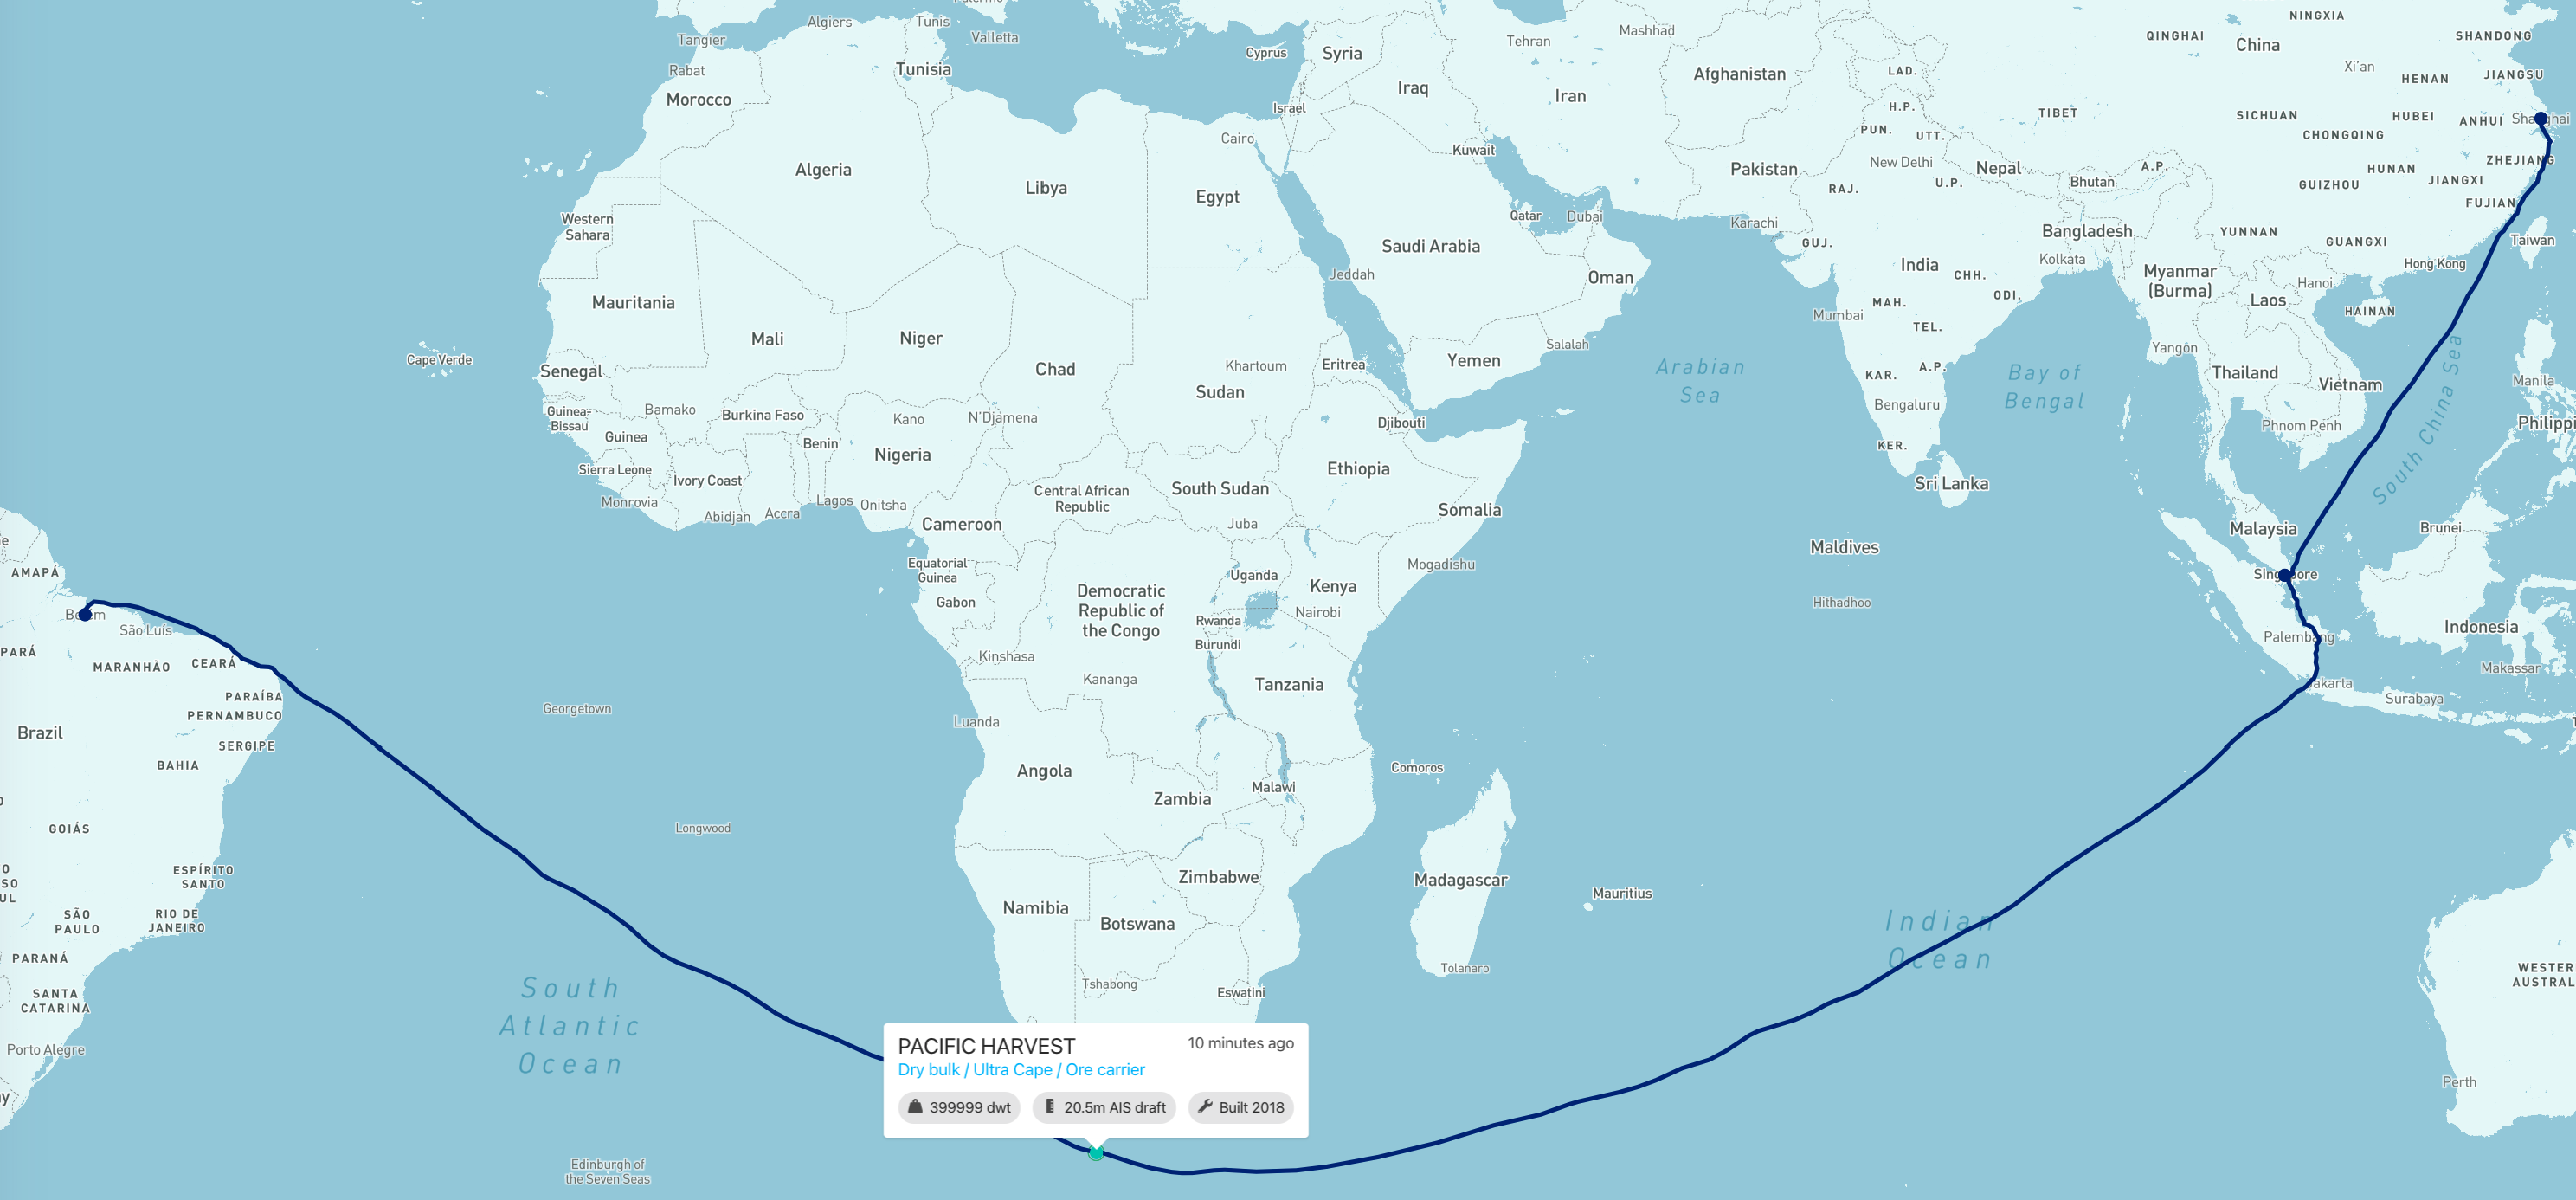
\includegraphics[width=0.9\textwidth]{figures/mo_voyage}
    \caption{Example voyage, created using \acrshort{mo}'s route planner tool, for a traveling vessel (Pacific Harvest), traveling from Brazil to China while stopping at Singapore to refuel.}
    \label{fig:example_voyage}
\end{figure}

To summarize, consider a voyage starting at Brazil and ending in Shanghai, China. Depending on the speed and fuel consumption of the traveling vessel, this voyage is around 12 000 nautical miles long and would take between 30 and 40 days. Thus, it is probable that a traveling vessel would stop to refuel at the bunkering port in Singapore. In this example (shown in \cref{fig:example_voyage}), one could either consider one complete voyage from Brazil to China, or one could consider two voyages; one going from Brazil to Singapore, and another going from Singapore to China. Assuming the vessel use the navigational status ``moored'' in Brazil and China only, the approach used in this thesis would consider one complete voyage from Brazil to Singapore, while a clustering-based method would consider the two shorter voyages.

\subsection{Trajectory similarity}

As will be further elaborated on in \cref{chap:related_work}, the current literature related to vessel destination predictions almost exclusively rely on some form of trajectory similarity. Therefore, trajectory similarity is also included in this thesis' proposed approach to vessel destination prediction. There are three main categories of trajectory similarity measurements: spatial, temporal, and tempo-spatial. Regarding vessel trajectories derived from \acrshort{ais}, they are not likely to share similar time intervals values as vessels travel at different speeds and at different times, therefore, for the purpose of this thesis, only spatial trajectory similarity measures are considered. This assumption is further corroborated by \cite{Zhang2020AISApproach} that arrived at a similar conclusion in their work developing a \acrfull{ml} -based approach to trajectory similarity measurements.

There are a number of spatial trajectory comparison methods that have been widely used for different purposes. The most relevant are the Hausdorff distance \parencite{magdy2015}, Fréchet distance \parencite{magdy2015}, and \acrfull{sspd} \parencite{besse2015review}. Out of these, the \acrshort{sspd} method is the most appropriate as it handles trajectories of different shapes and lengths well which is beneficial when comparing a trajectory from an ongoing vessel voyage to a set of complete historical ones. \cref{fig:sspd} shows an example from \cite{besse2015review} where two trajectories are compared and their symmetric distances are calculated.

\begin{figure}[htbp]  % order of priority: h here, t top, b bottom, p page
    \centering
    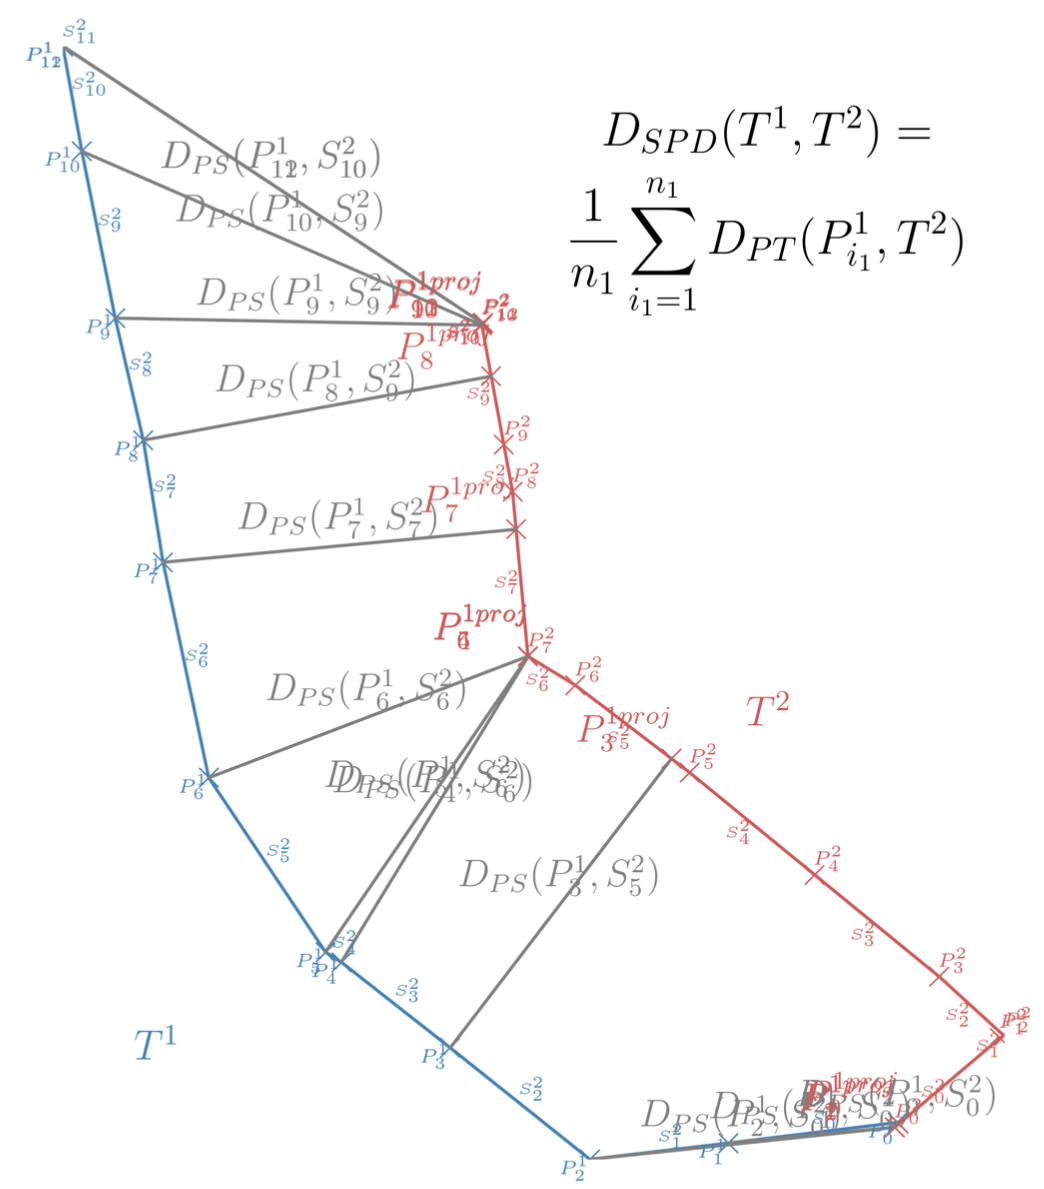
\includegraphics[width=0.5\textwidth]{figures/sspd}
    \caption{Segment Path Distance (SPD) in the SSPD process of comparing two different trajectories \parencite{besse2015review}}
    \label{fig:sspd}
\end{figure}

The methods mentioned thus far are all algorithmic approaches to measuring similarities between trajectories, however, there are also \acrshort{ml}-based methods as well such as the approach proposed in \cite{Zhang2020AISApproach} that also compares their results to the aforementioned methods. They used a \acrfull{rf} to measure similarities between a traveling trajectory and every historical trajectory traveling from the same departure port in order to predict the next destination port for a vessel. They achieved a higher general accuracy when compared to algorithmic methods such as \acrshort{sspd}. Moreover, for similar purposes, some unsupervised clustering methods have also been applied to similar problems such as the \acrfull{dbscan} which is capable of sequentially finding patterns in points and trajectories. This approach is more frequently used in trajectory predictions on a small geographical extent such as for collision detection and anomaly detection.

\subsection{Machine learning (ML)}

\begin{figure}[htbp]  % order of priority: h here, t top, b bottom, p page
    \centering
    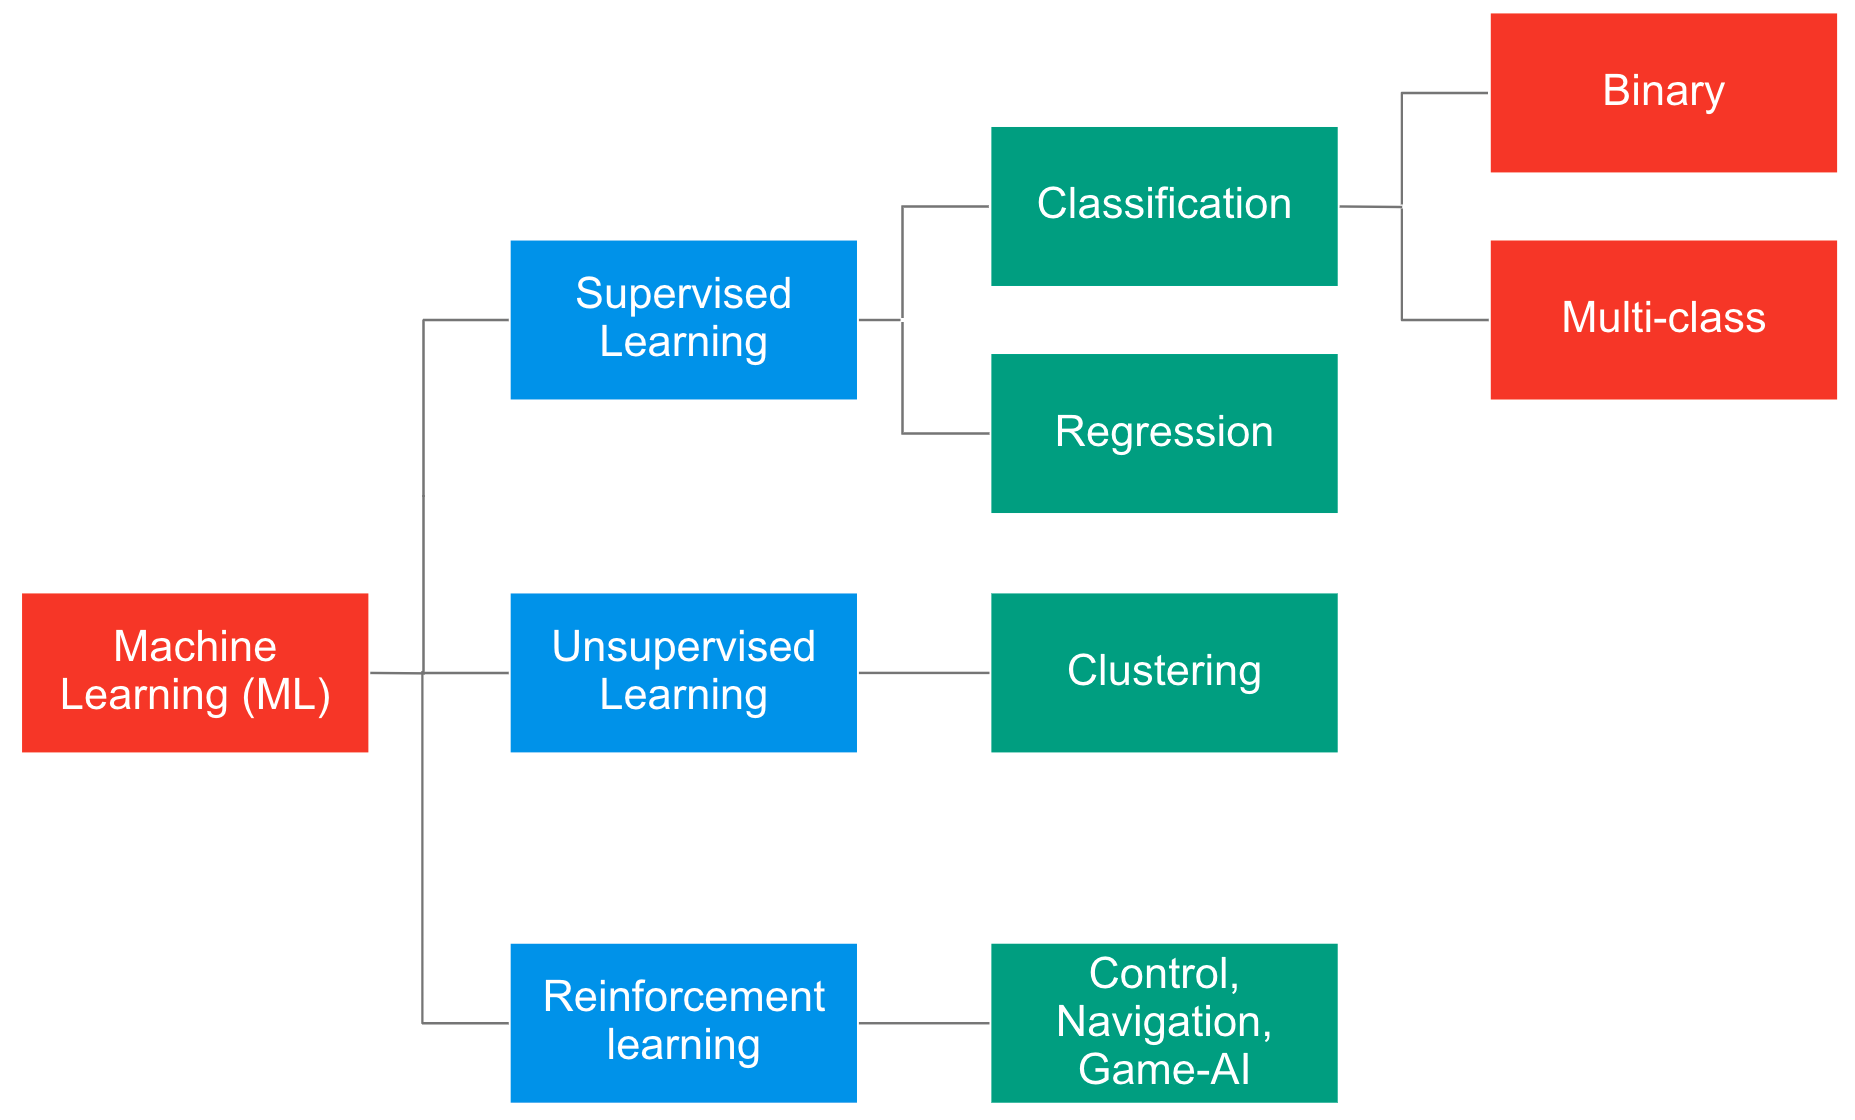
\includegraphics[width=0.75\textwidth]{figures/ml-terms}
    \caption{Machine Learning (ML) hierarchical terminology}
    \label{fig:ml_terms}
\end{figure}

\acrfull{ml} is an umbrella term describing computer algorithms that automatically adapt and improve based on experience. There is a vast number of different \acrshort{ml} algorithms applied to different problem areas. \acrshort{ml} is mainly divided into three broad categories: supervised learning, unsupervised learning, and reinforcement learning. In supervised learning, in the training process, both input and the desired output are provided to the model. The model finds patterns and correlations between input and output data during the training process, and when the model is trained or fitted, it is capable of guessing output given only input. In unsupervised learning, no output labels are provided to the model leaving the model to find patterns in the input set on its own. Clustering is an example of unsupervised learning as the model finds and labels patterns in input data without any external guidance. Reinforcement learning is a dynamic approach to \acrshort{ml} where the model continuously learns while trying to achieve a goal. In this method, the model navigates a problem space, and the program rewards or punishes the model that tries to optimize for rewards. In regards to topics covered by this thesis, \acrshort{ml}-based trajectory comparisons involve unsupervised learning, while predicting destination ports is supervised as the historical destinations are known.

\begin{figure}[htbp]  % order of priority: h here, t top, b bottom, p page
    \centering
    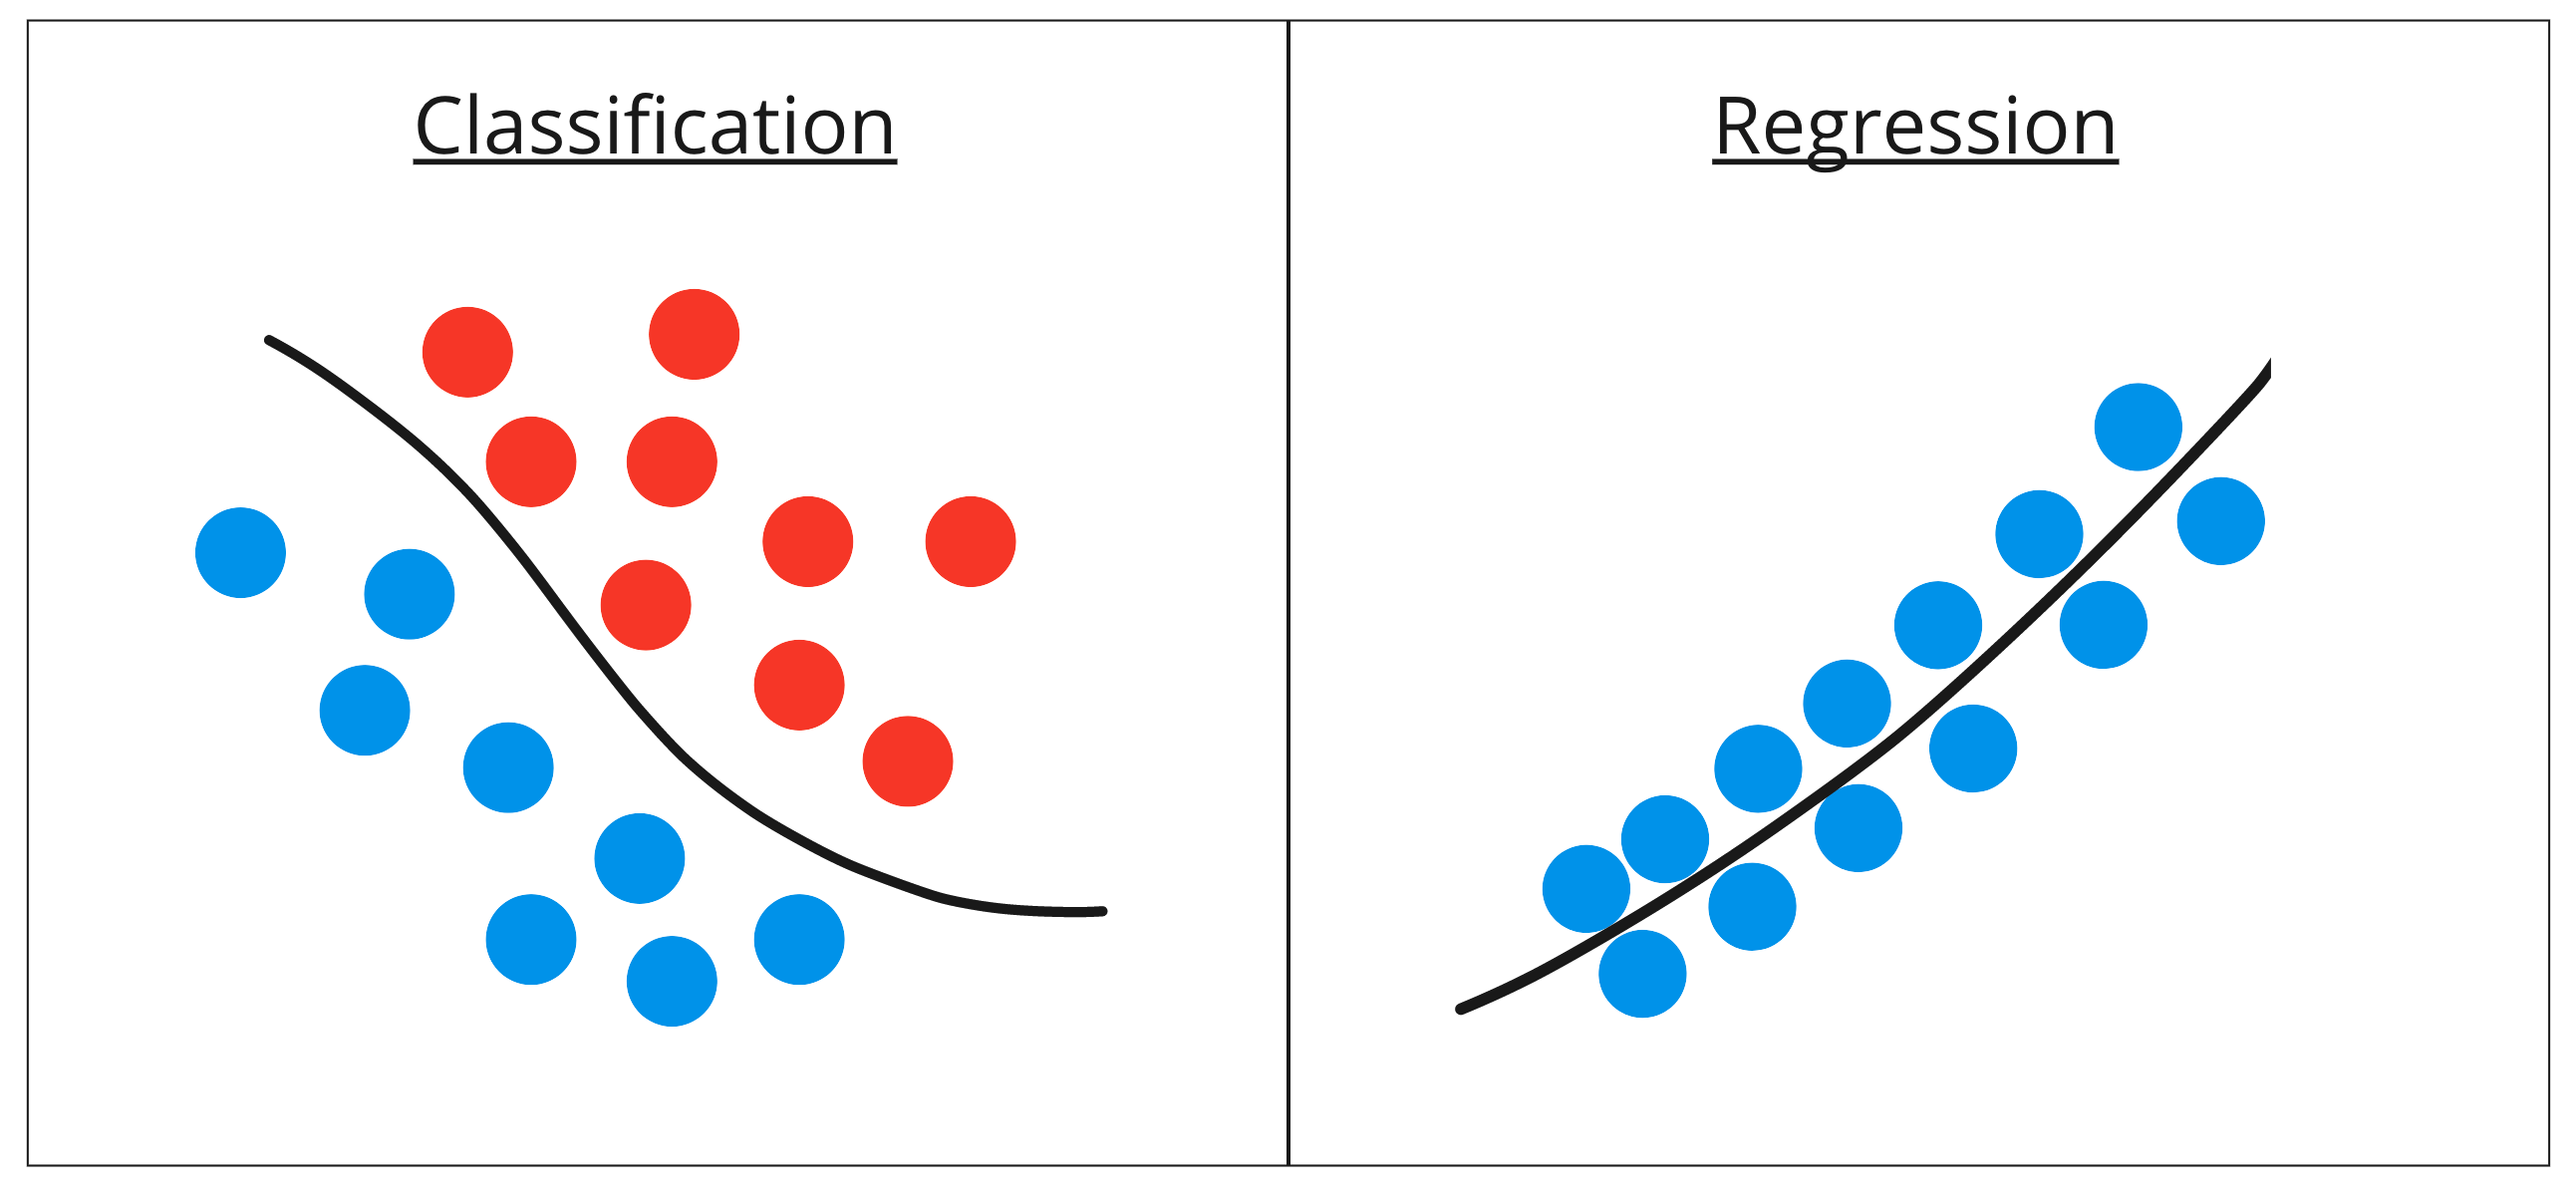
\includegraphics[width=0.75\textwidth]{figures/class_regg}
    \caption{Example showing the difference between classification and regression tasks}
    \label{fig:classification_regression}
\end{figure}

Moreover, supervised learning can further be divided into regression and classification problems. The main difference between the two is that classification aims at predicting a label, or a class, while regression predicts a quantity that is not necessarily present in the training data. For instance, a regression model can be used to predict the price of an item for sale, while classification can be used to label emails as "spam" or "not spam". \cref{fig:classification_regression} shows the difference between classification and regression. The example of classifying emails as ``spam'' or ``not spam'' would be considered a binary classification problem as there are only two possible labels, however, classification can also involve predicting more than two outcomes which is commonly referred to as multi-class classification. In the context of this thesis, predicting a vessel's destination port can be formulated as a multi-class classification problem as every possible destination port are different possible labels for a given voyage in progress. \cref{fig:ml_terms} shows the how \acrshort{ml} is hierarchically divided into more specific terms relevant for the scope of this thesis.

\begin{itemize}
    \item Cross-validation
    \item Hyperparameter optimization
\end{itemize}

\section{Technologies and protocols}

\subsection{Database system}

All the data that is used throughout this thesis for analysis is collected and stored in a \textit{PostGreSQL} database. \textit{PostGreSQL}, or \textit{Postgres}, is an open-source object-relational database management system that supports the extended subset of SQL standards. One major advantage of using \textit{Postgres} is the support for plugins such as \textit{PostGIS} that provides tools for dealing with \acrshort{gis} and geometric data. In this thesis, \textit{PostGIS} is frequently used to store and process geographical trajectory data for vessel voyages. Throughout this thesis, when referring to the proposed methodology and results, terms such as database, table, row, and column refers to the \textit{PostGreSQL} database used and its tables with rows, and columns.

\subsection{Programming languages and tools}

The main programming languages used throughout this thesis are Golang and Python. Golang is primarily used in constructing the initial data foundation which requires dealing with databases, trajectory building and validation. Golang is chosen for this because of its performance benefits and ease of use. For data analysis and machine learning, Python is the main programming language of choice. Most code provided to the reader in this document is written with the focus of readabilty over efficiency.

\subsection{Automatic Identification Systems (AIS) data}
\label{sec:ais_data}

\begin{figure}[htbp]  % order of priority: h here, t top, b bottom, p page
    \centering
    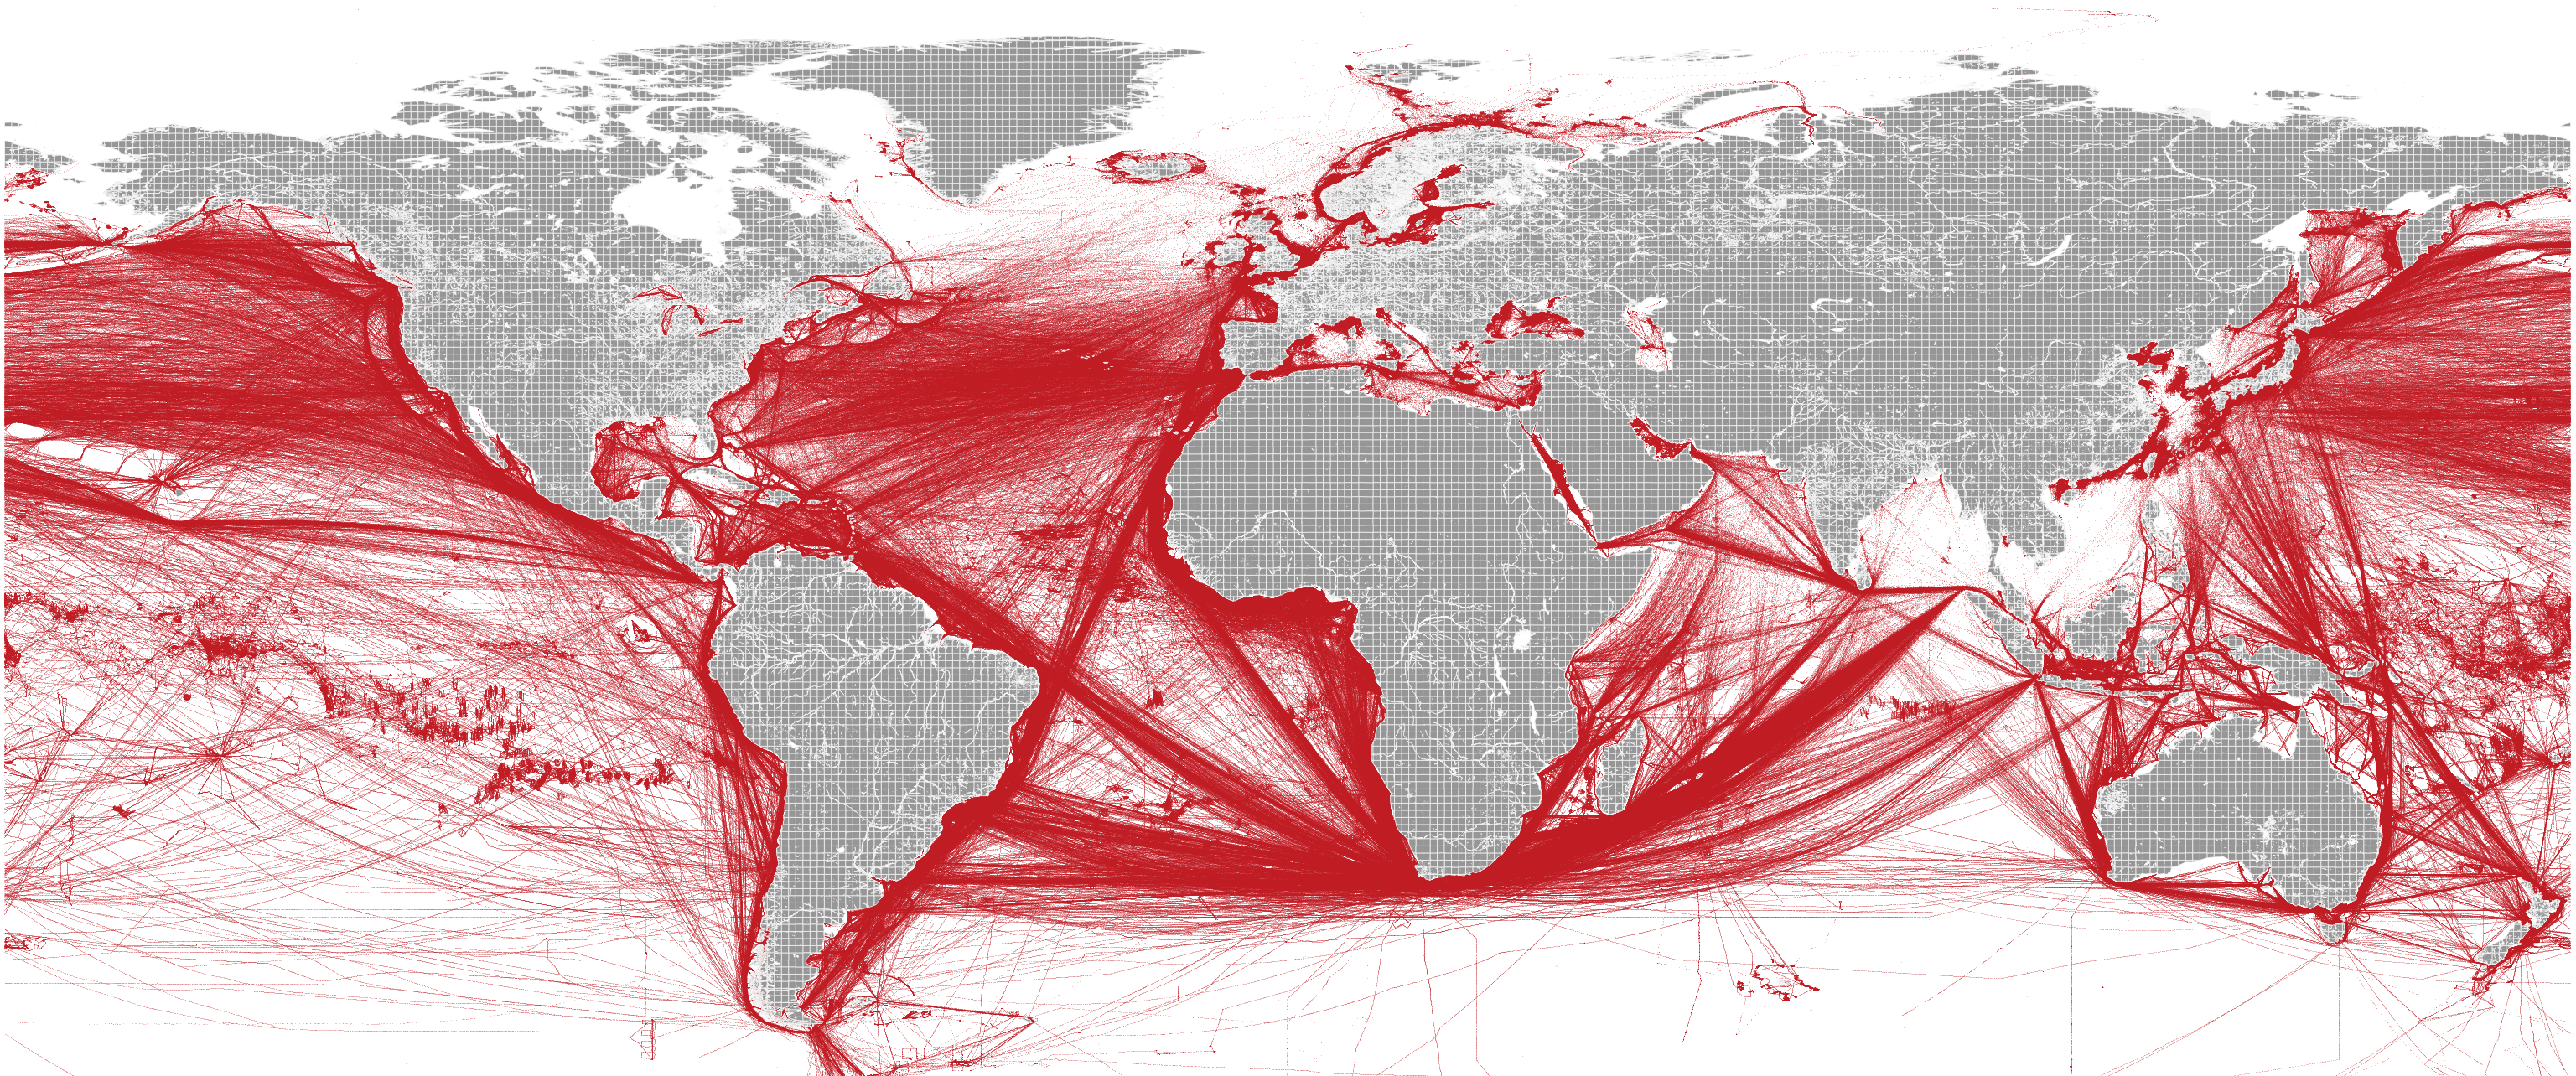
\includegraphics[width=1.0\textwidth]{figures/ais_history}
    \caption{Vessel positions derived from 100 million AIS positional reports}
    \label{fig:ais_positions}
\end{figure}

As already mentioned in \cref{sec:topics_covered}, \acrfull{ais} was initiated by \acrfull{imo} and since 2004 every commercial and passenger vessel exceeding 299 \acrfull{gt} is required to carry an \acrshort{ais} transmitter. These transmitters broadcasts \acrshort{ais} messages following the \gls{aivdm} protocol. The \gls{aivdm} protocol contains two main types of reports: positional and static. The positional reports contains automatically collected information such as the transmitting vessel's \acrfull{mmsi} number, the current timestamp, and the vessel's current navigational data including the current geographical coordinates, \acrfull{sog}, \acrfull{cog}, true heading, \acrfull{rot}, and more. The static reports contain additional information about the vessel and its current voyage, some of which are manually inputted, such as the vessel's \acrshort{imo} number, name, dimensions, draft, intended destination and \acrfull{eta}. As an example, \cref{fig:ais_positions} shows a visualization of 100 million \acrshort{ais} randomly chosen positional reports from a collection of historical \acrshort{ais} positions for global collection of shipping vessels. In relation, the historical \acrshort{ais} dataset used in this thesis consists of more than one billion records ranging from December 2019 to February 2021.

Regarding vessel identification in the \gls{aivdm} protocol, there are mainly two values that are unique to a given vessel: the \acrshort{mmsi} and \acrshort{imo} numbers. Either of these should be unique on their own for a given vessel, however, \acrshort{mmsi} numbers can be recycled under certain conditions such as when a vessel is put out of commission while the \acrshort{imo} number is specific to a vessel's hull. Therefore, \acrshort{imo} is the preferred identifier, however, since the \gls{aivdm} protocol divides these identifiers into positional and static reports, both need to be considered in order to use both static and positional \acrshort{ais} information.

\section{Initial data foundation}

This section describes the form and meaning of the data that forms the foundation of the thesis' proposed solution. The data is provided by the collaborative company \acrfull{mo} to the author.

\subsection{Vessel departure and arrival detection}
\label{sec:vessel_transitions}

\acrshort{mo} collects live \acrshort{ais} messages provided by a few sources, and in addition, they keep track of their navigational statuses as they are transmitted in the \gls{aivdm} protocol. These status attributes describe the current navigational state of the vessel for purposes of planning and security. Implicitly, these messages can indicate that a vessel has arrived or departed from a given port which can be used to detect voyages. When a vessel has concluded her journey and arrives at a port, the navigational status is changed to \textit{"MOORED"}, and when departing a port, the status is changed to \textit{"UNDERWAY USING ENGINE"} or \textit{"UNDERWAY SAILING"}. There are also other navigational statuses that could be relevant for voyage information such as \textit{"AT ANCHOR"} which could indicate that a vessel is bunkering (refueling) or is waiting for access to a berth that is congested. Currently, transitions from a status that indicates that a vessel is moving to the status \textit{"MOORED"}, and from \textit{"MOORED"} to moving are collected and labeled as arrivals and departures from or to the closest port within a given radius. This has proven to be a good method of identifying voyages and voyage trajectories between two ports as positions transmitted between a departure and arrival can be collected into a voyage trajectory that can be compared to other trajectories for analytical purposes. Throughout this thesis, this concept is referred to as vessel transitions.

\subsection{Additional vessel information and segmentation}
\label{sec:vessel_info_segments}

\acrshort{mo} has implemented a system for categorizing vessels into different segments, subsegments, and further variations. These segmentations are based on various factors such as the dimensional data provided by \acrshort{ais} messages as well as details provided by external vessel information sources and even user and manual input. The most important factors are the vessel type from the \gls{aivdm} protocol and the carry range, measured in \acrshort{dwt}, of the vessels which indicates how much cargo it can carry. This segmentation of vessels is highly relevant to voyage patterns as vessels of different types and sizes travel to different ports and countries for different shipping companies. This is further shown in \cref{fig:segment_map} which shows, from an image of \acrshort{mo}'s web platform, how different subsegments of the dry bulk cargo segment travels in different areas of the world. Since this categorization provides valuable insights into voyage patterns, vessel segmentation values are included in this thesis' proposed approach to vessel destination prediction.

\begin{figure}[htbp]  % order of priority: h here, t top, b bottom, p page
    \centering
    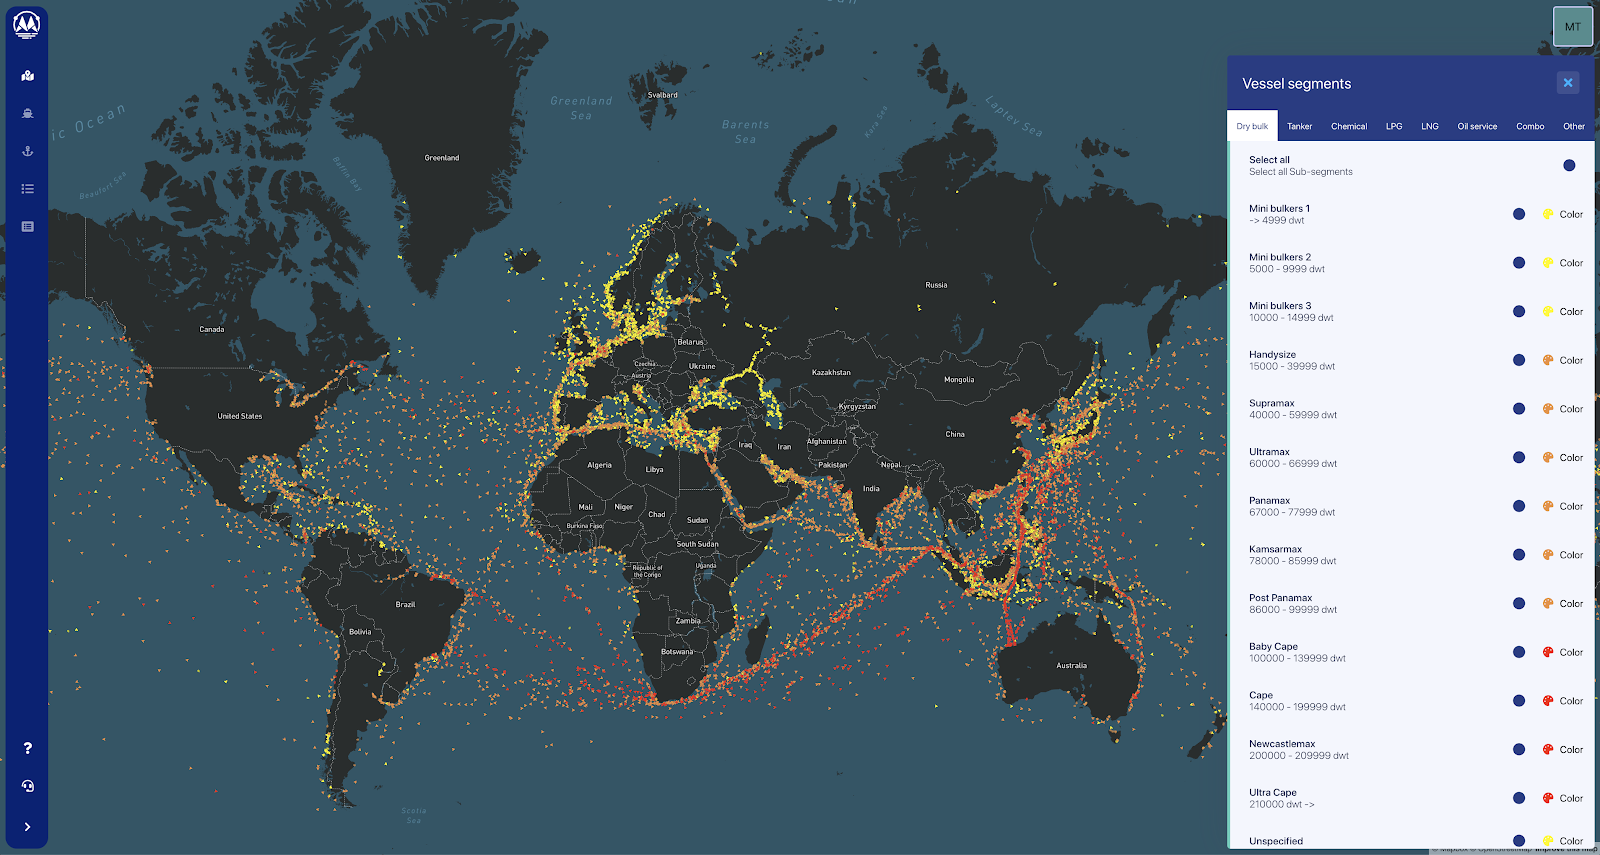
\includegraphics[width=1.0\textwidth]{figures/segment_map}
    \caption{\acrfull{mo}’s segmentation of vessels where yellow vessels are smaller than reds}
    \label{fig:segment_map}
\end{figure}

Moreover, \acrshort{mo} also has extensive vessel details for every vessel structured as a questionnaire in their product. This vast questionnaire contains information and fields from a combination of standards in the industry such as Q88\footnote{\url{https://corp.q88.com/}}. Data for the questionnaire is also collected from a number of external sources such as IHS Merkit\footnote{\url{https://ihsmarkit.com/index.html}} and DNV\footnote{\url{https://www.dnv.com/}}. Users of \acrshort{mo} also have the possibility of suggesting changes to a public version of this questionnaire for any vessel. These changes are verified by \acrshort{mo} and published if the information proves accurate. This detailed description of vessels provides creates a big potential for data analysis and a potential \acrshort{ml} model that is highly aware of specific vessels which ultimately may affect its traveling patterns. However, in this thesis, the main focus is on the vessel segmentation when developing the proposed solution. This data is later referred to as vessel segments and includes both the vessels' segment and sub-segment.

\subsection{Shipping ports}
\label{sec:shipping_ports}

\acrshort{mo} has an extensive port database containing more than 5600 ports. From sources such as UNECE it is possible to find a vast number of ports, however, only a sub-set of the worlds known ports are used by \acrshort{mo} as these are considered relevant shipping ports. The process of determining what ports are relevant shipping ports is a continuous manual process in \acrshort{mo} but it ensures that the available selection of ports is highly relevant for the industry. Furthermore, all ports are identified by their \gls{locode}. This is a five-letter unique identifier provided and managed by the United Nations (UN). In the five-letter code, the first two indicate the port's country of origin, while the three last indicate a more specific location within the origin country. As an example, the \gls{locode} for the port of Oslo is \texttt{NOOSL} where ``NO'' stands for Norway, and ``OSL'' stands for Oslo. For comparison, a similar system is used for international airports. For this thesis, only the 5600 relevant ports are considered for the analysis.

\chapter{Related work}

The topic of \acrfull{ais} -based predictions has already been explored quite extensively, especially in recent years as \acrshort{ais} systems has become an enforced standard for commercial vessels in the industry. However, the \acrshort{ais} standard has mainly been standardized for the purpose of maritime safety and navigation, and the existing academic work on this topic reflects this. Therefore, most of the related work consists of vessel trajectory predictions for the purpose of foreseeing a future collision situation or for detecting anomalies from detected shipping lanes. These types of predictions are applicable for predicting a vessel's future position in a short time interval, in a smaller geographical scale, but with high positional accuracy.

In order to establish the current state of the art of the topic area and establish to what extent the literature answers the proposed research questions, a literature review was conducted which is explained in this section.

\section{Literature review}
\label{sec:lit_review}

As already mentioned, based on initial research into the thesis' topic area, there seemed to be an apparent trend in motivations of related work directed at short-term predictions for safety and navigational purposes. In contrast, this thesis aims at using \acrshort{ais}, and other attributes, for longer term predictions, or more accurately, port destination predictions. However, because of the exploratory nature of thesis, the literature review conducted was broad in order to include work that might have taken a different approach to solve the same problem. In order to organize the resulting papers, a categorical separation of papers based on motivation was defined as follows:

\begin{enumerate}
\setcounter{enumi}{-1}
    \item The paper's motivation deems it completely irrelevant to the topic area.
    \item The paper's motivation includes vessel predictions, but on a smaller time or geographical scale making it irrelevant for comparison.
    \item The paper's motivation includes destination predictions making it relevant enough for further analysis.
\end{enumerate}

\textit{Category 0} is defined to filter out papers that were irrelevant but could not be excluded by narrowing the search query. \textit{Category 1} includes paper that relates to the established trend mentioned earlier where the proposed method seems relevant on a small scale, but is ultimately not applicable to the thesis' problem area. It also includes papers that considers relevant topics but not relevant solutions. Finally, the papers labeled with relevancy \texttt{2} falls within \textit{Category 2} and includes papers that falls within the same topic area and are relevant for further analysis in regards to the research questions.

In order to determine what papers fitted \textit{category 1} and \textit{2}, papers with a relevance higher than zero were further analyzed in order to determine the following attributes:

\begin{itemize}
    \item Motivation and goals
    \item Data source
    \item Prediction method
    \item Geographical extent
    \item Time interval
    \item Validation method
    \item Validation, or performance metrics
\end{itemize}

In this literature review, the primary search engine used was \textit{Scopus}\footnote{\url{https://www.scopus.com/}} as it seemed to return the best search results without an excess of less relevant papers that was returned by other search engines such as \textit{ScienceDirect}\footnote{\url{https://sciencedirect.com}} and \textit{Google Scholar}\footnote{\url{https://scholar.google.com}}. Furthermore, the chosen search query was also ran on the \acrshort{ntnu} university library \textit{Oria}\footnote{\url{http://ntnu.oria.no/}} in order to find overlap and additional results not found by \textit{Scopus}.

\subsubsection{Search query and filters}

The objective of the literature review was to conduct a broad search detecting papers related to multiple relevant topics such as \textit{vessel destination prediction}, \textit{vessel trajectory prediction}, \textit{vessel availability forecasting}, and \textit{maritime logistics}. Therefore, the search query used in the literature review was designed to find papers within multiple topics and was derived at from testing multiple queries on multiple search engines.

For instance, the following queries were tested using the search engine provided by \textit{ScienceDirect}:

\begin{itemize}
    \item `vessel trajectory' OR `ship trajectory' resulted in \textbf{421} papers
    \item ais AND (`vessel trajectory' OR `ship trajectory') resulted in \textbf{150} papers
    \item ais AND (prediction OR predicting) AND (`vessel trajectory' OR `ship trajectory') resulted in \textbf{108} papers
\end{itemize}

The above queries returned a large number of papers relevant to \textit{category 1}, so in order to find more relevant papers, more specific queries were also tested:

\begin{itemize}
    \item `vessel destination' OR `ship destination' OR `vessel availability' resulted in \textbf{389} papers
    \item ais AND (`vessel destination' OR `vessel availability') resulted in \textbf{25} papers.
    \item ais AND (predicting OR forecasting) AND (`vessel destination' OR `vessel availability' OR `ship supply') resulted in \textbf{18} papers.
\end{itemize}

The search terms that seemed to return the most relevant papers was combined into the final query used in the literature review shown in \cref{lst:search_query}.

\begin{lstlisting}[
    caption={Search query used in literature review},
    label=lst:search_query
]
ais AND (
    predict OR predicting OR forecast OR forecasting
) AND (
    vessel OR ship OR maritime
) AND (
    destination OR availability OR supply OR trajectory OR logistics
)
\end{lstlisting}

Moreover, the following filters was used to limit the search result:

\begin{itemize}
    \item The paper must be published in the last 5 years.
    \item The paper must be available in English.
    \item The paper must be available using the access rights provided by \acrshort{ntnu}.
\end{itemize}

As already mentioned, the search query was ran on the search engine \textit{Scopus}, thus the search query and filters was modified to the search engine's format as shown in \cref{lst:search_query_scopus}.

\begin{lstlisting}[
    caption={Search query used in Scopus including filters},
    label=lst:search_query_scopus
]
TITLE-ABS-KEY (
    ais AND (
        prediction OR predicting OR forecast OR forecasting
    ) AND (
        vessel OR ship OR maritime
    ) AND (
        destination OR availability OR supply OR trajectory OR logistics
    )
) AND PUBYEAR > 2014 AND (
    LIMIT-TO ( DOCTYPE , "cp" ) OR
    LIMIT-TO ( DOCTYPE , "ar" ) OR
    LIMIT-TO ( DOCTYPE , "re" ) OR
    LIMIT-TO ( DOCTYPE , "ch" ) OR
    LIMIT-TO ( DOCTYPE , "Undefined" )
) AND ( EXCLUDE ( SUBJAREA , "MEDI" ) )
\end{lstlisting}

\subsubsection{Results}

The defined search query returned a total of \textbf{80} papers from the \textit{Scopus} search library and \textbf{22} from \textit{Oria} where out of which \textbf{7} papers did not overlap with results from \textit{Scopus}. These \textbf{87} papers formed the basis of the literature review.

The papers were evaluated based on the level of relevance as defined in \cref{sec:lit_review}. Out of the \textbf{80} papers, \textbf{49} fell within \textit{category 0}, \textbf{32} within \textit{category 1}, and \textbf{6} within \textit{category 2}.

The large number of irrelevant papers resulted from the broadness of the query that was designed to find results in multiple topic areas. Furthermore, there were some papers that was medical in nature but not labeled correctly in \textit{Scopus} and was returned as the term \acrshort{ais} is also an acronym of \textit{Arterial Ischemic Stroke}. Some papers were also not publicly available but was not excluded by the search, while other papers were deemed irrelevant as they concerned topics such as mapping fishing areas in a specific region, power and performance predictions using \acrshort{ais} data, or high level discussions of potential applications of \acrshort{ais} data analysis.

The large number of papers within \textit{category 1} further confirms the general trend of \acrshort{ais} -based predictions as the primary goal of most of the resulting papers were to predict future positions of vessels within a shorter time intervals for the purpose of either safety and navigation or anomaly detection. None of the papers within \textit{category 1} seemed applicable to predict vessel destination ports at a global scale, however, for reproducibility, all papers with a relevancy of \textit{1} are listed in \todo{APPENDIX}.

% most relevant papers collected from literature review
\begin{table}[tbp]
    \centering
    \csvreader[
      tabular=p{0.55in} p{1.7in} p{1.6in} p{0.7in} p{0.3in},
      table head=\hline \bfseries{Paper} & \bfseries{Goal} & \bfseries{Pred. method} & \bfseries{Geo-extent} & \bfseries{Time},
      before line=\\\hline,
      late after last line=\\\hline % horizontal line at the end of the table
    ]{
        csvtables/most_relevant.csv
    }{}{\csvlinetotablerow}
\caption{Papers collected from literature review with relevant geographical and time limitations}\label{tab:most_relevant_papers}
\end{table}

The remaining \textbf{}6 papers (listed in \cref{tab:most_relevant_papers}) were deemed relevant enough to further analyze in order to answer the research questions defined in \cref{sec:research_questions}. In addition, \cite{lechtenberg2019}, which was discovered during the process of testing queries, was also included in the analysis as it seemed highly relevant toward availability forecasting, but did not appear when using the two search engines in the final review.


\todo{copied from RPP}
\paragraphheader{RQ 1: What prediction methods can be used to predict vessel availability?}

\cite{lechtenberg2019} used a combination of several prediction methods in order to predict vessels’ next destination region, estimated time of arrival (ETA), and anchor time (AT) within regions. For predicting the next destination region the \textit{Markov Decision Process} was used as there are a limited number of possible regions (44) that a vessel can travel to. For the ETA and AT predictions, an \textit{XGBoost} method was applied. However, the extent of the regions was not disclosed, and although it was explained that port frequencies were used to determine regional availability, the accuracy of port frequencies was also not disclosed.

\paragraphheader{RQ 2: What prediction methods can be used to predict vessel destinations?}

\cite{ZHANG2020102729} was the second paper found which fitted within \textit{category 1}, and used a random forest approach to compare a given vessel’s current trajectory with all historical trajectories from the same departure port. They also used port frequency to normalize the results. In this way, they managed to achieve good results by combining both methods for predicting port destinations as well as city destinations. This method was unique as it considers multiple aspects of vessel voyages compared to the other methods.\\

\paragraphheader{RQ 2A: What type of data did they rely on?}

All of the aforementioned methods relied on historical AIS data collected by a combination of satellite and land-based base stations. \cite{ZHANG2020102729} also relied on an extensive port data base consisting of over \textbf{10 000} ports.

\paragraphheader{RQ 2B: How much depth of the data was relevant to the results?}

\cite{ZHANG2020102729} exclusively relied on the navigational data supplied by the AIS protocol. The navigational part of the AIS protocol includes coordinates, speed over ground (SOG), rate of turn (ROT), course over ground (COG), and more. Furthermore, \cite{ZHANG2020102729} also considered port frequencies, however, this frequency is deducted from the navigational part of the AIS data. Similarly, \cite{lechtenberg2019} also used port frequencies to predict regional availability, ETA, and AT. As already mentioned in \cref{sec:problem_desc}, destination and ETA values are included in the AIS protocol, however, as they are manually inputted by crew members they are not accurate. This is reflected in the existing literature as none of the aforementioned methods takes these values into consideration. Thus, it seems that all the relevant research ultimately only considers the navigational part of the AIS protocol for future predictions.

\paragraphheader{RQ 2C: How successful were they at predicting vessel destinations?}

\cite{lechtenberg2019} claims a \textit{98\%} accuracy when it comes to predicting a vessel’s next region, however, this value is presumed to vary depending on the size of the regions which is not disclosed in the paper. \cite{ZHANG2020102729} claims to have achieved a \textit{66.57\%} accuracy level for port-based predictions and \textit{81.65\%} accuracy for city-based predictions. As there is very little research that directly concerns predicting port or region destinations it is hard to establish a general accuracy of the state of the art. The closest assumption would be around \textit{70\%} for port predictions and \textit{98\%} for region predictions.

\paragraphheader{RQ 2D: How applicable were they toward predicting vessel availability?}

\cite{lechtenberg2019} was directly applicable and applied toward predicting vessel availability with a global set of regions. \cite{ZHANG2020102729} was not directly applied to forecast availability although it shows a very promising and generic method of predicting vessel’s future destinations unrestricted from time intervals or geographical areas. It is therefore very applicable toward predicting availability if applied to a global set of vessels. The rest of the aforementioned papers does not seem applicable toward availability if not combined with other methods that enable them to give accurate predictions globally.

\paragraphheader{RQ 3: How can the quality of the prediction methods be ensured?}

\cite{lechtenberg2019} does not go very in-depth on this topic, however, the paper mentions dividing the data into \textit{90\%} training data and \textit{10\%} test data. The accuracy metric is taken from how much of the test data was accurate. \cite{ZHANG2020102729} did an extensive evaluation of their method including the five-folder cross-validation method to ensure the model is not over-fitted. This process includes dividing the data into five “folders” and using one folder at a time for evaluation and the others for training. If the general accuracy does not vary much across the evaluation folders, the model is not overfitted.

\paragraphheader{RQ 3A: What metrics, or measurements, are used to establish quality?}

It seems that accuracy is the main measurement used to establish quality. Furthermore, \cite{lechtenberg2019} mentions using both the “mean absolute error” (MAE) and the “root mean square error” (RMSE) as quality indicators. \cite{ZHANG2020102729} mainly uses “average prediction distance error” (APDE) as their quality indicator which is based on the distance between the predicted trajectory and the actual trajectory.

\paragraphheader{RQ 4: How extensive is the impact of considering segmentation for prediction methods?}

None of the papers found within the research areas considers any type of segmentation of vessels. It is, therefore, impossible to answer this research question based on the current state of the art of the problem area.


\begin{sidewaystable}
    \centering
    {\small
    \begin{tabular}{|l|l|l|l|l|l|l|}
    \hline
        Paper & Motivation & Prediction method & Geographical scale & Time scale & Validation method & Validation metrics \\ \hline
        \cite{Alizadeh2020PredictionTrajectory} & trajectory similarity measurement for prediction of positions at time intervals & "spatial distance, bi-directional distance, speed distance" & "region (strait of georgia, USA)" & "10, 20, 30 minutes" & "sorenson similarity index (SSI), case study in region" & accuracy \\ \hline
        \cite{Alizadeh2021VesselData} & Vessel trajectory prediction for collision avoidance & "LSTM (RNN) with trajectory distance similarity measurements (TSSP, PSSP, TSSPL)" & "Strait of Georgia, USA" & Short term (10 - 40 mins) & 1 to 8 division of training and validation set & haversine distance accuracy (0.8 km to 3.5 km from 10-40 mins) \\ \hline
        \cite{Borkowski2017TheFusion} & data fusion prediction for collision avoidance integrated in navigation system & "ANN, data fusion, GRNN" & small (collision avoidance) & small & integrated and tested in real naviagtional system & RMSE \\ \hline
        \cite{Brandt2017MovingPrediction} & short time predictions of moving objects & "moving object data stream mangement systems, kNN " & "small, region in US" & small (10 minutes) & test cases & not explained \\ \hline
        \cite{Burger2020DiscretePrediction} & trajectory predictions for filling in gaps in AIS data & "DKF (discrete kalman filters), LRM" & small & small & single cases analysis on a vessel comparing two models & MED (mean euclidea distance) \\ \hline
        \cite{Chen2020ThePrediction} & cluster reconstruction not requiring training phase for short time frames & NPC clustering finding best possible next points & small & small & extensive comparisons with other methods & "accuracy, distance error" \\ \hline
        \cite{Dalsnes2018ThePrediction} & collision detection for autonomous vessels & NCDM & small (collision detection) & small (collision detection) & 90/10 training validation sets & RMSE \\ \hline
        \cite{Dijt2020TrajectoryShips} & collision avoidance for autonomous ships & sequence to sequence neural network & small (collision avoidance) & small (collision avoidance) & "90/10 data split of six hours trajectories, cross folder validation" & "absolute trajectory error, RMSE, MAE" \\ \hline
        \cite{DIng2020ALSTM} & longer time and multidimensional trajectory predictions & LSTM & small & 5-20 minutes & "training, validation, test set (8:1:1)" & MSE \\ \hline
        \cite{Forti2020PredictionNetworks} & sequence-to-sequence RNN approach & RNN with LSTM encoder-decoder architecture & region & small & 5-fold cross validation & RMSE \\ \hline
        \cite{Guo2018TrajectoryChain} & trajectory predictions MDTN (mobile delay tolerant network) & k-order multivariate markov chain & region (grid based) & small & "simulation, experiments" & accuracy \\ \hline
        \cite{Hexeberg2017AIS-basedPrediction} & collision detection & single neighbor search (SPNS) & region (trondheim) & small (10 minutes) & "training, validation sets, manually selected scenarios, validate with real trajectory" & RMSE \\ \hline
        \cite{Jin2020MaritimeNetwork} & longer range predictions for security motivations & "RNN, LSTM" & regional/small & small & model simulation & "distance accuracy over time, MAE, SSE" \\ \hline
        \cite{Kim2018PreprocessingArea} & predictions for Vessel Traffic Service (VTS) & NN & small & small & case study on region & speed and distance error \\ \hline
        \cite{Li2018ShipMining} & ceaner data extraction and mining for predictions & RBF neural network model & small (tested on river in china) & small-medium (hours) & simulation/case study on river in china & trajectory difference from real to simulated \\ \hline
        \cite{Li2019Long-termData} & longer term predictions for collision avoidance & "LSTM, longest comomon subsequence(LCS) algorithm, DBSCAN clustering" & small / collision avoidance & small / collision avoidance (15 min) & "applied to 4 regions, case studies" & distance error \\ \hline
        \cite{Lian2019ResearchAlgorithm} & "investigating particle filtering, near prediction, least squares estimation approach to predictions for smaller scale predictions" & "linear prediction, least squares, particle filtering" & small / collision avoidance & small / collision avoidance & "simulation, 9 hours of data" & "distance error, speed error" \\ \hline
        \cite{Liu2019VesselACDE-SVR} & trajectory prediction that also handles real time at sea & "SVR, ACDE, RNN" & small / collision avoidance & small / collision avoidance & training/validation sets & distance error \\ \hline
        \cite{Liu2020PredictingLearning} & "predicting trajectories for ship management, interpolating method for filling in missing AIS in trajectory" & "LSS-VM (least-squares support-vector machines) for predictions, cubic spline function to regulate trajectories via interpolation" & "independent of regions, but on a small scale (predicting distance not arrival ports)" & small (predicting next positions in trajectory) & four random trajectories selected for predictions & accuracy in distance/meters from actual trajectory \\ \hline
        \cite{Mao2018AnMining} & database for trajectory prediciton and mining & "interpolating trajectory reconstruction, are of interest bsed grid search, ELM and SLFN for predictions" & region based & medium (20 - 40 minutes) & original vs predicted trajectory & distance error \\ \hline
        \cite{Murray2018AOperations} & collision detection for autonomous vessels & Single point neighboir search method & small (collision detection) & 5-30 minutes & 90/10 training validation sets & RMSE \\ \hline
        \cite{Murray2019AnVessels} & collision avoidance & "gaussian mixture modelling, principle component analysis" & small / collision avoidance & small / collision avoidance & running 100 times randomly selecting points & distance error \\ \hline
        \cite{Murray2020AData} & trajectory predictions for early warnings and safety & "GMM clustering (gaussian mixture model), novel dual autoencoder" & region (tromsø) & 30 minutes (1 year or historical AIS) & distributed accuracy over time in the future (predicted positions vs actual positions) & accuracy at time intervals \\ \hline
        \cite{Rong2019ShipModel} & modelling uncertainty of trajectory predictions & "Bayesion model, Gaussian Process" & small / collision avoidance & "small / collision avoidance (10, 20, 30)" & "case study in region, training / validation data" & "accuracy, distance error" \\ \hline
        \cite{Suo2020ANetwork} & trajectory predictions for early warnings and safety & "GRU (gate recurrent unit), DBSCAN, comp. with LSTM" & tested on single port in china & "small, minutes to hour" & "training, validation, test set (not defined how much)" & accuracy \\ \hline
        \cite{Tafa2019AutomaticPrediction} & synthetic route representation and predictions & "DBSCAN, route similarity probability model" & east china sea region & 10-80 minutes & simulation & accuracy \\ \hline
        \cite{Tang2019ANetwork} & collision avoidance for automonous ships & LSTM & region in china & uses 10 min of data to predict 20 next minutes & training/validation sets & "MAE, MSE" \\ \hline
        \cite{Uney2019DataModels} & forecasting trajectories from historical and streaming trajectories & directed grid based bayesion model / gaussian mixture forecast density & tested on region (15x15 grid) & any (tested with 2 months of data) & real life case study in region & not explained \\ \hline
        \cite{Virjonen2018ShipMethod} & predictions in area in finnland that has to be several hours ahead in time & k-nearest neighbours & medium (region of finnland test case) & "medium, several hours" & nested leave-one-out-cross-validation (LOOCV) & distance accuracy \\ \hline
        \cite{Wang2020VesselGRU} & predicting vessel berthing trajectory for safety and collision avoidance & "Bi-GRU (tensorflow, keras)" & single port in china & small (minutes) & "training, validation set (not defined ratio), compared to other models" & MSE \\ \hline
        \cite{Xiao2020BigTechniques} & "for collision avoidance, better quering, more effective predictions" & "knowledge based particle filtering (PF), MLNN" & "smaller, limited to collision avoidance" & 3-10 minutes & testing different scnarios i.e. case studies & "sog, coc, and distance error" \\ \hline
        \cite{You2020ST-Seq2Seq:Prediction} & sequence-to-sequence RNN approach & "seq2se1 GRU, RNN, encoder/decoder" & "small, limited to 10m trajectories" & 10 minutes & "analysis in region (few rivers in china), training/validation set" & "AdaGrad, RMSProp" \\ \hline
        \cite{Zheng2020HeterogenousModeling} & combining multiple datasources like GPS and ARPA with AIS to improve predictions for safety & LSTM (on different data and a fusion component to merge the predictions) & small & small & "training, validation (1:10), and compare to other model" & MSE \\ \hline
        \cite{Zhou2019ShipNetwork} & collision avoidance in busy areas & back propagation nerual network & region (area in china) & small & training/validation 70/30 & RMSE \\ \hline
    \end{tabular}
    }
\end{sidewaystable}
\chapter{Methodology}
\label{chap:method}

In this section, the methodology of the proposed solution is explained in detail. This section is divided into sequential subsections that each describe a step in the process used to arrive at the proposed dataset, the formulation of the analytical problem to be solved, and the \acrfull{ml} related data preparation, training, and evaluation.

\section{General approach overview}

Based on the findings from the literature review conducted in \cref{sec:lit_review}, it is clear that the existing work is limited in terms of a general and global prediction solution for vessel destination ports. Thus, this thesis proposes a method that is able to predict vessels' future destination ports using a combination of positional data from the \gls{aivdm} protocol and vessel segmentation values. This is an important objective of the thesis as no related studies seem to take additional vessel information into account. The proposed solution is not restricted by specific geographical regions nor time intervals and should form a foundation of which it is possible to extend with more features, or data attributes, regarding the traveling vessels and voyages. The method of developing the proposed solution can be divided into the following steps:

\begin{enumerate}
    \item Construct voyages and trajectories using a voyage definition derived from the departure and arrival detection described in \cref{sec:vessel_transitions}.
    \item Sample, or simplify, the trajectories to make them more comparable using vessel similarity measurement methods.
    \item Calculate the \acrfull{mstd} and the similarity value for every voyage's trajectory.
    \item Collect the historical data attributes to be used for \acrfull{ml} including departure and arrival ports, vessel segmentation values, \acrshort{mstd} values, and trajectory lengths.
    \item Train a \acrshort{ml} model to predict the arrival ports of voyages using the dataset constructed.
\end{enumerate}

\section{The initial data processing}

This section describes the initial dataset used in the proposed solution which is later processed and used to train a \acrshort{ml} model for predictions. This data foundation is provided to the author by \acrfull{mo}. Moreover, for this thesis, data used in the analysis is stored in a separate, dedicated PostgreSQL database also hosted in \acrshort{mo}'s cloud computing environment.

\subsection{Positional historical AIS data}

The first step in the dataset processing is to collect a historical set of \acrshort{ais} data. In this thesis, this data provided by \acrshort{mo} contains more than 1.5 billion positional records for over 65 000 unique vessels starting from December 2019 and is continuously collected. In this thesis, circa 1.2 billion records ranging from December 2019 to March 2021 was used for the proposed solution. The historical records were copied in batches from \acrshort{mo}'s database into a separate database used in this thesis in a table called \textit{vessel positions history}. This table contains the following relevant attributes for each historical record:

\begin{itemize}
    \item id - a sequential identifier
    \item imo - the \acrshort{imo} number of the vessel that transmitted the position.
    \item mmsi - the \acrshort{mmsi} number of the vessel that transmitted the position.
    \item position - a geographical coordinate of the vessel in the \textit{Mercator} projection.
    \item timestamp - the UNIX timestamp (seconds since Unix Epoch) of when the position was transmitted by the vessel.
\end{itemize}

In the process of copying data to the dedicated database, each position's coordinate is validated by ensuring that it follows the bounds its projection, i.e., that the longitude value is between -180, and 180 degrees and the latitude is between -90, and 90 degrees. If a coordinate has invalid values, it is disregarded. Furthermore, positions that lie exactly on the north and south bounds, or exactly at coordinates \textit{(180, 90)} and \textit{(-180, -90)} are also disregarded as these positions are impossible places to navigate but are still frequently seen in the database. \cref{fig:ais_positions} in \cref{sec:ais_data} shows a visualization of an extract of 100 million records from the historical \acrshort{ais} database which shows the extent of the collected positions.

Furthermore, as also mentioned in \cref{sec:ais_data}, \acrshort{imo} numbers and \acrshort{mmsi} numbers are divided up in the positional and static \acrshort{ais} reports. Therefore, \acrshort{mmsi} numbers in positional data must be matched to \acrshort{imo} numbers in the static information (which contains both) to collect both identifiers in the historical \acrshort{ais} database. The \acrshort{imo} identifier is required to extract information such as vessel segments and sub-segments as these are initially constructed using information from static records. Positions transmitted by a \acrshort{mmsi} number that does not map to a known \acrshort{imo} number, or have invalid values for either, are disregarded. The validity of both values can be determined following the \gls{aivdm} protocol which defines how these numbers are constructed and used.

\subsection{Segments}

As described in \cref{sec:vessel_info_segments}, vessel segmentation values are additional attributes that indicate a vessel's type, dimensions, and capacity. These labels are thought to provide insight into the traveling patterns of vessels. Thus, this information is important for this thesis's proposed solution. \acrshort{mo} has vessel segmentation information for every unique vessel collected by \acrshort{ais} data. This information is collected and stored in the dedicated database in a table called \textit{vessel segments}. This table contains information per vessel and has the following relevant attributes:

\begin{itemize}
    \item imo - the \acrshort{imo} number of the vessel.
    \item segment - the vessel's segment value, e.g. \textit{dry bulk}, \textit{tanker}, \textit{chemical}, etc\ldots
    \item sub-segment - the vessel's sub-segment value, e.g., \textit{mini bulker}, \textit{handysize}, \textit{panamax}, etc\ldots
\end{itemize}

Finally, it is worth noting that some vessels can function as two different types of vessels such as tanker vessels that also function as chemical transport vessels. These ``combo'' vessels contain multiple entries in the segmentation database table for each of the functions it serves. However, they also contain a dedicated entry where the segment value is ``combo'' which can have a specific range of sub-segments. For analysis, it is more practical to assume that every vessel only has one segment and one sub-segment, therefore, for combo vessels, only the combo segment and sub-segment are considered.

\subsection{Ports}

Next, the traveling vessel's departure and arrival port are required to predict vessels' future destinations, as destinations are defined ports. As already described in \cref{sec:shipping_ports}, \acrshort{mo} has a large number of ports available in a port database out of which around 5600 are considered relevant for the shipping industry. For this thesis, only these 5600 relevant ports are considered for the analysis, thus, these are also stored in the dedicated database in a table called ``ports''. This table contains the following relevant attributes:

\begin{itemize}
    \item locode - the port's unique identifier following the \gls{locode} protocol.
    \item position - the port's geographical coordinates specified in the Mercator projection.
    \item name - a text value for the name of the port.
\end{itemize}

\subsection{Vessel transitions}

As described in \cref{sec:vessel_transitions}, vessel transitions are historical events where a vessel's \acrshort{ais} navigational status transitions from a status indicating that it is moving to the status ``MOORED'' and vice versa. These events are mapped geographically to the closest known port within a 25-kilometer radius, thus, vessel transitions provide a historical record of port arrivals and departures. \acrshort{mo} has more information available in their transition data, however, only vessel arrival and departure data are of relevance to the proposed solution. The relevant data is stored in the dedicated database as a table called \textit{vessel transitions}. This table contains vessel identifiers, the event's mapped port, the Unix timestamp of when the event occurred, and the transition type indicating whether the vessel arrived or departed. \cref{tab:vessel_transitions_example} shows an example extract from the transitions data for a single vessel. It shows that when sorted by time, the events follow a pattern of sequential arrival and departures from different ports.

\begin{table}[htbp]
    \centering
    \begin{tabular}{p{0.7in} p{0.9in} p{1in} p{1in} p{0.65in}}
    \hline
    \bfseries{IMO} & \bfseries{MMSI} & \bfseries{Transition} & \bfseries{Timestamp} & \bfseries{Port Code} \\ \hline
        9824083 & 538008866 & ARRIVAL   & 1595383670 & KRONS \\ \hline
        9824083 & 538008866 & DEPARTURE & 1596177702 & KRONS \\ \hline
        9824083 & 538008866 & ARRIVAL   & 1599869735 & BRITQ \\ \hline
        9824083 & 538008866 & DEPARTURE & 1600002777 & BRITQ \\ \hline
        9824083 & 538008866 & ARRIVAL   & 1603942962 & CNZNG \\ \hline
        9824083 & 538008866 & DEPARTURE & 1604191770 & CNZNG \\ \hline
    \end{tabular}
\caption{Example rows for a single vessel in the vessel transitions table}
\label{tab:vessel_transitions_example}
\end{table}

\section{Vessel voyage definition}

After the initial data foundation is constructed as described in the previous section, the next step is to construct voyages and voyage trajectories based on the historical \acrshort{ais} data. As described in \cref{sec:vessel_voyage_definition}, throughout this thesis, a vessel voyage has been defined based on vessel transitions derived from \acrshort{ais} navigational statuses. This is mainly because it is thought to provide more valuable predictions for the actors in the industry. This hypothesis was confirmed by the collaborative company \acrfull{mo}, but has also been corroborated by interviewing real actors in the industry as will be later discussed in \cref{chap:results}. This section describes the methods tested and used to construct voyages from the initial data foundation described up to this point in \cref{chap:method}.

\subsection{Cluster-based voyages}

\todo{Should I bother explaining work I did with clustering if I didn't use it in the final approach?}

\subsection{Transition voyages}

As vessel transitions provide a historical record per vessel of arrivals and departures based on \acrshort{ais} statuses it can be used to derive vessel voyages. Given two entries in the vessel transitions table for a single vessel, sorted by time, where the first is a departure from a port, and the second is arrival at another port, a voyage can be defined as starting at the timestamp of the first departure transition and ending at the subsequent arrival transition. For example, in \cref{tab:vessel_transitions_example}, there are six transition events for a single vessel ordered by time. Based on these events, two different voyages can be defined:

\begin{enumerate}
    \item  Vessel departed port \textit{KRONS} on the 31st of July 2020 and arrived at port \textit{BRITQ} on the 12th of September 2020.
    \item  Vessel departed port \textit{BRITQ} on the 13th of September 2020 and arrived at port \textit{CNZNG} on the 29th of October 2020.
\end{enumerate}

Using the vessel transition information, the first step is to deduce voyages based on sequential arrival and departures for vessels. After a voyage has been defined, the second step is to find the trajectory of the traveling vessel. This can be deduced from the vessel positions history table as every \acrshort{ais} positional report transmitted between the derived departure and arrival timestamps from the traveling vessel forms a geographical trajectory from the departure and arrival port.

\subsubsection{Constructing voyages}

Constructing voyages based on vessel transitions and positional records can be summarized in the following steps:

\begin{enumerate}
    \item Extract vessel transitions per vessel ordered by time.
    \item Define voyages based on subsequent departures and arrivals from the vessel transition data (\cref{lst:voyage_times}).
    \item For each voyage, extract every positional record between vessels' departure and arrival timestamps sorted by time.
    \item Validate the geographical trajectory including applying a ``noise filter'' (\cref{fig:noise_filter}).
    \item Store voyages with validated trajectories in transition voyages table.
\end{enumerate}

The first step including defining trajectories based on vessel transitions is a relatively straightforward process of looking for transitions following the pattern of departures immediately followed by arrival at a different port. The algorithm used to compute voyages based on a vessel's transition events is shown in \cref{lst:voyage_times}.

\begin{lstlisting}[
    caption={Golang code used to compute voyage times from vessel transitions. The code has been reduced slightly for readability.},
    label=lst:voyage_times,
    language=Go
]
func getVoyageTimes(transitions []VesselTransition) []Voyage {
	var voyages []Voyage
	j := 0
	for i, current := range transitions {
                // start at the first departure event
		if current.Transition != "DEPARTURE" {
			continue
                // get the subsequent transition
		j = i + 1
		if j >= len(transitions) {
			break
		}
		next := transitions[j]

                // ensure the next event is an arrival at a different port
		if next.Transition != "ARRIVAL" {
			continue
		}
		if current.PortCode == next.PortCode {
			continue
		}

		voyages = append(voyages, Voyage{
			IMO:                current.IMO,
			MMSI:               current.MMSI,
			DeparturePort:      current.PortCode,
			DepartureTimestamp: current.Timestamp,
			ArrivalPort:        next.PortCode,
			ArrivalTimestamp:   next.Timestamp,
		})
	}
	return voyages
}
\end{lstlisting}

Next, the voyage times computed are used to construct geographical trajectories. This process is, in essence, a simple matter of extracting positional records from the vessel positions history table for the given vessels between the departure and arrival timestamp ordered by time. However, the trajectories were also validated based on coherence and distance between two points in a trajectory.

\subsubsection{Trajectory validation}

During the process of building trajectories, several trajectories where discovered that showed peculiar shapes. For instance, there could be large gaps in certain parts of the trajectory or fluctuations when the vessel was stationary. Therefore, a validation step was added to the voyage construction process, for instance, if the distance between two points is sufficiently large, there is most likely missing coverage in the \acrshort{ais} data and the trajectory should probably be skipped. Furthermore, another issue was detected where some vessels showed a seemingly coherent trajectory except for a section of it where the longitude or latitude value fluctuated with extreme distances. This often happened when a vessel was stationary or moving slowly and it transmitted many positions closely together.

\begin{figure}[htbp]  % order of priority: h here, t top, b bottom, p page
    \centering
    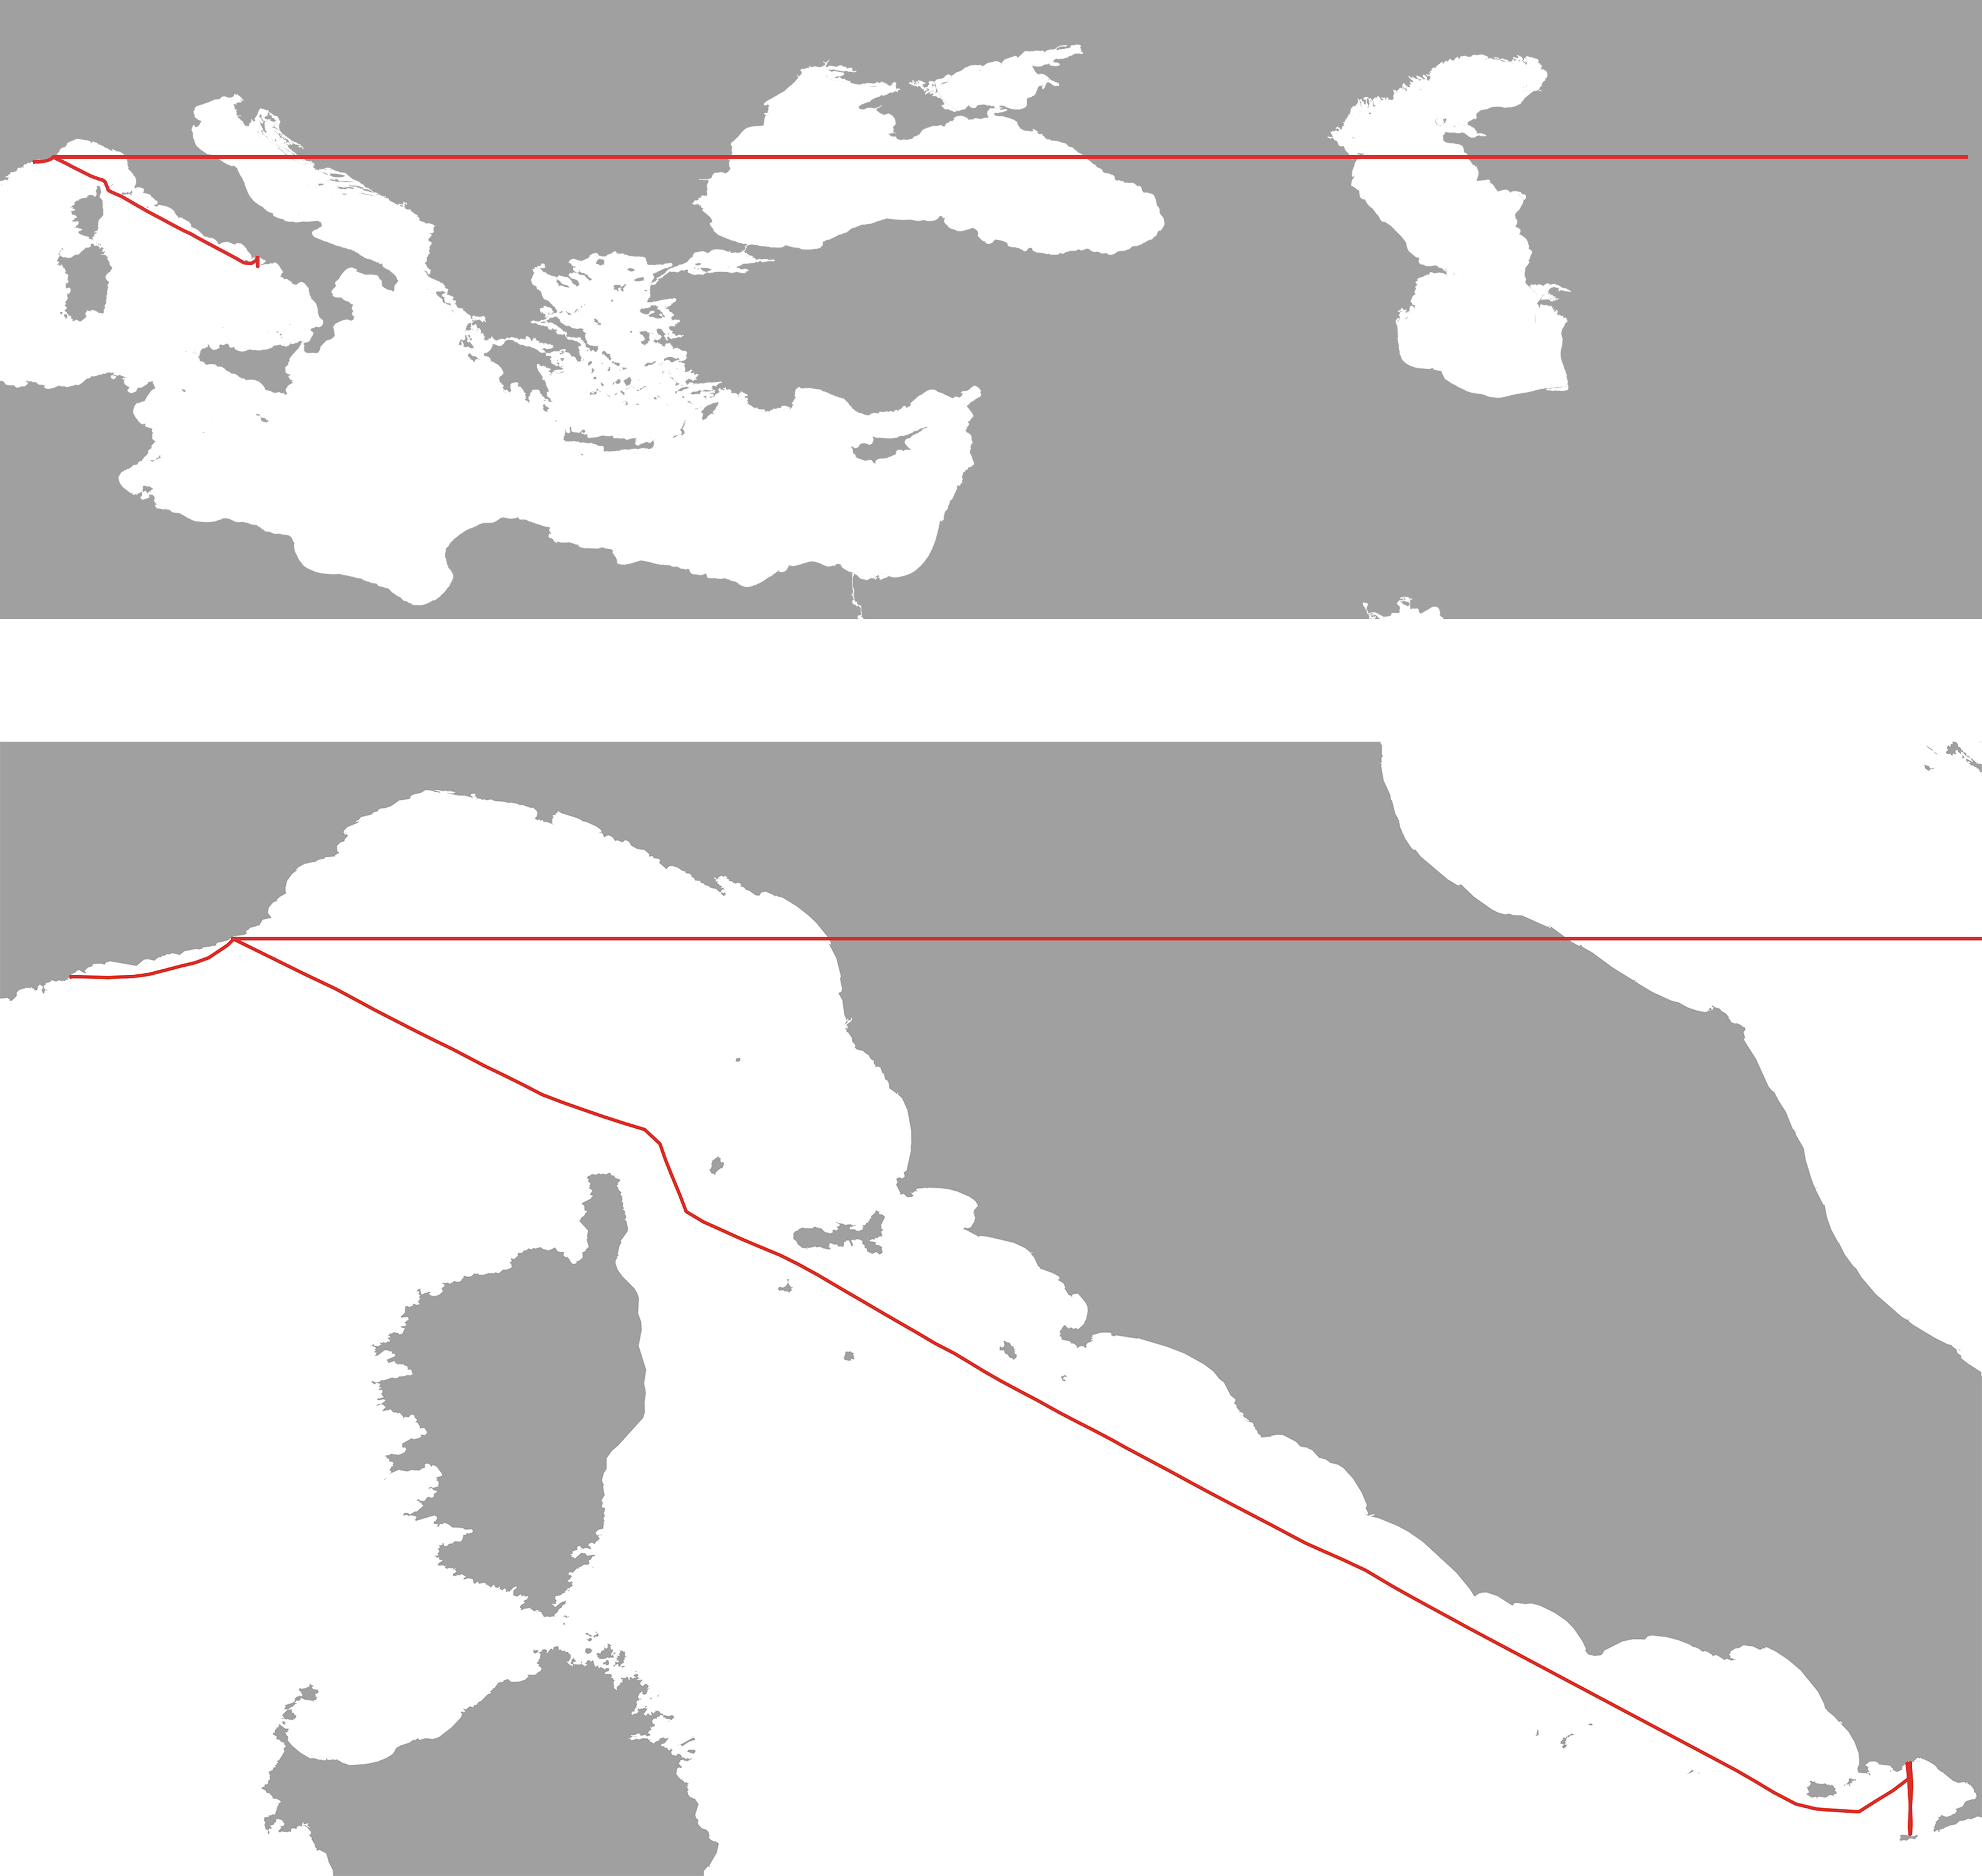
\includegraphics[width=0.7\textwidth]{figures/trajectory_noise/noisy_trajectory}
    \caption{Example showing a ``noisy'' trajectory presumably caused by GPS inaccuracy or equipment error}
    \label{fig:noisy_trajectory}
\end{figure}

An example of this issue is visualized in \cref{fig:noisy_trajectory} which shows a voyage starting in Monaco and ending in Naples, Italy. During a stopping point in northern Italy, the vessel transmitted two longitude values placing the vessel in the middle-east while then continuing the journey arriving in Naples, Italy. This issue is presumably caused by issues with the GPS signals sent by the \acrshort{ais} transmitter on board the vessel or by some other equipment error. Excluding the fluctuated segment of the trajectory, the remaining trajectory is completely valid, thus, if it is possible to remove the invalid part of the trajectory, the remainder could be further used in the analysis. Therefore, ``noise filter'' was employed to detect and cut away fluctuations in otherwise valid trajectories.

\begin{figure}[htbp]  % order of priority: h here, t top, b bottom, p page
    \centering
    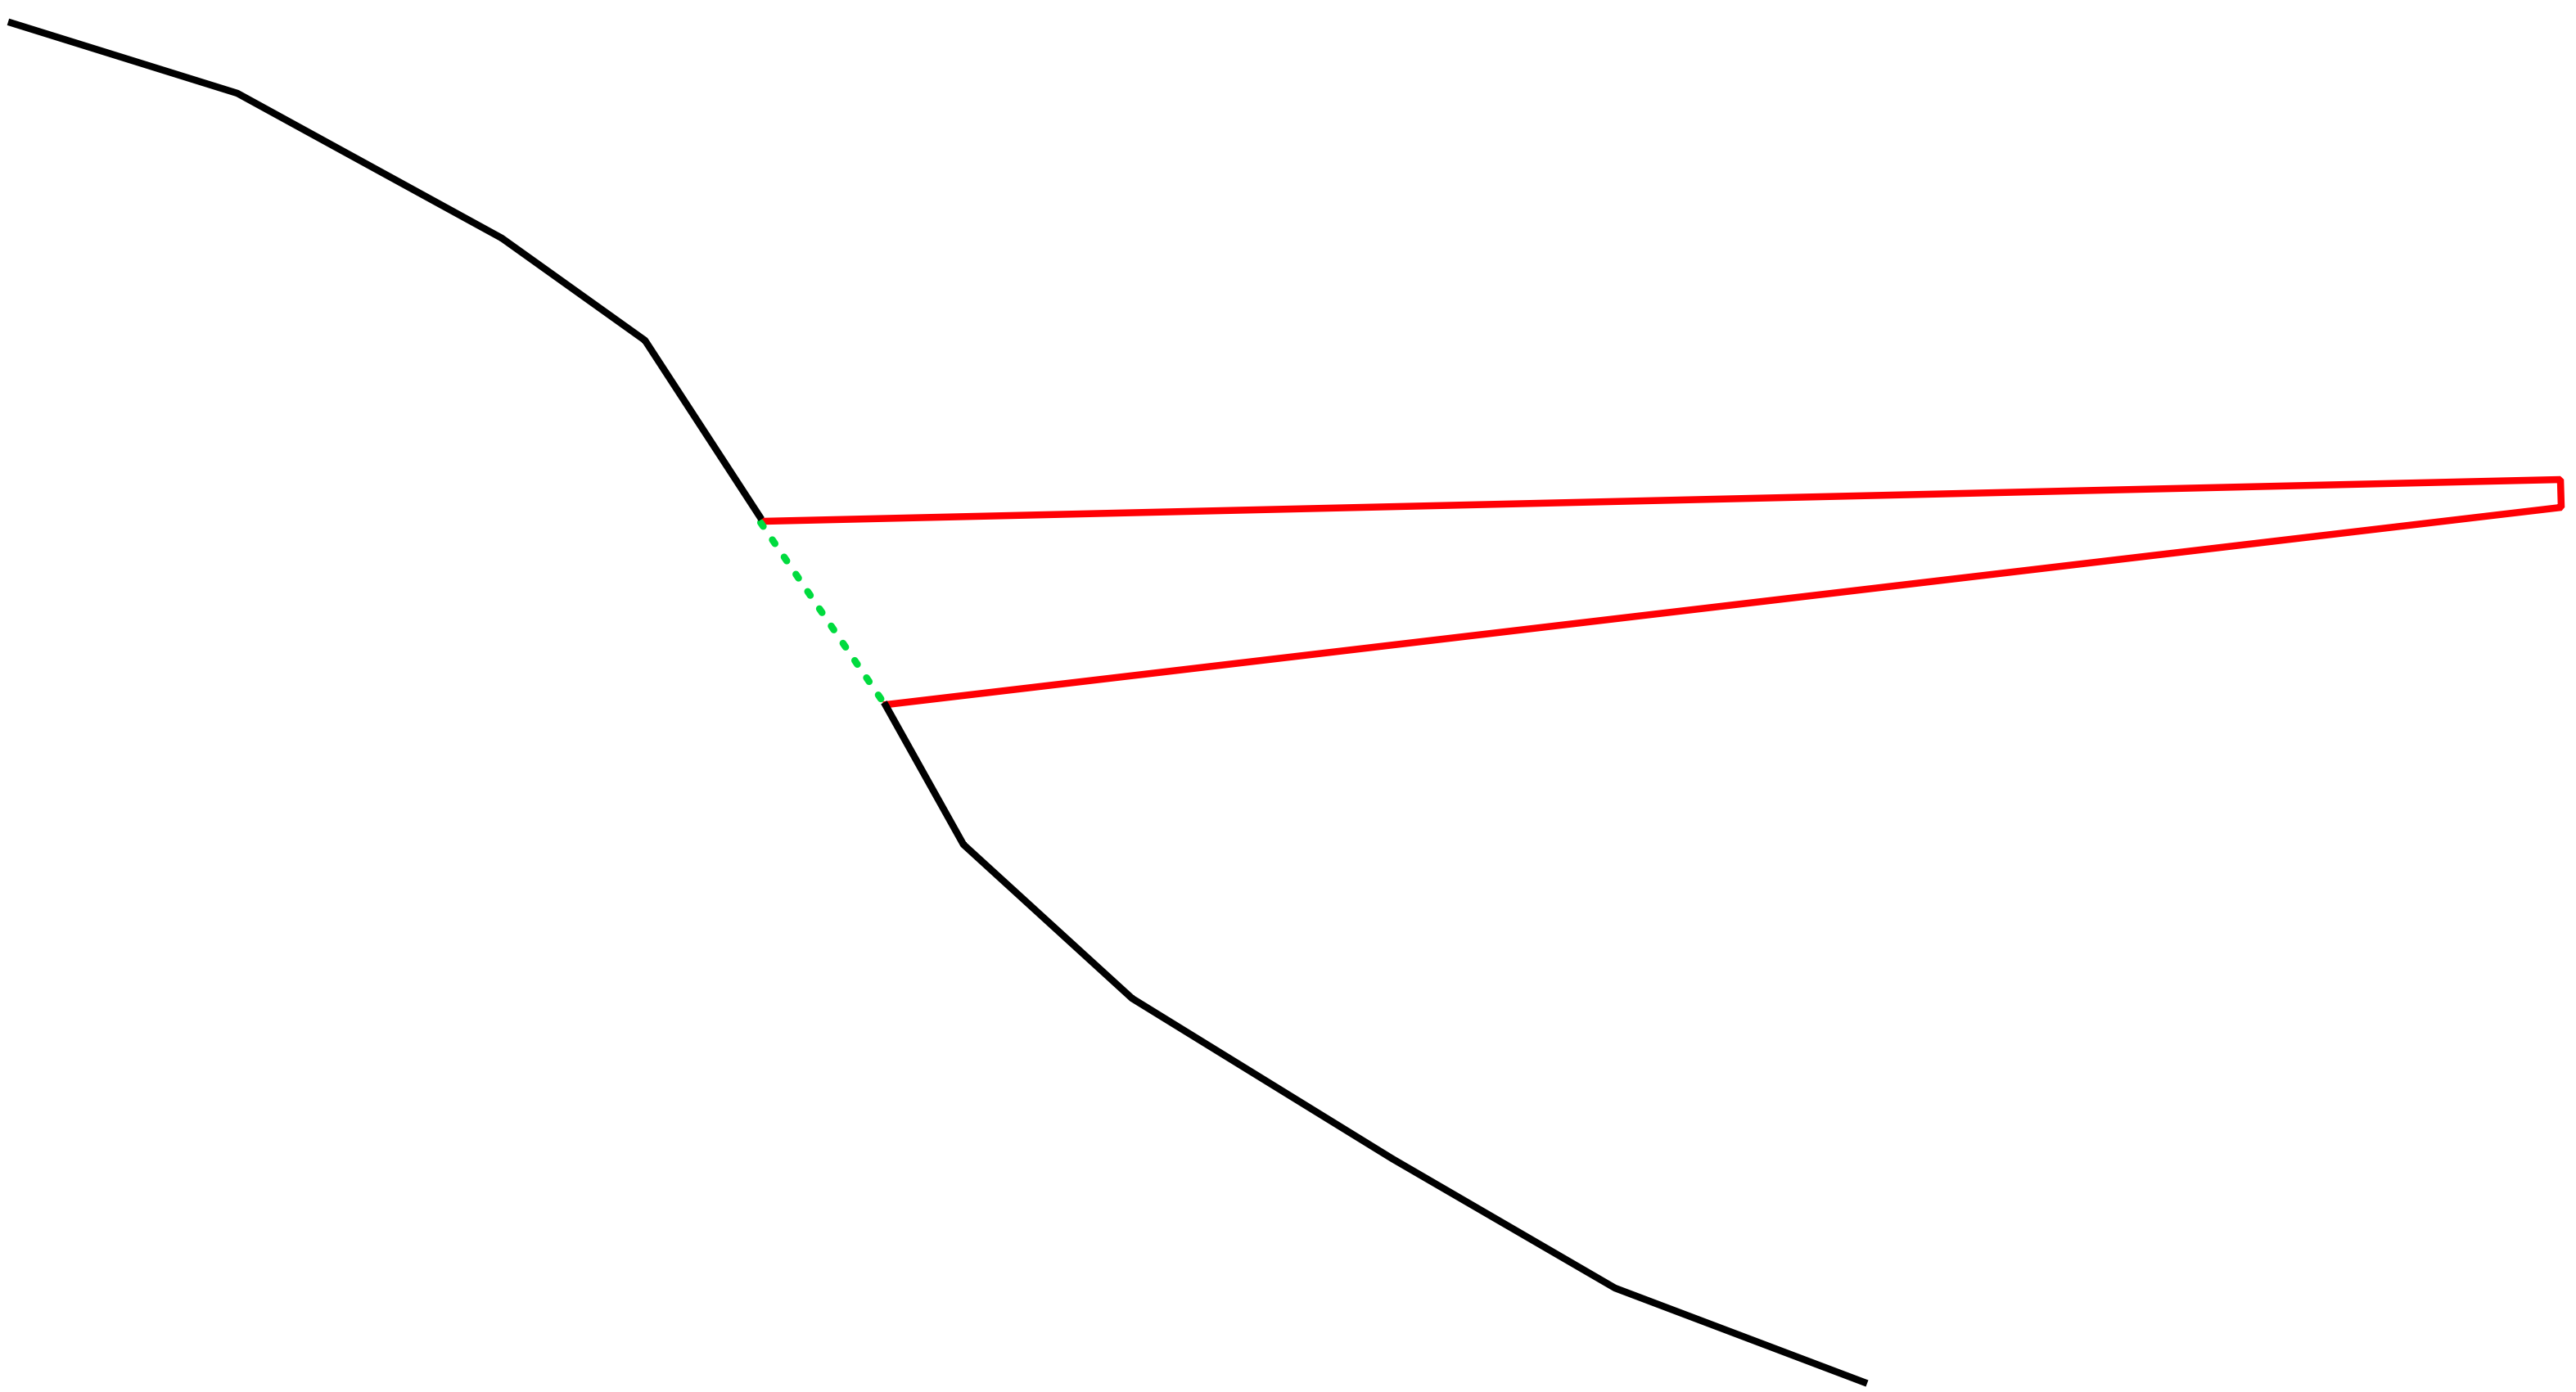
\includegraphics[width=0.6\textwidth]{figures/trajectory_noise/noise_filter}
    \caption{Noise filter algorithm cutting out points in a trajectory detected as noise. The red segment is cut out and the black segments are tied together as shown with the green dotted line.}
    \label{fig:noise_filter}
\end{figure}

\begin{figure}[htbp]  % order of priority: h here, t top, b bottom, p page
    \centering
    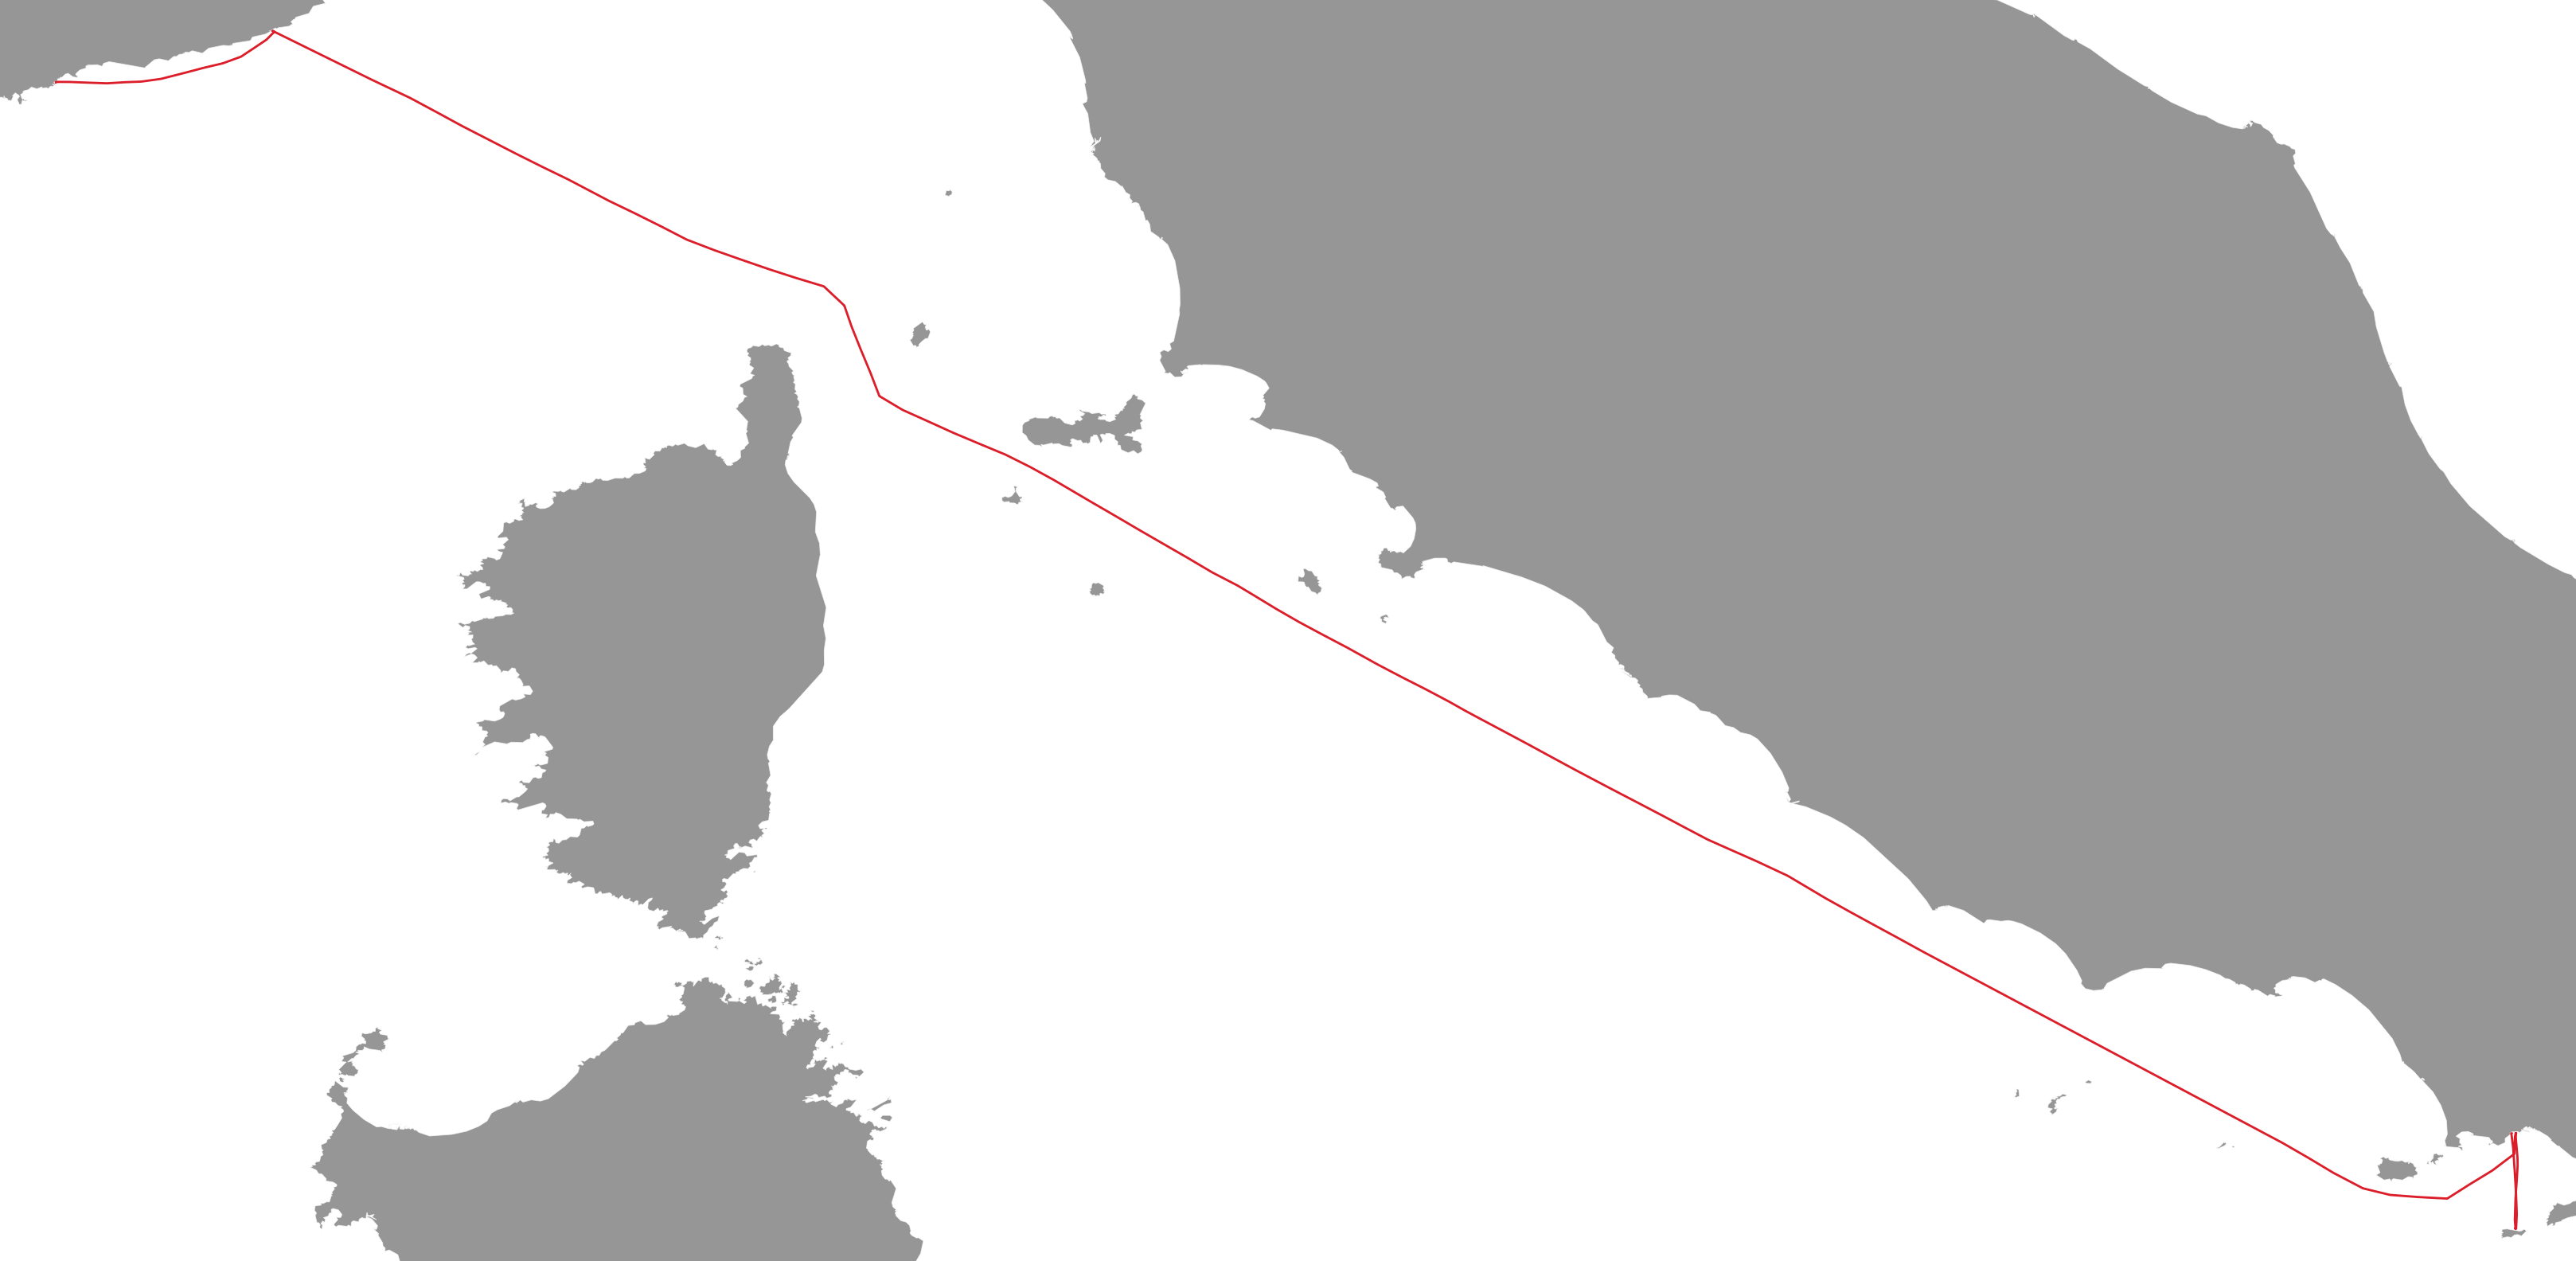
\includegraphics[width=0.8\textwidth]{figures/trajectory_noise/filtered}
    \caption{The example trajectory shown \cref{fig:noise_filter} from Monaco to Naples after noise filtering.}
    \label{fig:noise_filtered}
\end{figure}

The noise filtering employed in the trajectory builder is shown in \cref{fig:noise_filter} where the red segment fluctuates in an otherwise valid trajectory and is therefore excluded from the remaining trajectory. For every point in the trajectory, the algorithm checks the distance between the current and the next point as well as the time difference between the two points. Using the distances in space and time, it calculates the speed the vessel would require to travel from the first to the second point. If the speed required was more than 50 knots, the segment was invalid. The next point is then compared to the first to see if there is a possible valid path to the third point. If there is, the second point is disregarded from the trajectory. The algorithm is given a tolerance of four invalid points before it disregards the entire trajectory. \cref{lst:noise_filter} shows the function used to find the next valid point in a trajectory, if it returns an error, the trajectory is disregarded. \cref{fig:noise_filtered} shows the same trajectory from \cref{fig:noisy_trajectory} after the following algorithm has filtered out fluctuating segments.

\begin{lstlisting}[
    caption={Golang code used find the next valid point for any given point in a trajectory.},
    label=lst:noise_filter,
    language=Go
]
// nextValidPoint returns the index of the next valid point checking distances to
// every point within tolerance. If no valid distances were found wihin tolerance,
// it returns an error. If the last point in trajectory was reached, -1 is returned
func nextValidPoint(start, tolerance int, positions []VesselPosition) (int, error) {
	a := positions[start]
	for j := start + 1; j <= start+tolerance; j++ {
		if j >= len(positions) {
			return -1, nil
		}

		n := positions[j]
		dist := DistanceHaversine(Point{a.Lon, a.Lat}, Point{n.Lon, n.Lat})
		// use the absolute value in case the trajecotory is not sorted
		timeDiff := math.Abs(float64(n.Timestamp - a.Timestamp))

		// calculate the required speed to reach the given point with the
		// given time difference * 1.94385 to konvert m/s to knots
		requiredSpeed := (dist / timeDiff) * 1.94385
		// if required speed was >= 50kt, move on to next point
		if requiredSpeed < 50.0 {
			return j, nil
		}
	}
	// no reasonable distances were found within tolerance
	return -1, errors.New("trajectory segment too noisy")
}
\end{lstlisting}

Finally, when the voyage trajectories have been constructed and validated, they are collected in a database table called transition voyages which contains the following relevant attributes:

\begin{itemize}
    \item imo - identifier for the vessel.
    \item mmsi - identifier for the vessel.
    \item departure port - voyage departure port's locode.
    \item departure timestamp - the time of departure.
    \item arrival port - voyage arrival port's locode.
    \item arrival timestamp - the time of arrival.
    \item trajectory - 3D linestring with longitude, latitude, and timestamp for each point.
\end{itemize}

It is worth noting that the trajectories are stored as 3D PostGIS linestring geometries where each point contains a \textit{x}, \textit{y}, and \textit{z} value where the \textit{z} value holds the UNIX timestamp of the positional record. Keeping the timestamp value is necessary for sampling trajectories based on time, and keeping the time values stored directly in the trajectory geometry saves an extra table for trajectory points.

\section{Data processing for \acrfull{ml}}

After the initial data set has been collected and vessel voyages have been defined and constructed, the next step is to build the final training dataset to be used for analysis and \acrfull{ml}. This section describes every step in the process used to construct this dataset based on data described up to this point in this chapter.

\subsection{Trajectory sampling}

Vessels transmit \acrshort{ais} records at different frequencies and messages collected via satellite are collected at different frequencies as the satellites have different orbits. Therefore the frequency, or density, or records in trajectories can not be expected to be standardized. Furthermore, as vessels travel at different speeds, two trajectories with similar start and end positions might have different shapes and contain a different number of points. In addition, as discussed in \cref{sec:vessel_voyage_definition}, one disadvantage of relying on \acrshort{ais} navigational statuses is that vessels can stop during a voyage for different reasons before arriving at their final destinations. Whenever a vessels stops moving or moves slowly, many \acrshort{ais} records are transmitted in clusters which cause noise and redundant data in the constructed trajectories.

\begin{figure}[htbp]  % order of priority: h here, t top, b bottom, p page
    \centering
    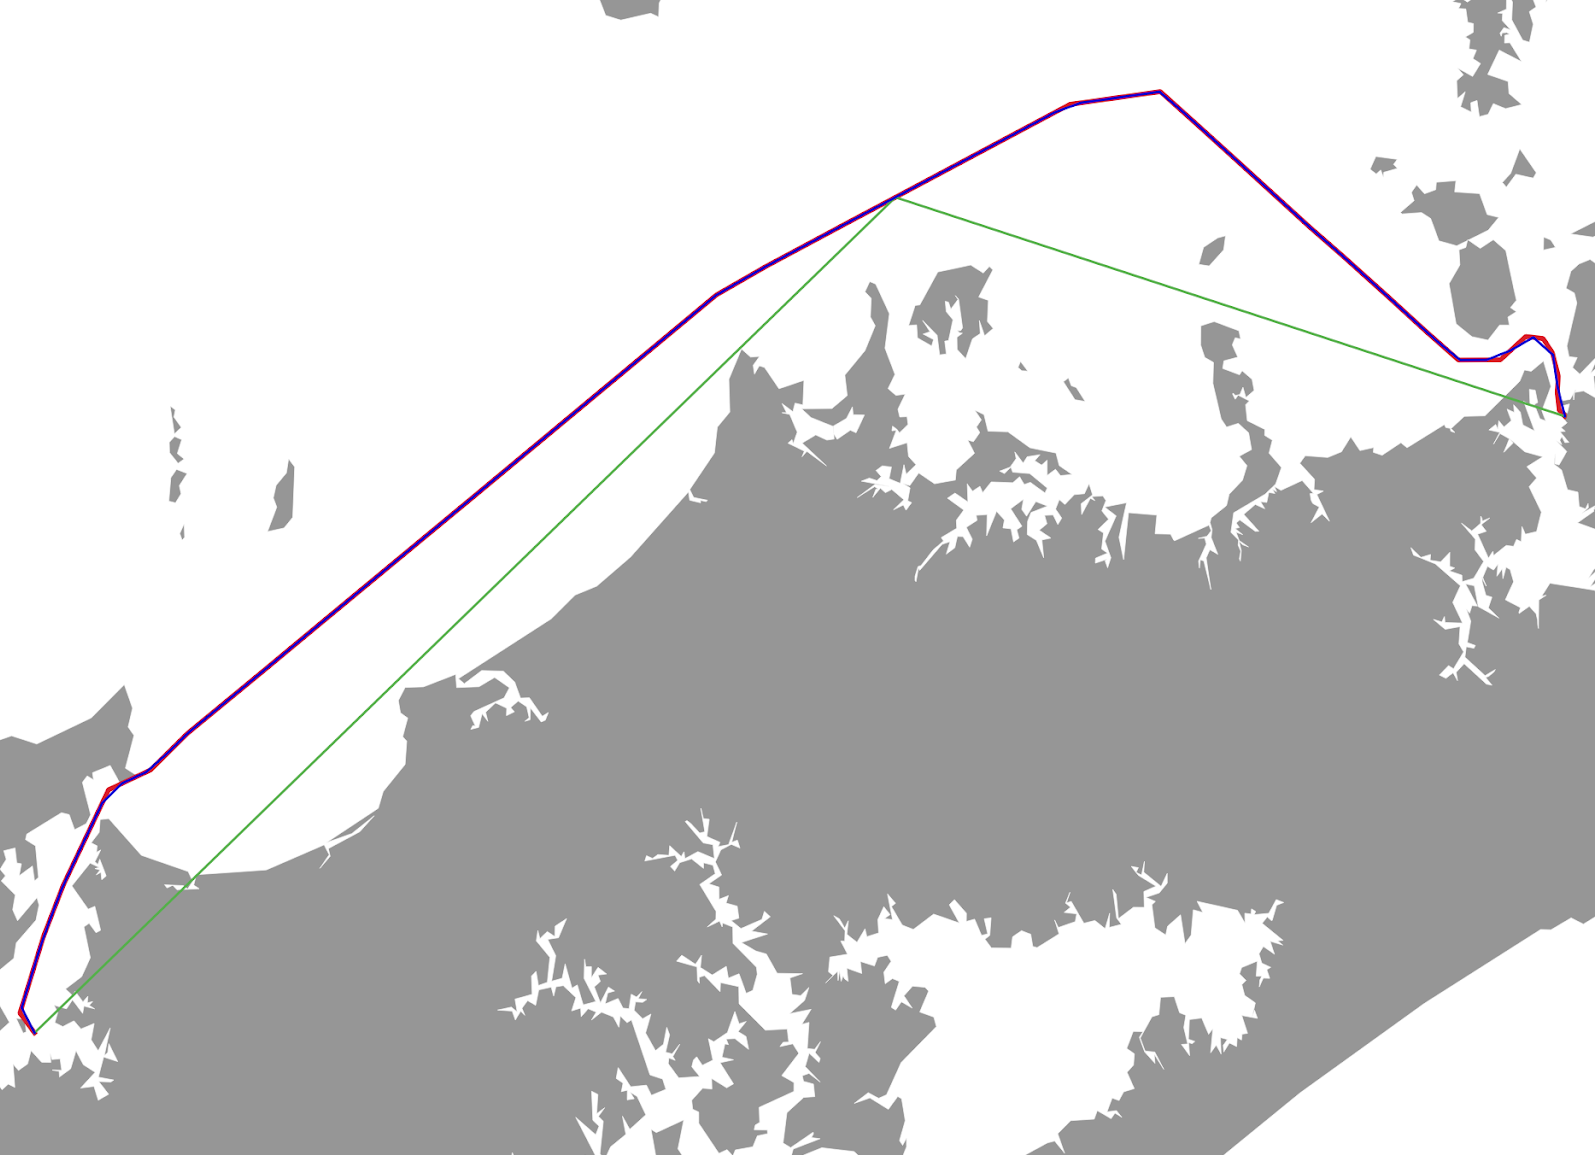
\includegraphics[width=0.8\textwidth]{figures/trajectory_sampling}
    \caption{Example of a trajectory sampled by both distance (2 km) and time (6 hours). The red trajectory is not sampled, the blue is sampled based on 2 km in distance, and the green is sampled based on six hour time intervals.}
    \label{fig:trajectory_sampling}
\end{figure}

The proposed solution includes using similarity between trajectories to predict traveling vessels' destination ports, therefore, in order to make the trajectories more comparable a sampling step was added in the process of constructing the training data. There were two main approaches considered for trajectory re-sampling, namely sampling based on distance and time. When sampling based on a predefined distance, each subsequent point in a trajectory must be the same distance apart from each other. When sampling based on time, one position is extracted from a trajectory for every given unit of time. For instance, if sampling based on time with a six hour sample rate, starting from the first point, every position within six hour intervals are grouped and all positions within each group are dropped except for the first one. Both methods achieve the goal of making trajectories more comparable, however, sampling based on time simplifies, or reduces, the amount of data in each trajectory the most. It also provides an indication of trajectory duration implicitly through the trajectory length, or the number of points in a trajectory.

For these reasons, throughout the rest of the implementation, sampling is done based on time using a time interval of six hours. It is worth noting that for trajectories shorter than six hours, only the first and last point in the trajectory is returned reducing the trajectory to a straight line. In order to sample any trajectory based on either time or distance, a Golang package was written called ``sampler'' which can parse and handle both 3D trajectories including timestamps for time sampling, and 2D trajectories for distance sampling. The complete code for this package can be found in \cref{app:sampler}. \cref{lst:trajectory_sampler} shows an extract from this package of the function used to resample trajectories based on time.

\begin{lstlisting}[
    caption={Golang code from a sampler package written to sample a trajectory based on time.},
    label=lst:trajectory_sampler,
    language=Go
]
// resampleTime resamples trajectory based on s.SampleRate given in hours.
// Extracts the first position within intervals based on sample rate
func (s *Instance) resampleTime() (string, error) {
	var err error
	trajectory, err := s.parse3DTrajectory()
	if err != nil {
		return "", err
	}

	intervals := s.getTimeIntervals(trajectory)
	reducedCoords := []geom.Coord{}
	coords := trajectory.Coords()

	// within each interval add the first coord to reducedCoords
	for _, interval := range intervals {
		var first *geom.Coord

                // get first coord in interval
		for i := range coords {
		        // roundTime uses s.SampleRate when rounding
			coordInterval := s.roundTime(int64(coords[i][2]))
			if coordInterval == interval {
				first = &coords[i]
				break
			}
		}
		if first != nil {
			reducedCoords = append(reducedCoords, *first)
		}
	}

	// if the last coord wasn't the last in reduced, add it
        lastReduced := reducedCoords[len(reducedCoords)-1]
	if !lastReduced.Equal(geom.XYZ, coords[len(coords)-1]) {
		reducedCoords = append(reducedCoords, coords[len(coords)-1])
	}
	if len(reducedCoords) <= 1 {
		return "", errors.New("too few points in sampled trajectory")
	}
	reduced, err := geom.NewLineString(geom.XYZ).SetCoords(reducedCoords)
	if err != nil {
		return "", err
	}

	return geomwkt.Marshal(reduced)
}
\end{lstlisting}

The function listed in \cref{lst:trajectory_sampler} is used in a batch process that samples every voyage's trajectory and keeps the sampled voyages in a separate table called ``sampled transition voyages''. The batch process extracts 5000 voyages at a time, samples their trajectories, and batch-inserts them into the separate table. By not mutating the original voyage data, different sampling methods can be applied and tested to find differences in trajectory comparisons.

\subsection{\acrfull{mstd}}

In order for the proposed solution to take into account both geographical trajetories as well as additional vessel information for predictions, in the training set, the trajectories have been abstracted into the categorical and numeric values \acrfull{mstd}, the similarity value for the \acrshort{mstd}, and then the length of the trajectory. The \acrshort{mstd} for a given voyage is found by measuring the similarity between the given voyage's trajectory and every historical trajectory in the sampled transition voyages table. The most similar trajectory is found using a given trajectory similarity measurement, and its destination and similarity value is added to the final dataset. As described in \cref{sec:trajectory_similarity}, there are several different trajectory similarity measurements available, however, for this thesis the \acrfull{sspd} is used to calculate the \acrshort{mstd} values. However, the process and the dataset is structured in such a way that it is possible to use different similarity measurement methods in this process. For instance, the \acrshort{ml}-based method proposed in \cite{Zhang2020AISApproach} achieved good performance for similarity based predictions, thus it could be replicated and used to calculate the \acrshort{mstd} values for this approach.

\begin{figure}[htbp]  % order of priority: h here, t top, b bottom, p page
    \centering
    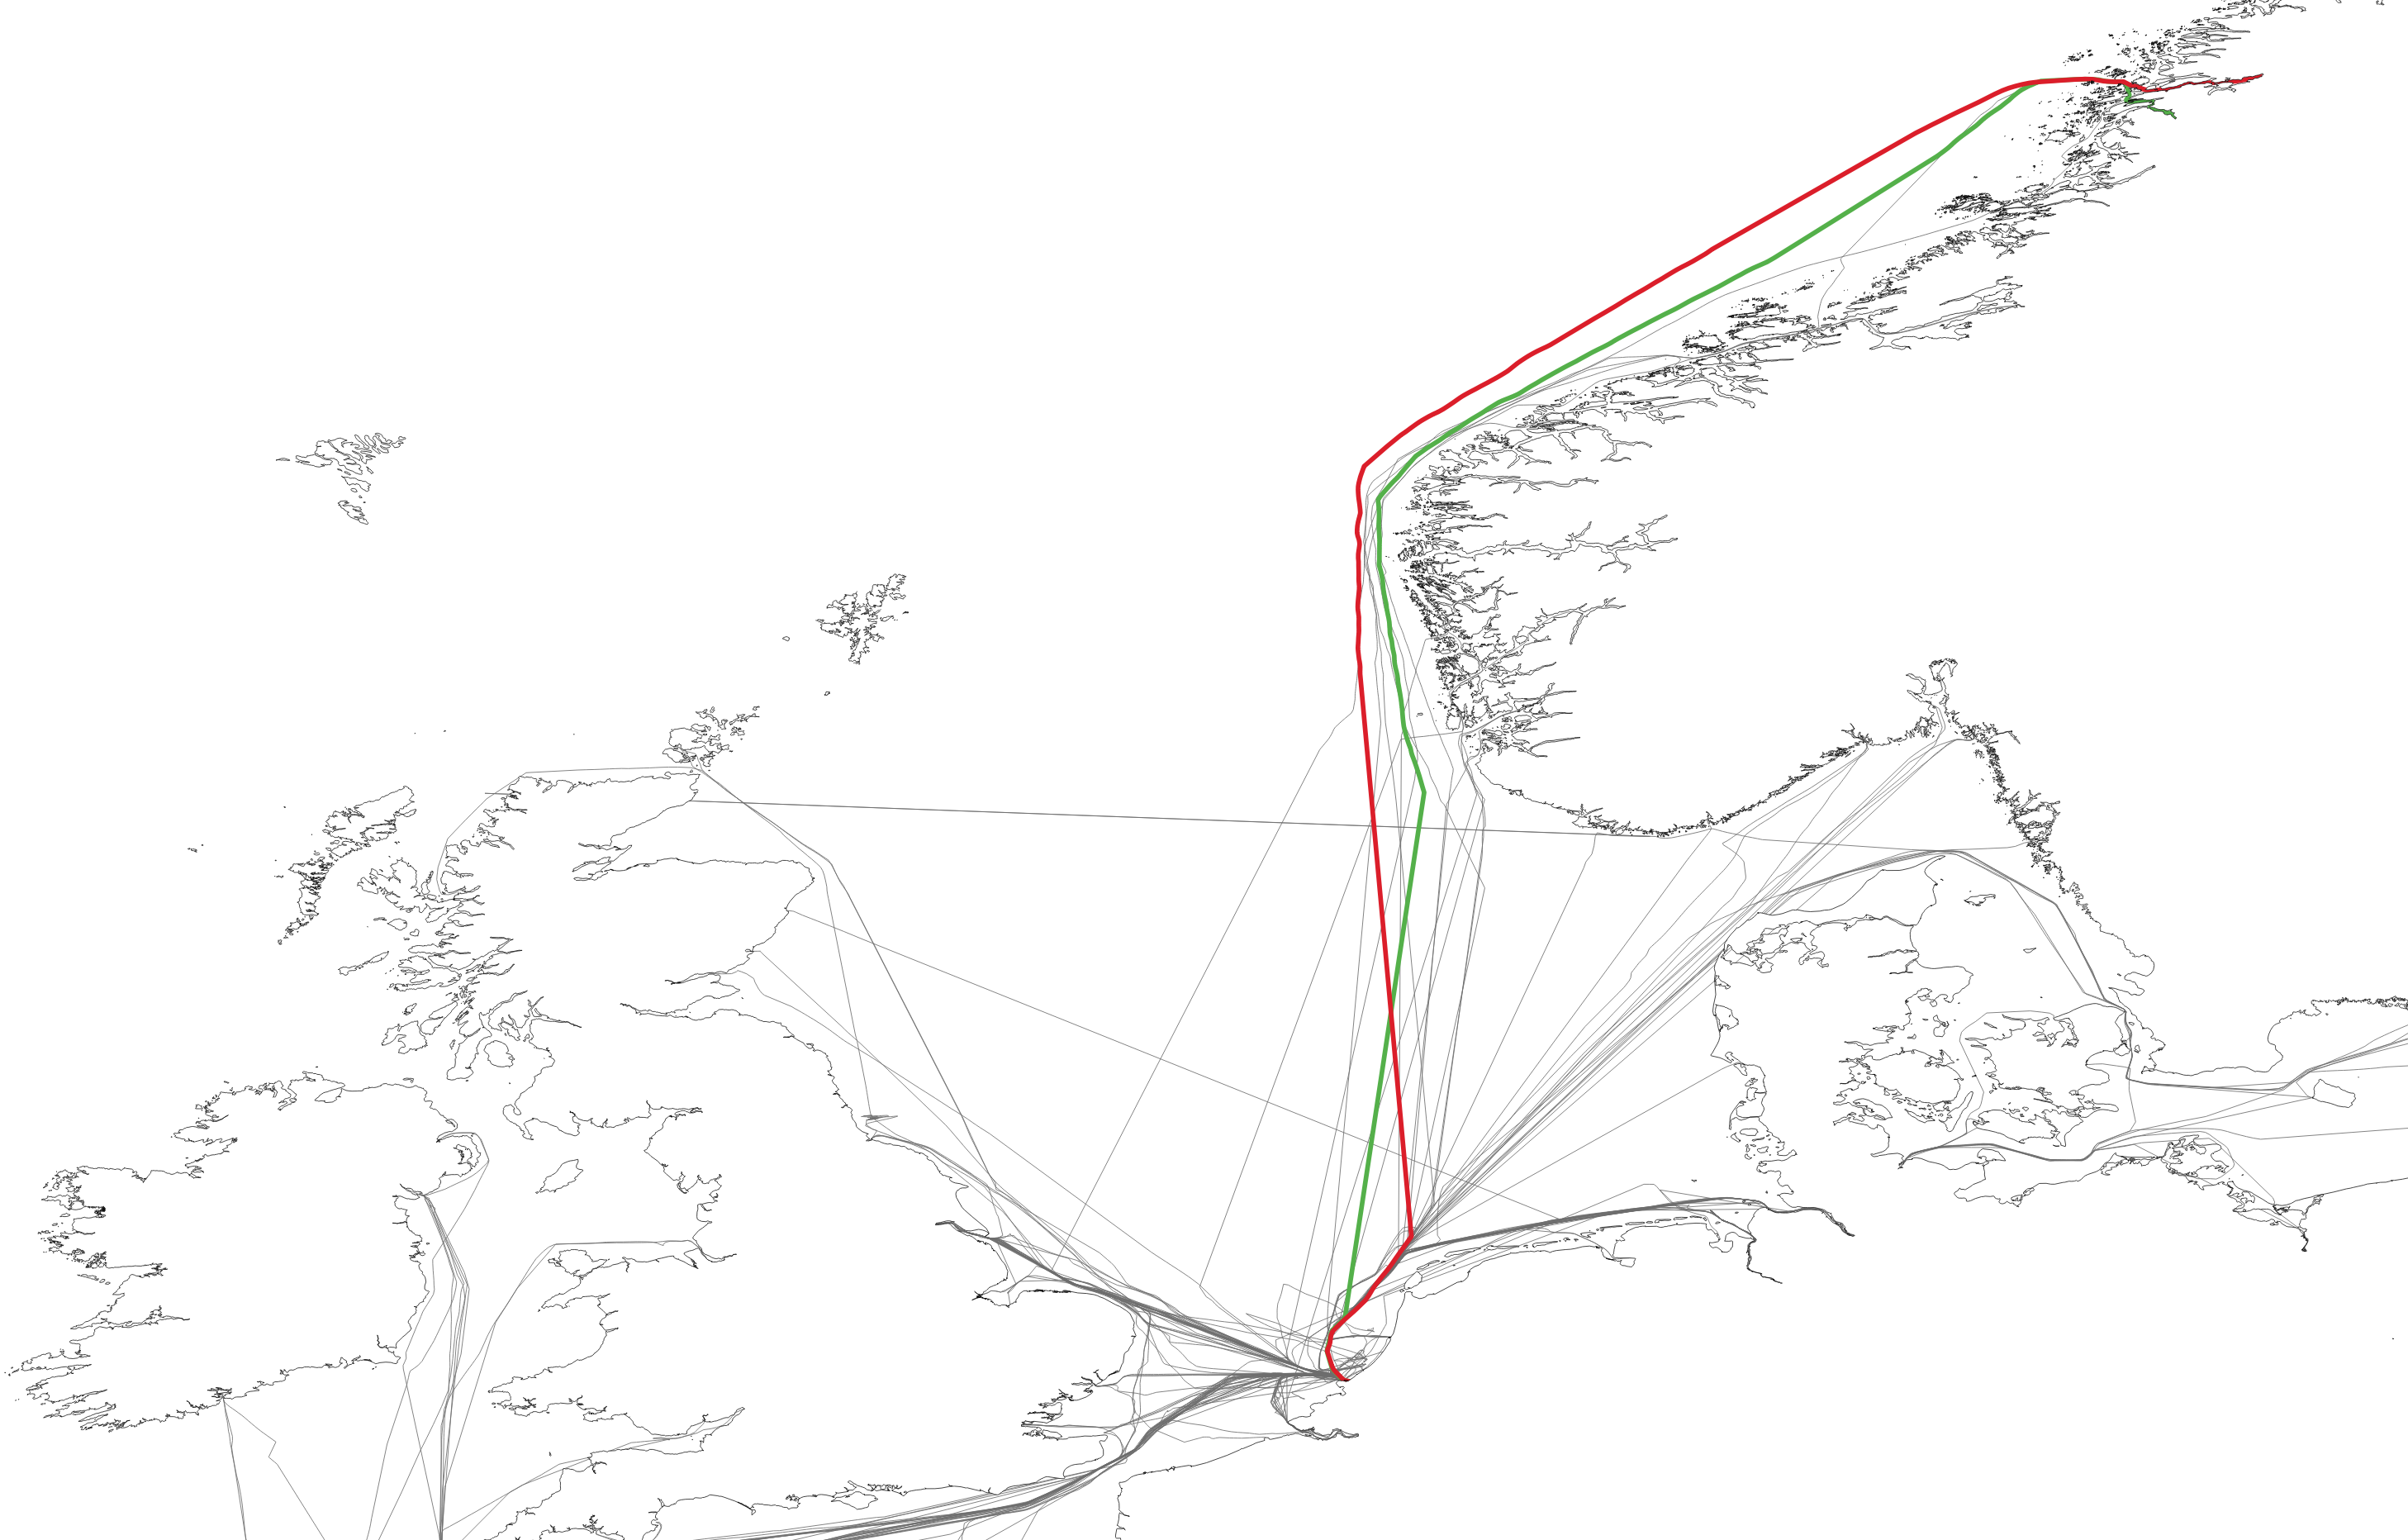
\includegraphics[width=1.0\textwidth]{figures/mstd}
    \caption{Example of \acrshort{mstd} for a given historical trajectory where the red line is the given trajectory and the green line is the most similar historical trajectory.}
    \label{fig:mstd}
\end{figure}

The \acrshort{mstd} value for a given voyage is calculated in the following steps:

\begin{enumerate}
    \item Given a sampled voyage, fetch every historical voyage with the same departure port from vessels of the same segment and sub-segment.
    \item Use a given similarity measurement method, \acrshort{sspd} in this case, to calculate the similarity between the given voyage's trajectory and every historical voyage's trajectory. The given similarity measurement method must return a similarity value. For \acrshort{sspd}, this value is a Haversine distance value.
    \item Find the most similar historical trajectory, or the trajectory with the smallest similarity value.
    \item Extract the most similar historical trajectory's destination port as the \acrshort{mstd} value and extract the similarity value for future use.
\end{enumerate}

\cref{fig:mstd} shows an example of finding the most similar historical trajectory (green line) for a given voyage (red line). The given voyage departed the port of Rotterdam, and arrived in Mo i Rana, Norway. Every other historical voyage that departured Rotterdam from vessels of the same segment and sub-segment was then extracted and \acrshort{sspd} was used to find the most similar historical trajectory.

\subsection{Building ML data training set}

\begin{itemize}
    \item Batch calculating MSTD with incomplete voyages
    \item Different trajectory similarity approaches
    \item Adding more data attributes per voyage such as seasons, ballast/laden, etc\ldots
    \item Final result/structure
\end{itemize}

\subsection{Dataset imbalance}

\begin{itemize}
    \item Minority oversampling
    \item Majority undersampling
\end{itemize}

\subsection{Categorical label encoding}

\begin{itemize}
    \item Categorical values/labels must be encoded
    \item Label encoding vs one-hot encoding
\end{itemize}

\section{The final dataset summary}

The final process of creating the dataset used in the analysis can be summarized in the following steps:

\begin{itemize}
    \item Voyages are defined using time intervals provided by the vessels' \acrshort{ais} navigational status. They are constructed and stored in a voyage database table containing the full geographical trajectory, arrival and departure ports, and additional information for the traveling vessel.
    \item The voyage table's geographical trajectories are sampled, or simplified, based on a certain time interval to make trajectory comparisons easier.
    \item Every sampled historical trajectory is split into multiple parts to emulate incomplete voyages not yet arrived at a port. Furthermore, the \acrshort{mstd} is calculated for every one of these voyages. Trajectory similarity is defined using the \acrshort{sspd} algorithm, however, this data is interchangeable with other similarity measurements.
    \item Finally, the \acrshort{mstd}, similarity value, trajectory length, departure and arrival ports, and vessel segmentation information is collected and stored as the \acrshort{ml} training data.
\end{itemize}

An overview of the process described in this chapter thus far is shown in \cref{fig:dataset_overview} from the data provided by \acrfull{mo} to the final \acrshort{ml} training data.

\begin{figure}[htbp]  % order of priority: h here, t top, b bottom, p page
    \centering
    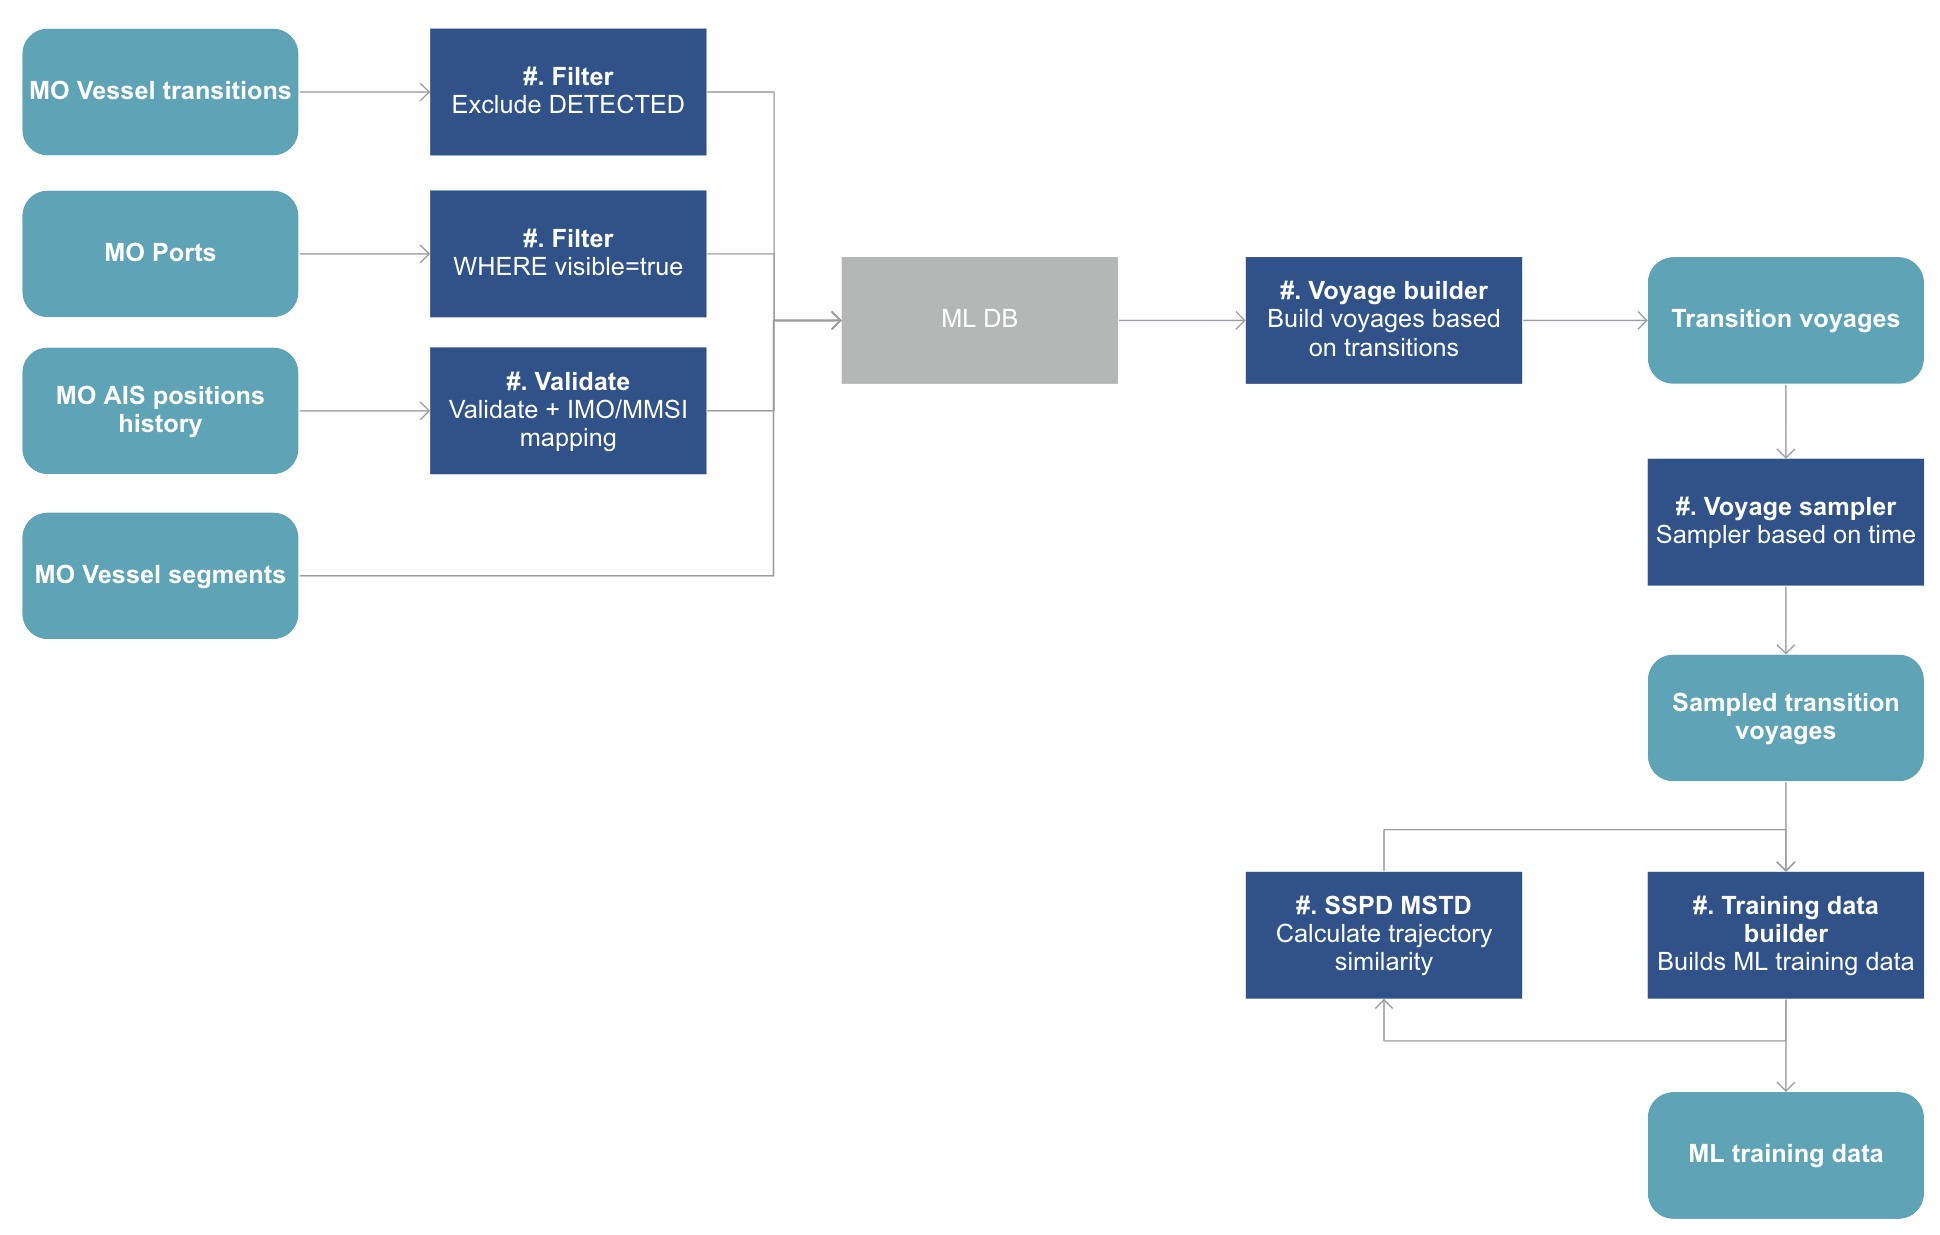
\includegraphics[width=1.0\textwidth]{figures/dataset_overview}
    \caption{Overview of the process used to construct the dataset used in further analysis and \acrshort{ml}.}
    \label{fig:dataset_overview}
\end{figure}

The final dataset is collected in a database table called \acrshort{ml} training data, and it contains the following attributes:

\begin{table}[htbp]
    \centering
    \begin{tabularx}{1.0\textwidth}{p{1.0in} p{0.75in} X}
    \hline
        \bfseries{Column} & \bfseries{Type} & \bfseries{Description} \\ \toprule
        id & serial int & unique identifier \\ \midrule
        voyage\_id & int & the original voyage id from sampled transition voyages \\ \midrule
        imo & int & identifier for the traveling vessel\\ \midrule
        mmsi & int & identifier for the traveling vessel\\ \midrule
        segment & string & the vessel's segment \\ \midrule
        sub\_segment & string & the vessel's sub-segment \\ \midrule
        departure\_port & string & \gls{locode} of the vessel's departure port \\ \midrule
        trajectory\_length & int & number of points in the sampled trajectory \\ \midrule
        sspd\_mstd & string & \gls{locode} of the \acrshort{mstd} value for the voyage trajectory \\ \midrule
        sspd\_dist & int & similarity value between the voyage trajectory and the most similar historical trajectory   \\ \midrule
        arrival\_port & string & \gls{locode} of the vessel's arrival port \\ \bottomrule
    \end{tabularx}
\caption{Final structure of the ml\_training\_data database table.}\label{tab:ml_training_data}
\end{table}




\section{ML-based training and destination prediction}

\subsection{Model selection}

\begin{itemize}
    \item Tree-based classifiers
    \item Multi-layered perceptrons classifiers
    \item Support-vector machines
    \item Multi-class classifiers vs OneVsRest binary classifiers
\end{itemize}

\subsection{Configuration and parameter optimization}

\subsection{Training}

\subsection{Evaluation process and metrics}

\begin{itemize}
    \item X-Folder-cross-validation
    \item Metrics: F1, precision, recall, AUC, vs accuracy
    \item Computing performance?
    \item How fast is it to compute the next destination of every vessel in the world
\end{itemize}

\section{Vessel destination prediction method summary}

Given the final trained model, the overall prediction process for a single traveling vessel can be conceptualized using the following steps:

\begin{itemize}
    \item The current trajectory of the traveling vessel is collected using \acrshort{ais} records ranging from the last transmitted \textit{``MOORED''} status to its current position along with the id (\gls{locode}) of the departure port where it was moored and the vessel's segmentation values.
    \item The vessel's trajectory is then sampled based on a predefined time interval, then compared to every historical outgoing trajectory from the same departure port from vessels of the same segment and sub-segment to establish the \acrfull{mstd}.
    \item The vessel's segment, sub-segment, departure port, trajectory length, \acrshort{mstd}, and the \acrshort{mstd} similarity value is then passed to a \acrshort{xgb} model that predicts the traveling vessel's arrival port.
\end{itemize}

\chapter{Results}
\label{chap:results}

In this section, the results from the proposed solution is described in detail. It describes different results from the different stages throughout the develop process and presents the final results and metrics from the trained \acrfull{ml} model.

\section{Constructed dataset and ML problem formulation}

The initial dataset was copied and validated from \acrfull{mo}'s \acrshort{ais} database. The database table \textit{``vessel\_positions\_history''} was last updated in March 2021 and consists of \textbf{1.2} billion positional \acrshort{ais} records. Each vessel that transmitted positions belongs to a given segment and sub-segment that was made available by the \textit{``vessel\_segment''} table which contains \textbf{eight} different segment values, and \textbf{107} different combinations of segments and sub-segments. The provided \textit{``ports''} data contains \textbf{5200} ports world-wide that all follows the \gls{locode} naming standard. In total, as of March 2021, there were \textbf{6.4} million vessel transitions in the \textit{``vessel\_transitions''} table which was used to construct voyages. This data formed the initial data foundation for the final processed \acrfull{ml} training dataset. All the data that was copied and processed from \acrshort{mo}'s databases were processed in batches. Ports, segments, and transitions where quickly copied and processed, however, the \textbf{1.2} billion positional records took several days to migrate and validate. This was mostly because of the time required to validate coordinates and correctly map \acrshort{mmsi} and \acrshort{imo} values. Throughout this process, the latest identifiers and timestamps were fetched from the dedicated project database to only update data that occurred after the latest records already processed. In this way, this process was idempotent so that running the process multiple times did not affect existing data. This made the system simple to update throughout the development process and as many records as possible were used in the final approach only limited by the thesis time limitation.

\subsection{Voyage definition and construction}

Based on the initial \textbf{6.4} million vessel transitions, \textbf{1.7} million voyages where initially constructed by finding positional records transmitted from a vessel between subsequent departure and arrival transitions. The resulting voyages were, therefore, defined based on transitioning \acrshort{ais} statuses that indicate the vessel is moored or moving. As a consequence of this definition, the quality of the resulting trajectories are very much affected by how well the \gls{aivdm} protocol is followed by the traveling vessels. Since the navigational status attribute is manually inputted by the vessel's captain or crew, the resulting trajectories are prone to human error but results in more complete voyages disregarding intermediate stops for purposes such as bunkering.

As an example, \cref{fig:transition_voyage} shows a voyage from China to Argentina where the vessel stopped at Singapore, most likely to bunker. In the chosen voyage definition, the beginning and end of the voyage is defined based on input from the vessel's captain which results in a voyage starting from China, and ending in Argentina. Further implications and consequences of the chosen definition is later discussed in \cref{chap:discussion}.

\begin{figure}[htbp]
    \centering
    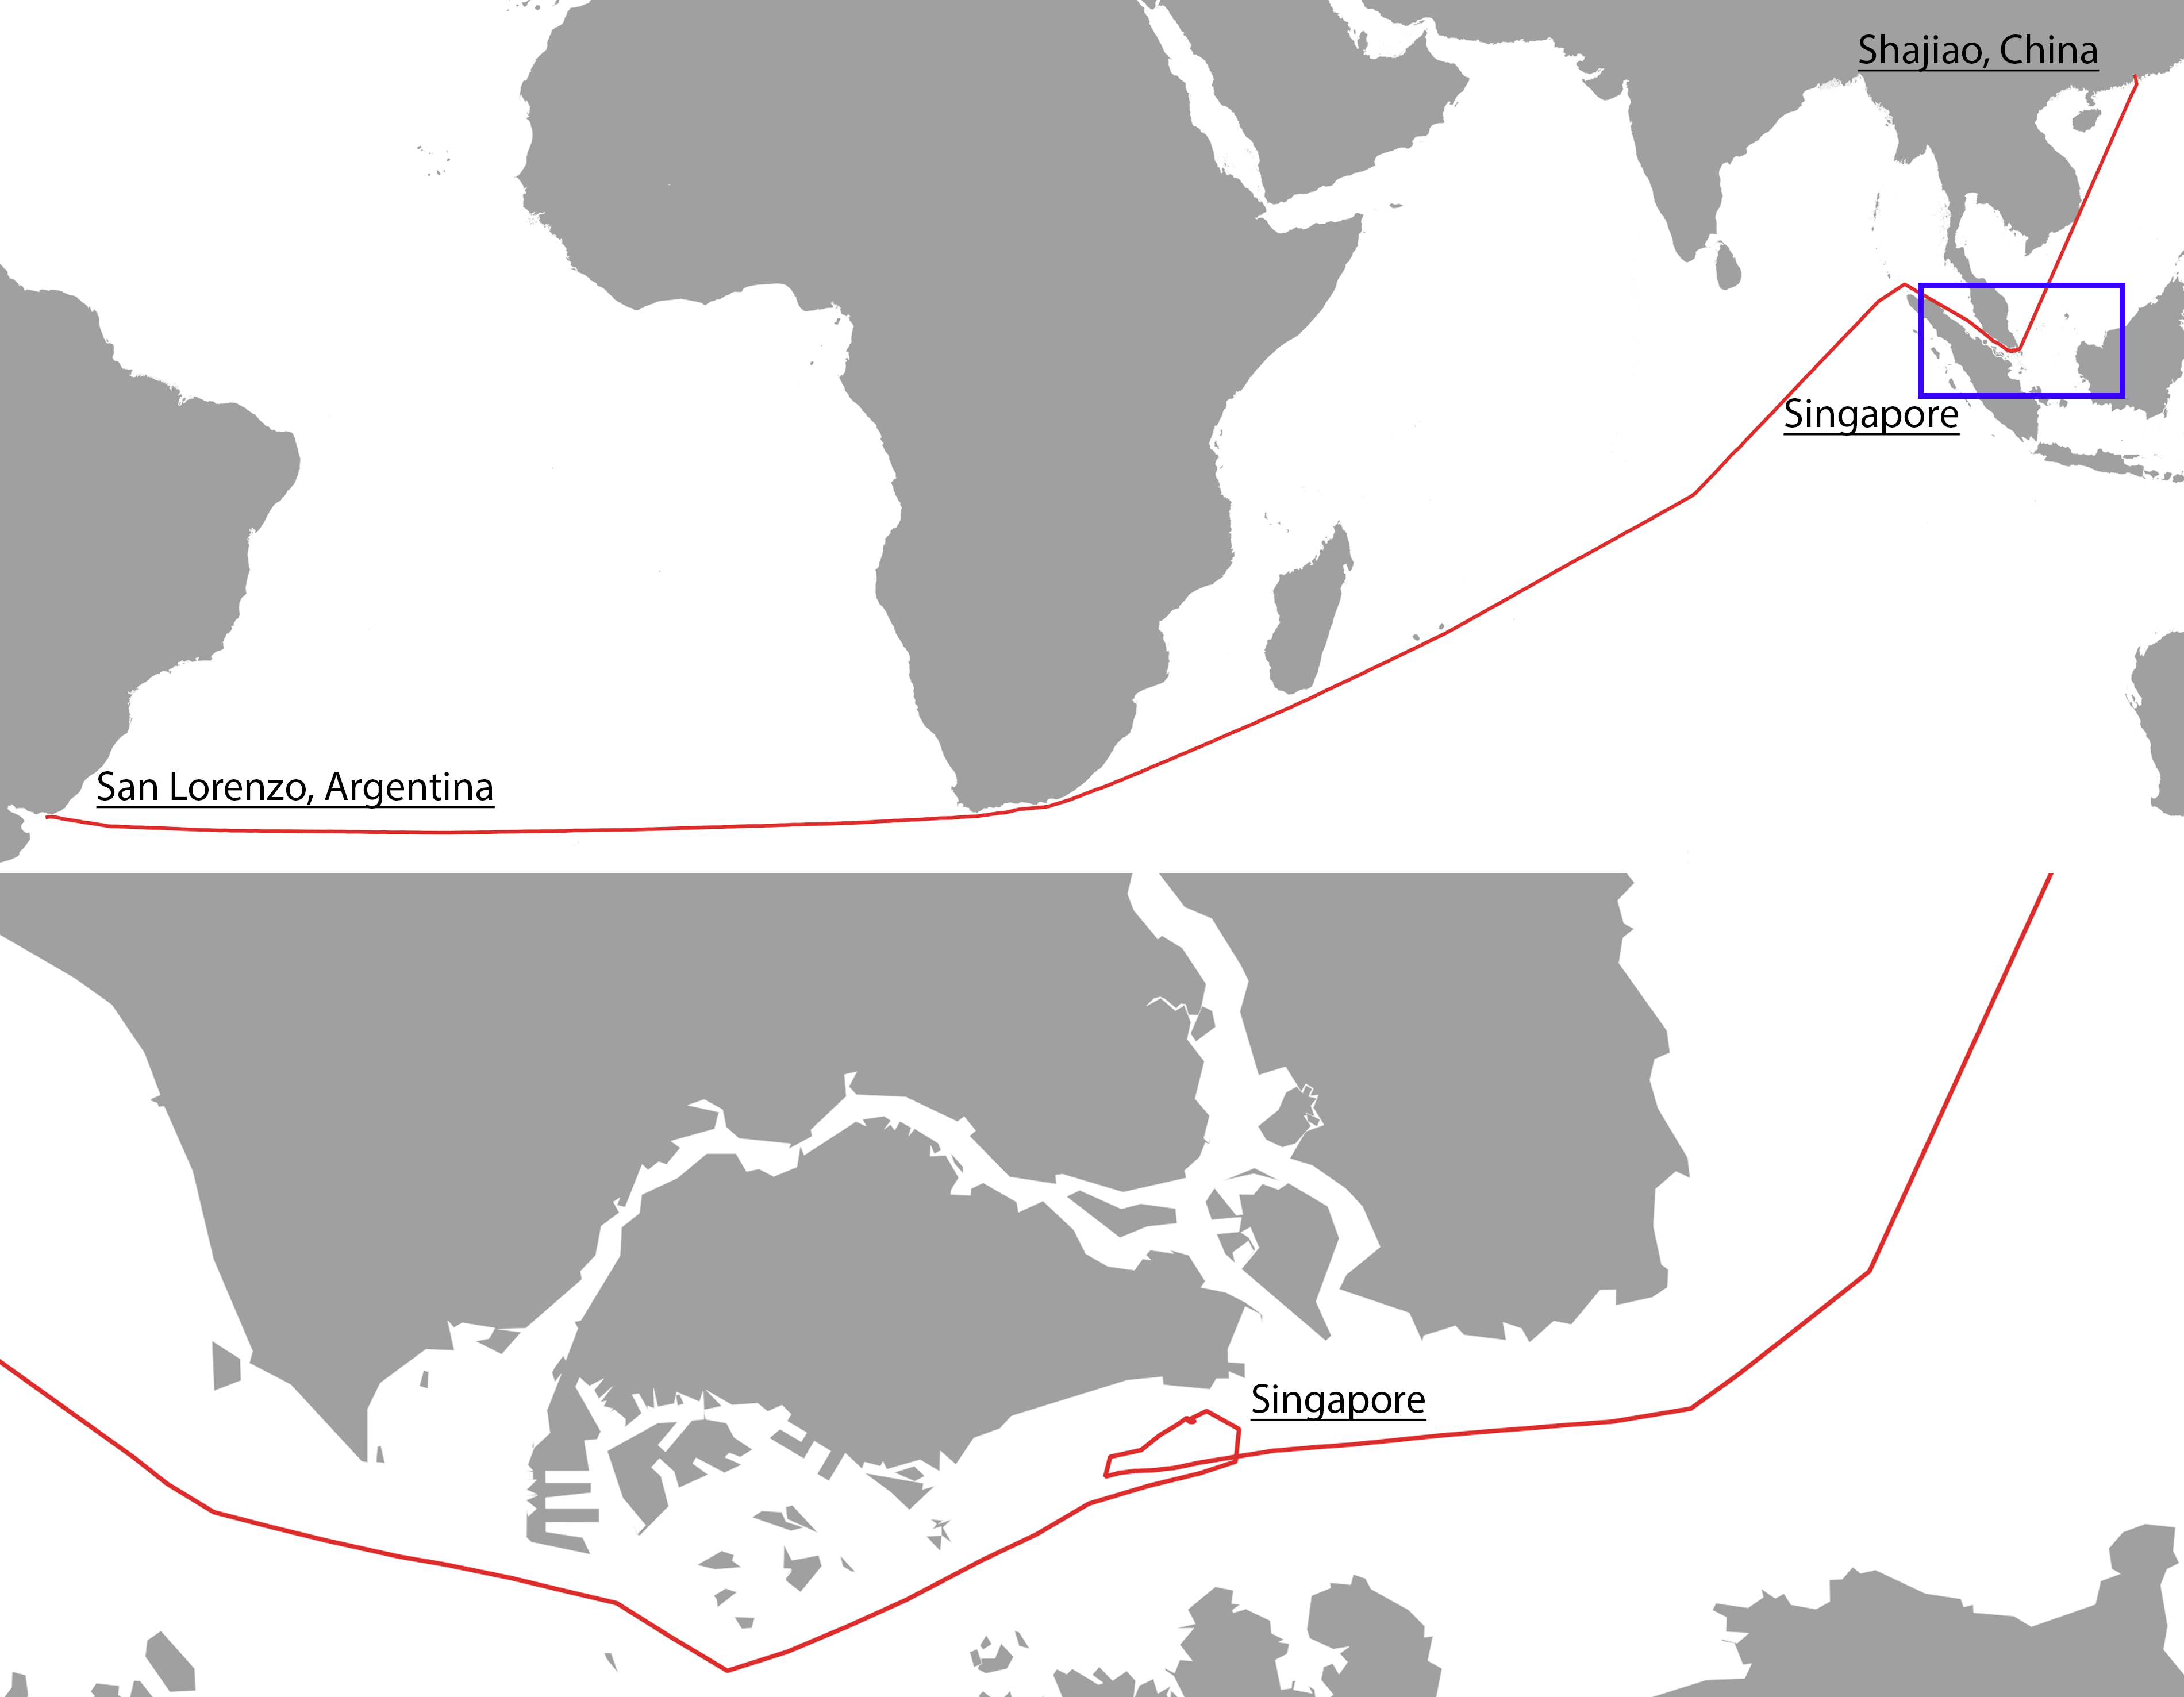
\includegraphics[width=1.0\textwidth]{figures/results/voyage_quality}
    \caption{Transition voyage from China to Argentina that visits the port of Singapore exemplifying the properties of the chosen voyage definition.}
    \label{fig:transition_voyage}
\end{figure}

The \textbf{1.7} million voyages constructed using the vessel transitions were sampled based on 6 hour intervals and collected in ``sampled\_transition\_voyages'' that formed the foundation for trajectory similarity measurements. In the process of constructing the final dataset, these sampled voyages were divided into multiple incomplete voyages up to a factor of four. The resulting training dataset collected in the table ``ml\_training\_data'' consisted of \textbf{4.3} million voyages.

\subsection{Trajectory similarity and MSTD}

Using the foundation of the sampled trajectories, each trajectory was compared to every other trajectory departing the same port to calculate the \acrfull{mstd}. The \acrshort{mstd} value was used primarily as a method of abstracting geographical trajectories into categorical and numerical values that a \acrfull{ml} model could work with. This process converted a voyage's geographical trajectory into MSTD, the similarity value to the most similar trajectory, and trajectory length. Thus, the MSTD value served as an initial prediction purely based on geographical trajectory similarity measurements using \acrfull{sspd}. The \acrshort{sspd} method was chosen for its ability to effectively handle different lengths and shapes of trajectories when estimating similarity. Furthermore, in the approach proposed in \cite{Zhang2020AISApproach} the \acrshort{sspd} method performed the best out of the algorithmic approaches evaluated, although, their own Random Forest (RF) based approach performed the best. However, the way the training data is structured, the trajectory similarity method of choice is completely interchangeable with others. The only requirement for a given trajectory similarity measurement is that it also produces a similarity value that serves as a weight for the \acrshort{mstd} value.

\acrshort{mstd} as an initial prediction seemed to be a decent initial indicator as to where the vessel would be arriving. In total, there were \textbf{4 306 271} entries in the final training data generated where exactly \textbf{1 423 476} of which has the same arrival port and \acrshort{mstd} value. Thus, it can be assumed that the purely spatial prediction using incomplete sampled historical voyages based on \acrshort{sspd} was \textit{33\%} accurate. In other words, when using an algorithmic prediction approach based on purely spatial trajectory similarity measurements, voyage destinations can be predicted correctly one third of the time. This formed a baseline accuracy to beat with the \acrshort{ml}-based solution.

\subsection{ML data preparation}

After the final training dataset was built, it was discovered that in terms of arrival port frequencies, the dataset was imbalanced thus making it harder for \acrshort{ml} models to learn. Although some models can better handle dataset imbalance, a sampling approach was used to balance the dataset before training to support different ML models. Several different sampling approaches were evaluated, however, the traditional over and under -sampling methods either produced massive amounts of synthetic data, or removed almost all the original data which was shown in \cref{fig:all_samplers} in \cref{chap:method}. Thus, an ensemble sampling method of majority undersampling and ``SMOTE+ENN'' was employed to balance the dataset before training. \cref{fig:ensemble_sampler} shows the results from the ensemble sampling method that uses a combination of under and over -sampling techniques. As \cref{fig:ensemble_sampler} shows, using a subset of the full dataset, the final result is 8\% smaller than the original dataset, is a lot more balanced, but still has differences in class frequencies which persisted from the original dataset.

\begin{figure}[htbp]
    \centering
    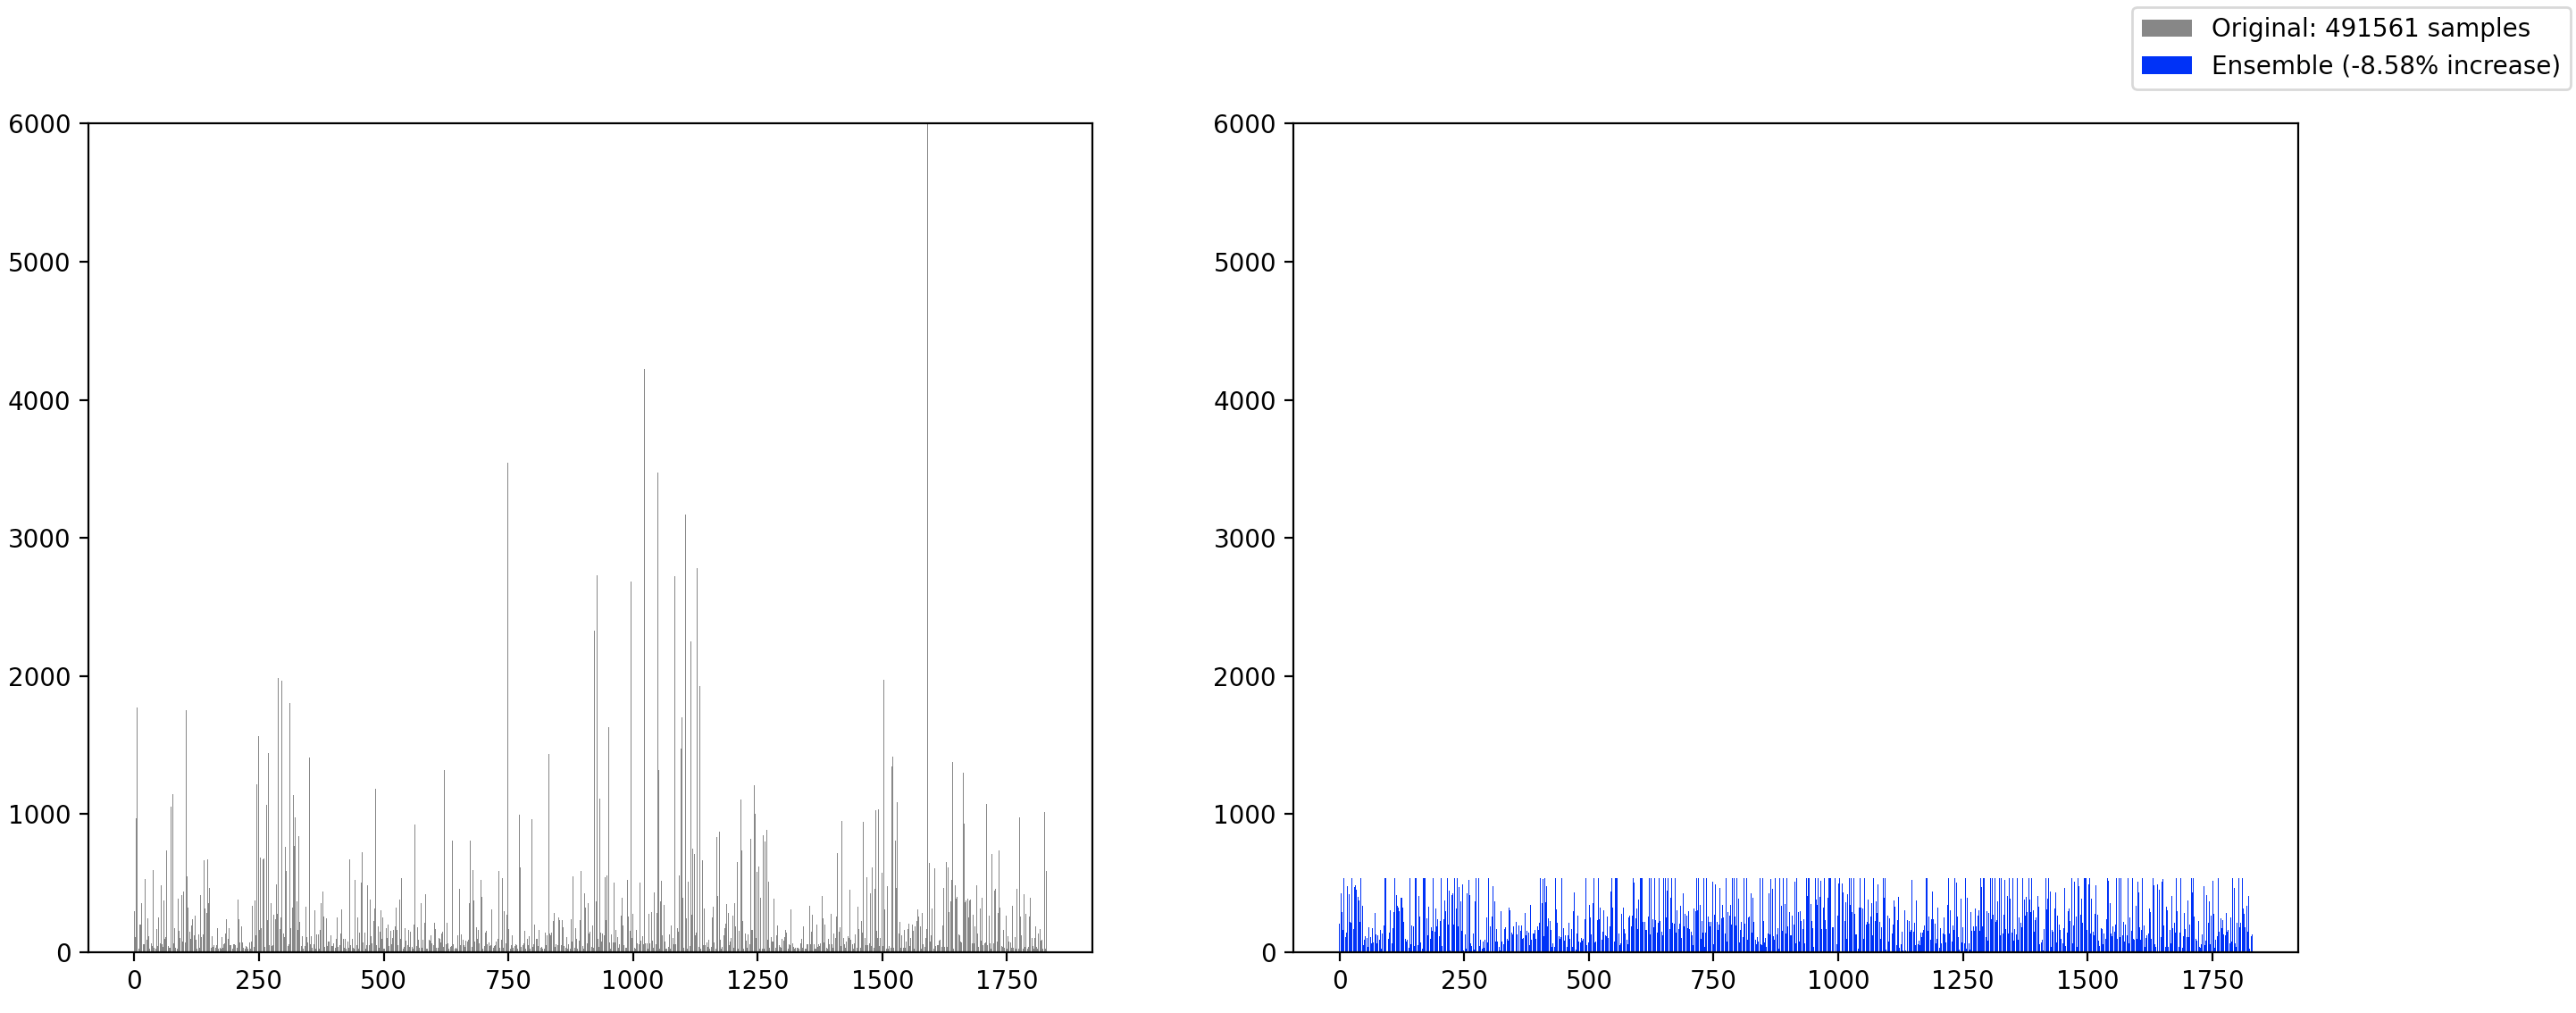
\includegraphics[width=1.0\textwidth]{figures/imbalance/ensemble}
    \caption{Final ensemble sampling method (right) compared to original dataset (left) where the final ensemble produces a dataset similar in size to that of the original.}
    \label{fig:ensemble_sampler}
\end{figure}

\section{Model training and prediction performance}

After the training dataset was constructed, encoded, and balanced, the model was trained using different approaches as described in \cref{sec:training_process}. This section describes the results from the training processes, the final approach used, and the resulting model's performance and predictions resulting from the evaluation process described in \cref{sec:evaluation_process}.

\subsection{Training process}

As described in \cref{sec:training_process}, multiple training processes were evaluated in order to find the most appropriate method of training a larger model on an extensive dataset. For the \acrfull{xgb} model, three different training processes were evaluated in this process.

First, the iterative approach was evaluated by training the model in batches of \textit{600 000} samples at the time. This approach seemed to work as intended, however, it was discovered that during subsequent training batches, the performance of the model dropped off for each iteration. It seemed as if the model did not handle continuous training of the same model as well as it does when training one model from scratch using the complete dataset. Furthermore, the parameter \textit{``early\_stopping\_rounds''} was used in the other approaches as a method of telling the model to stop training if it does not see any improvements after the given number of rounds. When this parameter is set using the iterative approach, the model can stop producing new trees before it has constructed the total number of trees allowed by the \textit{``n\_estimators''} parameter. Since the first iteration can produce a model with less trees than allowed, the next iteration fails as the number of allowed trees does not match with the previous model's actual number of trees. Although there are ways around this issue, as using the early stopping rounds parameter is useful to avoid overfitting, the iterative approach did not seem the most appropriate during the development process.

Next, it was attempted to train the model using the external memory, or ``out-of-core'' memory version of \acrshort{xgb}. In this approach, the \acrshort{xgb} library is provided a \textit{libsvm} file which it converts to an optimized matrix format which is kept on the computers file system. However, all attempts at training the model using external memory were unsuccessful as the training process consumed all of the running computer's available memory and resulted in a ``bad allocation`` memory error. There seems to either be a misconfiguration or an underlying issue with the Python library used in the implementation. However, since the expected results from this approach should be the same as training the model in one iteration on a capable computer, these issues were not further looked into, although, it could be beneficial to reduce the resource requirements for the training process for future use. Therefore, it could warrant more investigation for future work.

Finally, the entire dataset was used to train the final model in one iteration on a computer capable of running the process. The training process ran over the course of two days and consistently required around 200GB of memory. The vast memory consumption could be somewhat reduced by not evaluating the model during the training process which is appropriate for future training processes after the model has been trained and the training configuration has been validated. As described in \cref{sec:training_process}, an extra copy of the training and test datasets were kept in memory to continuously evaluate and monitor the training process.

\subsection{Performance}

During the training process, the performance of the model was continuously evaluated to measure logarithmic loss and multi-class classification error. \cref{fig:eval_set} shows these metrics plotted over each boosting round in the training process. Both graphs starts converging at 100 decision trees have been constructed at around \textbf{1.5} log loss, and around \textbf{0.3} classification error. This corresponds to around \textbf{70\%} accuracy. Since the graphs have not completely converged, it is possible to either increase the learning rate parameter or increase the number of estimators in the tree, although it seems as if the graphs are very close to converging, so it might not increase performance noticeably and increases risk of overfitting. As there is very little difference between the performance on the training set and evaluation set, it indicates that the model is not overfitting, however, it might indicate that the model is over optimistic. This could occur when there are several similar samples in the training and the test datasets and could be a consequence of the sampling techniques used to balance the dataset.

\begin{figure}[htbp]
    \centering
    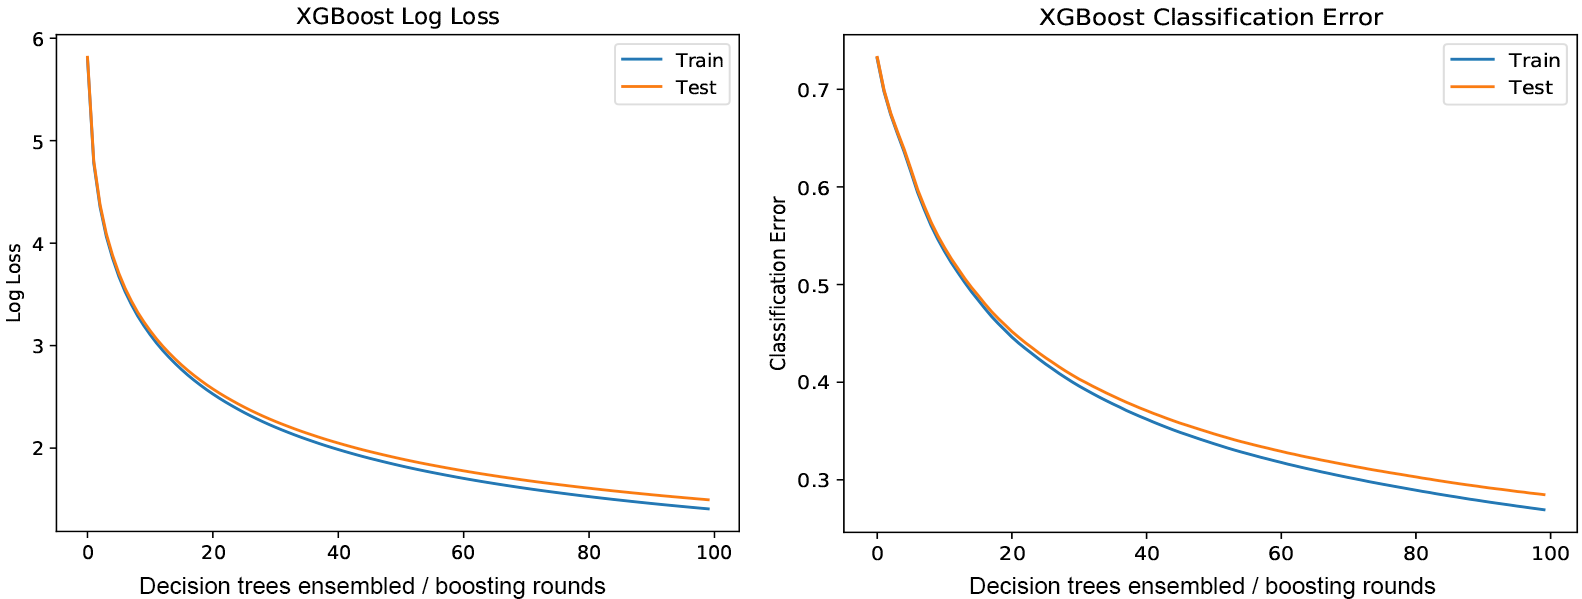
\includegraphics[width=1.0\textwidth]{figures/results/eval_set}
    \caption{Logarithmic loss and classification error metrics tracked per boosting round in the training process.}
    \label{fig:eval_set}
\end{figure}

After the training process finished, the test dataset was used to make predictions to further evaluate the results. From the resulting predictions, accuracy was calculated to be \textbf{72\%}, and a class report was generated that shows more metrics for each possible class, or encoded arrival port, that might provide more insight into the model's performance than accuracy. \cref{lst:class_report} shows a summarized output from this class report showing the metrics precision, recall, f1-score, and support for each class as well as the aggregated mean values from all of the classes. As mentioned in \cref{sec:model_evaluation}, f1-score is based on precision and recall and is particularly appropriate for measuring performance on imbalanced datasets, and as \cref{lst:class_report} shows, the f1-score does not deviate much from the estimated accuracy of \textbf{72\%}, or \textbf{0.72}. This indicates that the accuracy value is reliable and is not biased by dataset imbalance.

\begin{lstlisting}[
    caption={Class report based on prediction results from the test dataset. The performance of the classifier is evaluated per class by using precition, recall, f1-score, and support.},
    label=lst:class_report,
    showstringspaces=false,
    basicstyle=\ttfamily,
]
[XGBoostClassifier] Class Report:
             precision    recall  f1-score   support      pred
0             0.378049  0.240310  0.293839     258.0     164.0
1             0.816850  0.810909  0.813869     275.0     273.0
2             0.722222  0.541667  0.619048     312.0     234.0
3             0.672727  0.377551  0.483660     294.0     165.0
...           ...       ...       ...          ...       ...
3067          0.824675  0.849498  0.836903     299.0     308.0
3068          0.833922  0.778878  0.805461     303.0     283.0
3069          0.773050  0.762238  0.767606     286.0     282.0
3070          0.614035  0.557325  0.584307     314.0     285.0
...           ...       ...       ...          ...       ...
avg / total   0.718698  0.715150  0.712737  878049.0  878049.0

\end{lstlisting}

Lastly, in order to ensure the model is not overfitted, a three-fold cross validation process was employed. \cref{lst:cv_result} shows the results from the three folds that the model was trained on. It is recommended, or common to use more folds ranging from five to 10, however, because of the long training time and time limitations, only three folds were used. As described in \cref{sec:model_evaluation}, since the standard deviation (noted as ``std. dev.'' in \cref{lst:cv_result}) is low, the model is likely to not be overfitted.

\begin{lstlisting}[
    caption={Output from 3-fold cross validation. \todo{update numbers}},
    label=lst:cv_result,
    showstringspaces=false,
    basicstyle=\ttfamily,
]
 Folds:      [0.70569399 0.71297481 0.72244745]
 Mean:       0.7137054183485277
 Std. dev.:  0.006859056778768982
\end{lstlisting}

\section{Prediction results}

After the model was trained and evaluated, \textit{20\%} of the total training dataset was used to evaluate the model. This evaluation process resulted in around \textit{880 000} example predictions. These predictions were further analyzed to discuss the impact and meaning of the different features used in the dataset. These results are presented in this section.

\subsection{Feature importances}

An added benefit of using a tree based model such as the \acrfull{xgb} or \acrfull{rf} model is that they can provide insight into the importances of features, or attributes. In a decision tree based ensemble, when constructing a tree, the training data is analyzed to find the best features to make splits, or branches, in the trees. After the training process, the models can then produce a ranking over what features best divided the dataset best. This is referred to as feature importance.

\begin{table}[htbp]
    \centering
    \begin{tabularx}{0.6\textwidth}{X X}
        \bfseries{Feature} & \bfseries{Importance} \\ \toprule
        sspd\_mstd         & 0.443659 \\ \midrule
        departure\_port    & 0.226288 \\ \midrule
        segmentation       & 0.180907 \\ \midrule
        sspd\_dist         & 0.083816 \\ \midrule
        trajectory\_length & 0.065331 \\ \bottomrule
    \end{tabularx}
    \caption{Feature importances based on the \acrshort{xgb} decision tree ensemble process}\label{tab:feature_importances}
\end{table}

\cref{tab:feature_importances} shows an overview of the produced feature importances after the \acrshort{xgb} training process. As it shows, the most important feature was the \acrshort{mstd} value at a ranking of 0.44 out of 1.0, followed by the vessel's departure port, segmentation value, and then the similarity value and voyage length. This analysis can further help decide if features are worth dropping from the dataset, and insight into what attributes are good indicators during voyage predictions. As mentioned in \cref{sec:dataset_imbalance}, the attributes ``segment'', and ``sub-segment'' were combined into one segmentation value in order to ensure that no invalid segment and sub-segment combinations could be generated by sampling methods. A disadvantage of this is that the feature importances of the two attributes are lost in favor of the combined value. However, from test runs made during the development process with and without sampling, the importance of segment and sub-segment were usually ranked where segmentation is in \cref{tab:feature_importances} with sub-segment being more important than segment.

Furthermore, the results from test dataset predictions were analyzed to find the impact of the attributes that mostly served as weights for the \acrshort{mstd} value, namely, the similarity value (\textit{sspd\_dist}) and trajectory length. \cref{lst:dist_length_impact} shows an output from the evaluation process which shows that the distance value was smaller, on average, for correct predictions while trajectory length did not considerably differ from correct and incorrect predictions. It makes sense that the distance, or similarity, value is lower for correct predictions as the more similar the most similar historical trajectory is, the more valuable the \acrshort{mstd} value is. For instance, if a voyage's most similar historical trajectory has a \textit{sspd\_dist} of 0, it is following an exact path of a previous voyage. In this case, the similarity value for correct predictions was on average around \textit{43\%} lower than for incorrect predictions. For the trajectory length, it would make sense that the longer the voyage had traveled, the easier it would be to predict its destination, thus, the length should be longer for correct predictions. However, this is not the case for these predictions. This could be explained by the fact that shorter voyages might be easier to predict than long voyages for small vessels. For instance, it is presumable that, passenger vessels with very short but frequent trajectories are very easy to predict thus bringing the average length down for correct predictions. To confirm this hypothesis, further investigation into the specific segments and sub-segments is required.

\begin{lstlisting}[
    caption={Mean values of similarity value and trajectory length for correct and incorrect predictions.},
    label=lst:dist_length_impact,
    showstringspaces=false,
    tabsize=1,
    basicstyle=\ttfamily,
]
mean ssp_dist for correct predictions:           115642.48170757179
mean trajectory_length for correct predictions:  17.662729492637958

mean ssp_dist for erroneus predictions:           201713.174255885
mean trajectory_length for erroneus predictions:  18.841843522761508
\end{lstlisting}

\subsection{Segment predictability}

As it relates to research question 2 (\cref{sec:research_questions}), the \textit{880 000} predictions from the test dataset were further analyzed in search of patterns in predictability of different types of vessels. These results also serves to gain further insight into the value of the performance metrics. \cref{fig:segment_accuracy} shows a bar chart of the initial accuracy of predictions per segment, and it shows that there are some differences in accuracy per segment overall, but the most of the segments have a similar level of predictability. For example, vessels of the segment ``other'' were the easiest to predict and had the highest accuracy of \textit{76\%}. This is likely to be caused by different types of passenger vessels that lie within this segment. These vessels produce many predictable voyages as they travel between a few number of ports with a high frequency. Furthermore, the ``other'' segment also include very specialized vessels that are limited in terms of possible destination ports.

\begin{figure}[htbp]
    \centering
    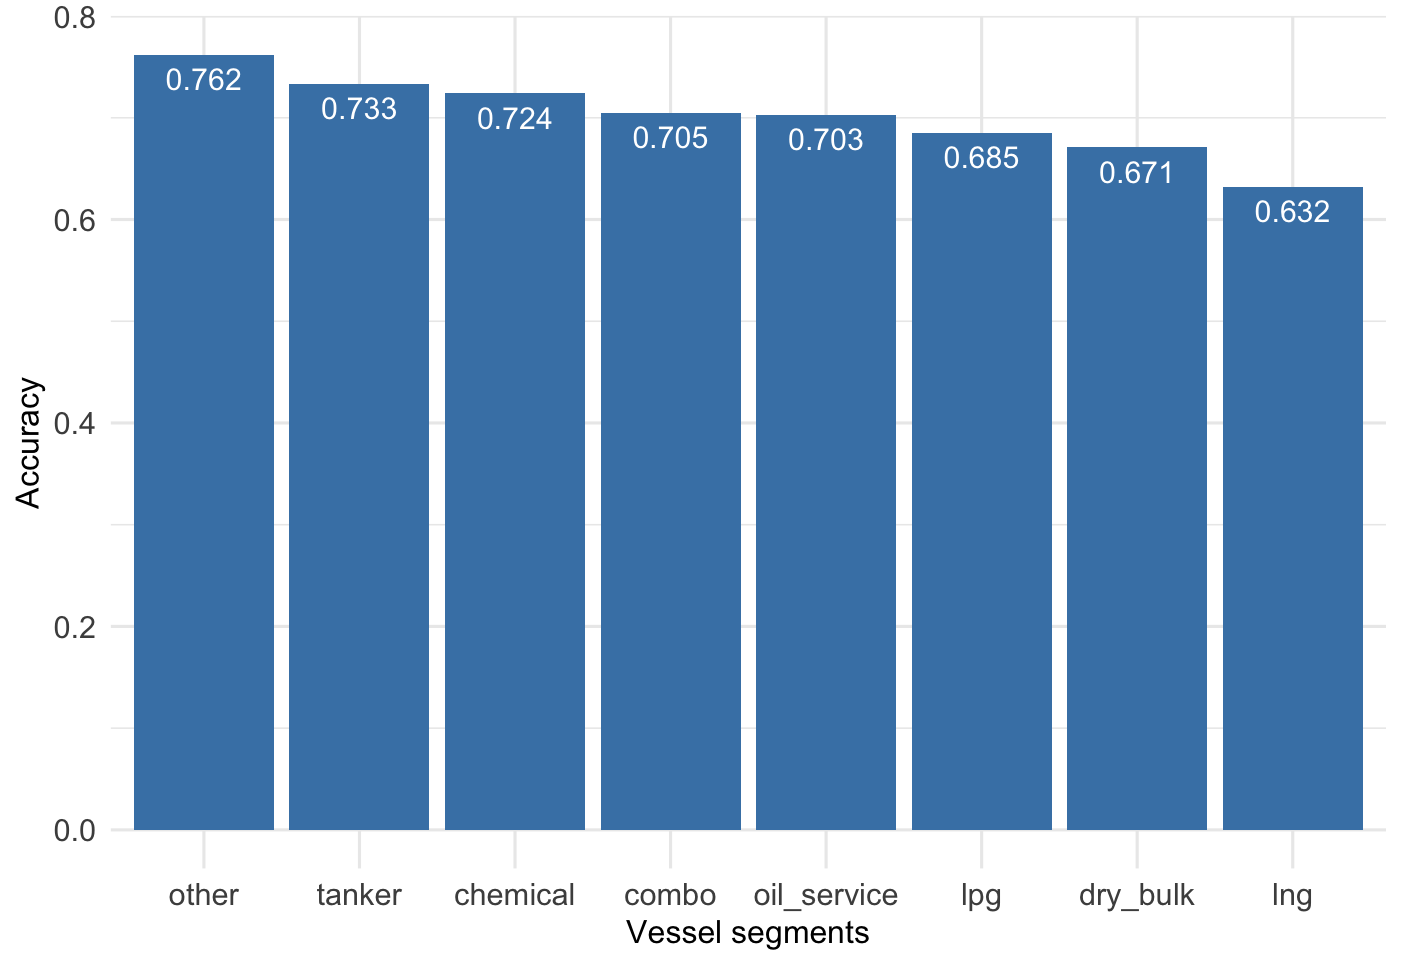
\includegraphics[width=0.8\textwidth]{figures/results/segment_accuracy_new}
    \caption{Accuracy of predictions from test set per segment.}
    \label{fig:segment_accuracy}
\end{figure}

As \cref{fig:other_accuracy} shows, and as expected, the accuracy of the passenger related sub-segments were very high. Since these are so high in frequency and has shorter trajectories, they may be the main cause that the average trajectory length was lower for correct predictions than incorrect ones. On the other hand, container and car ``roll on/roll off'' (roro) vessels travel longer distances less frequently but were also quite predictable. Another segment that could affect the average trajectory length and similarity values for correct predictions is the oil service segment. The oil service vessels should be easy to predict as these vessels travel to oil platforms and often back to the same or another nearby port. However, for these vessels, their trajectories would have been harder to consider as they often do not use the ``moored'' AIS navigational status when arriving at oil platforms. This can lead to very long trajectories that are hard to compare to others, therefore, these vessels should rely more on the departure port rather than the \acrshort{mstd} related values. In general, the ``other'' and ``oil service'' segments are not very relevant for \acrfull{mo}'s customers or for bigger actors in the industry, however, some sub-segments such as container and other general cargo ships can be quite relevant.

\begin{figure}[htbp]
    \centering
    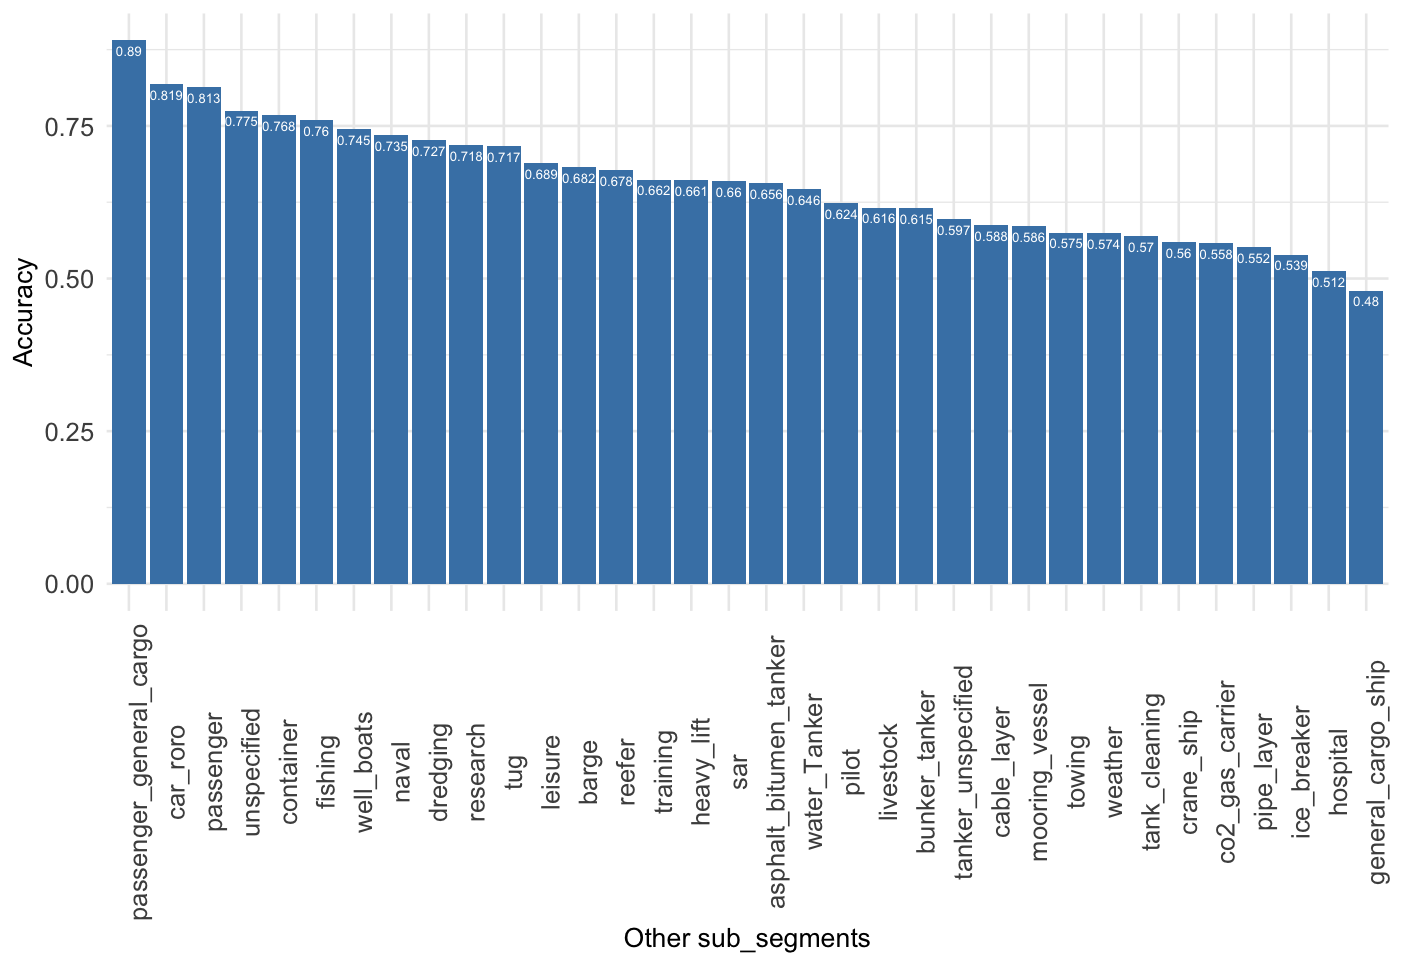
\includegraphics[width=1.0\textwidth]{figures/results/seg_other_acc}
    \caption{Accuracy of predictions per sub-segment within the ``other'' segment.}
    \label{fig:other_accuracy}
\end{figure}
\begin{figure}[htbp]
    \centering
    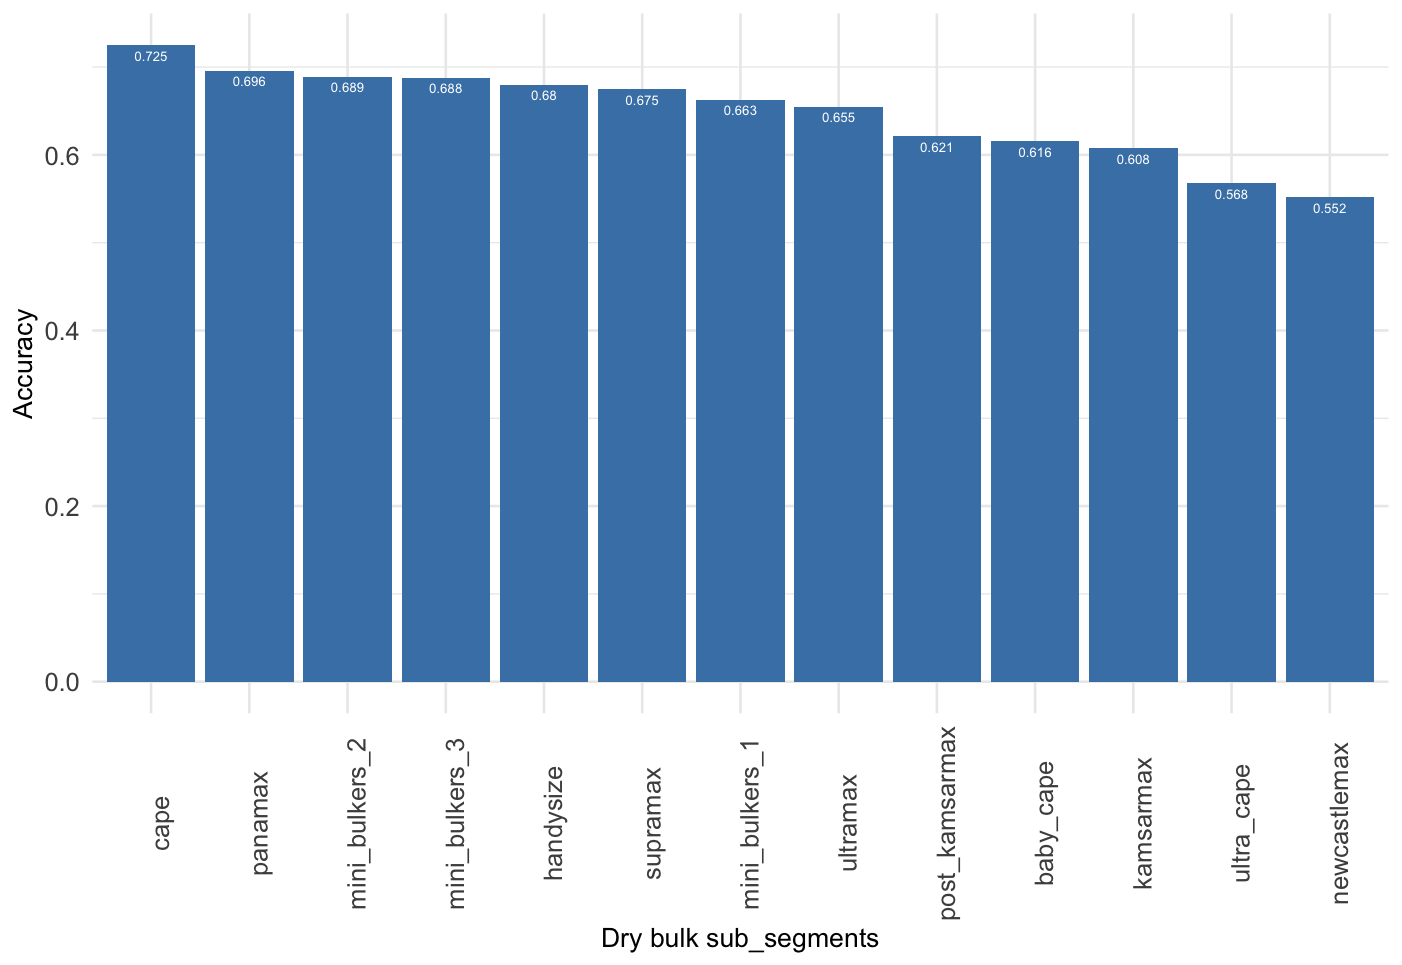
\includegraphics[width=0.8\textwidth]{figures/results/seg_dry_bulk_acc}
    \caption{Accuracy of predictions per sub-segment within the ``dry\_bulk'' segment.}
    \label{fig:dry_bulk_accuracy}
\end{figure}


The dry bulk cargo industry, on the other hand, has more commercial interest. \cref{fig:dry_bulk_accuracy} shows the accuracy per sub-segment for the dry bulk cargo segment. The dry bulk sub-segments are based on the vessels' cargo capacities and sizes, however, as \cref{fig:dry_bulk_accuracy} shows, there seems to be little correlation between vessel size and accuracy. The two most accurately predicted sub-segments are large vessels, however, they are followed closely by the smaller sub-segments, and the two least predictable types are some of the largest. Thus, the uniqueness of the sub-segment value itself had more impact on predictions than the implied size and capacity of the vessels.

\begin{figure}[htbp]
    \centering
    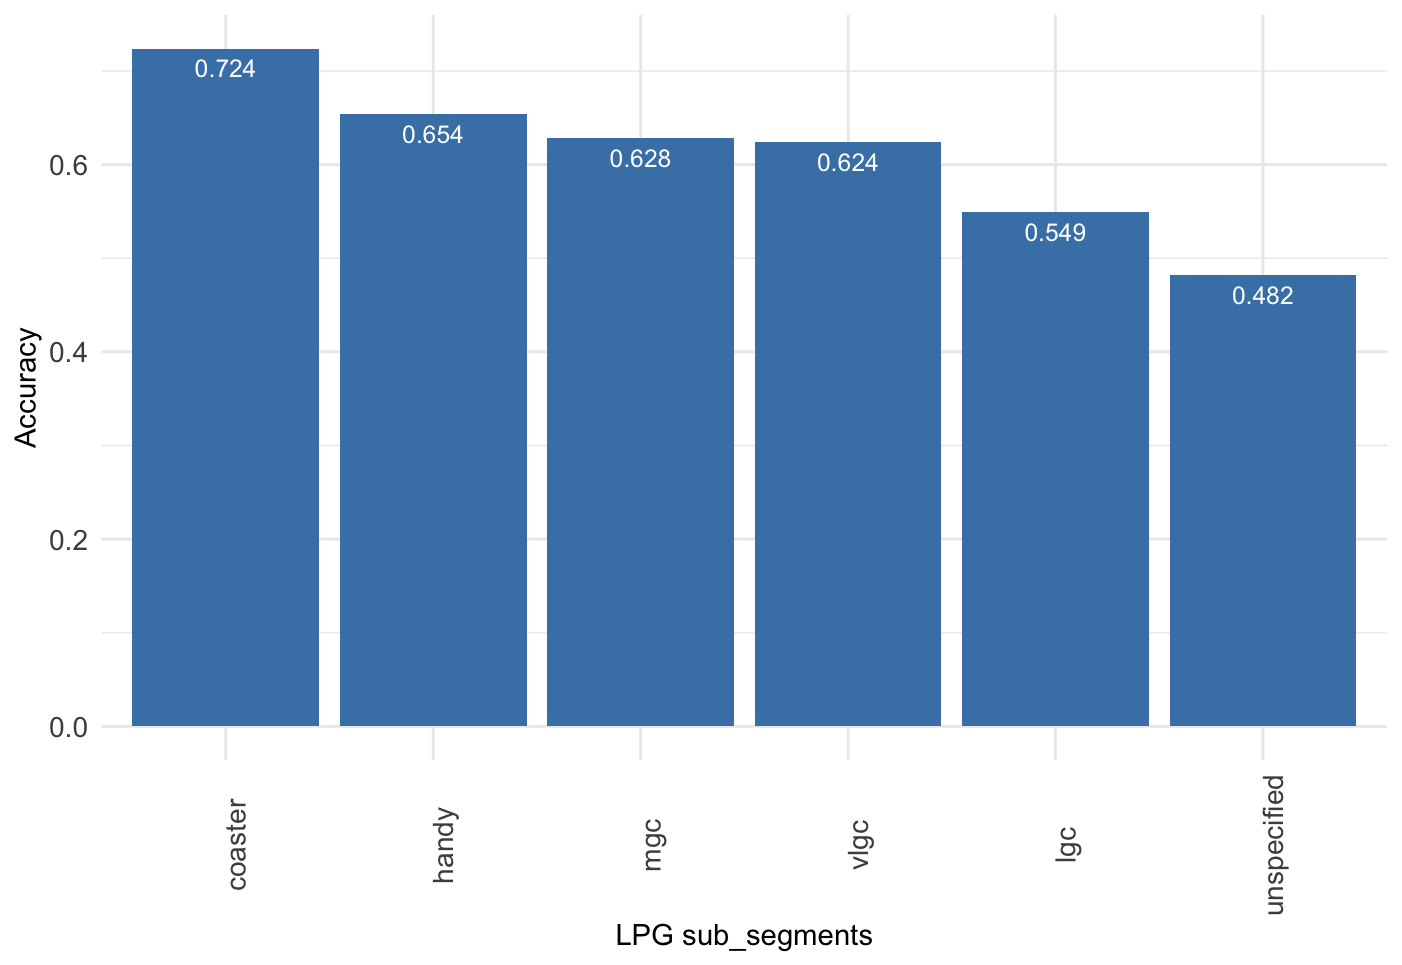
\includegraphics[width=0.9\textwidth]{figures/results/seg_lpg_acc}
    \caption{Accuracy of predictions per sub-segment within the ``LPG'' segment.}
    \label{fig:lpg_accuracy}
\end{figure}

The prediction results for tanker sub-segments show similar results as to the dry bulk ones, however, some other segments does seem to show that size and capacity indeed might be correlated to predictability in different ways. For instance, in the chemical segment the two largest sub-segments have the highest accuracies of \textit{90\%} and \textit{85\%}, however, the remaining sub-segments does not show much difference correlated to size. There seem to be a slight correlation in chemical vessels that show that larger vessels are easier to predict than smaller ones, however, for other segments the opposite correlation seems to occur. The \acrfull{lng} and \acrfull{lpg} vessels have the highest correlation between size and accuracy, but in the opposite direction compared to the chemical vessels. \cref{fig:lpg_accuracy} shows that the three smallest \acrshort{lpg} sub-segments \textit{coaster}, \textit{handy}, and \textit{MGC} have the highest accuracy, while the two largest sub-segments \textit{VLGC} and \textit{LGC}  have lower accuracies. This is similar to that of the \acrshort{lng} vessels (\cref{fig:lng_accuracy}) where the largest sub-segments \textit{QMax}, and \textit{QFlex} are harder to predict than the smaller sub-segments.

\begin{figure}[htbp]
    \centering
    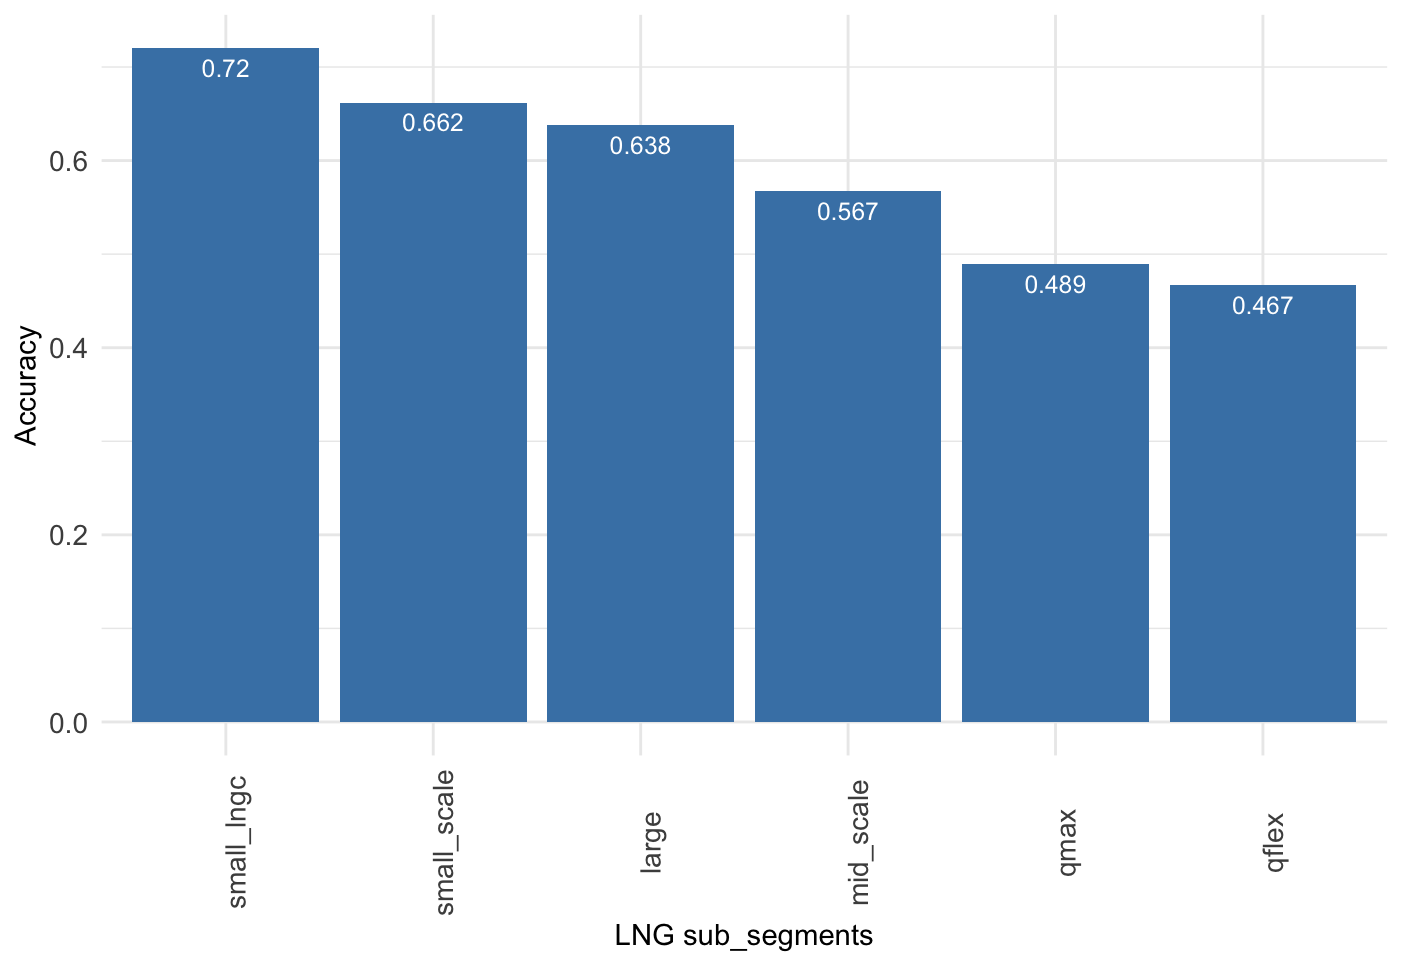
\includegraphics[width=0.9\textwidth]{figures/results/seg_lng_acc}
    \caption{Accuracy of predictions per sub-segment within the ``LNG'' segment.}
    \label{fig:lng_accuracy}
\end{figure}

Another interesting segment to analyze is the combo segment. These combination vessels can serve multiple functions in that they can carry different types of cargoes. In \cref{fig:segment_accuracy}, the combo segment showed a mid-range general accuracy level, however, when looking into the sub-segments, there are substantial differences in accuracies across the different types of combo vessels (\cref{fig:combo_accuracy}). The ``Klaveness Combination Carriers'' (CABU) and ``Oil-Bulk-Ore'' (OBO) vessels have the highest accuracies. However, there are only 12 CABU vessels and 5 OBO vessels in the world, or in \acrfull{mo}'s vessel database. On the other hand, there are 4700 chemical product tankers in the world that were also quite predictable. These vessels drive the general accuracy of the combo vessels up in \cref{fig:segment_accuracy} as the remaining sub-segments have substantially lower accuracies. It does, however, make sense that combo vessels are generally difficult to predict as they serve multiple functions which results in them having more possible destination ports they can load and unload at.

\begin{figure}[htbp]
    \centering
    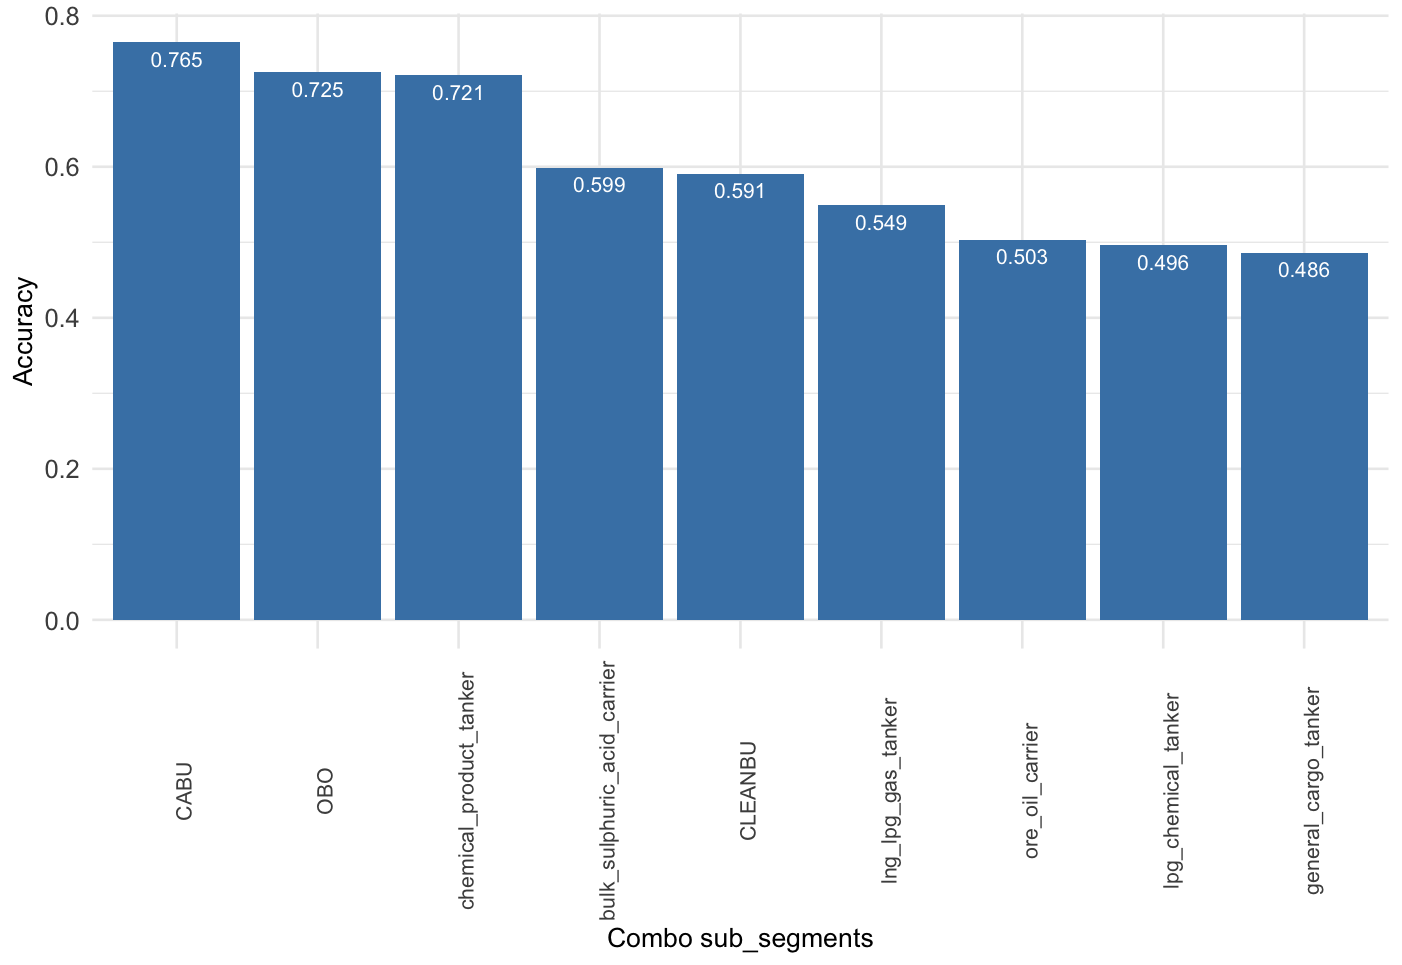
\includegraphics[width=0.9\textwidth]{figures/results/seg_combo_acc}
    \caption{Accuracy of predictions per sub-segment within the ``combo'' segment.}
    \label{fig:combo_accuracy}
\end{figure}

In regards to \texttt{RQ2} (\cref{sec:research_questions}), vessel segments and sub-segments seem to have a substantial impact on the predictability of vessels. As shown in \cref{tab:feature_importances}, the vessel segmentation had a feature importance close to that of the vessel's departure port. Furthermore, as discussed throughout this section, there are differences in accuracies for different segments and sub-segments, therefore, the vessel segmentation, with sub-segments in particular, had a significant impact on the predictions in the test dataset used during the evaluation process.

In regards to \texttt{RQ2a} the most predictable segment overall was the ``other'' segment (\cref{fig:segment_accuracy}). This was not entirely surprising as the sub-segments including passenger vessels are very predictable (\cref{fig:other_accuracy}). Moreover, the tanker, chemical, and combo vessels were similar in their accuracy levels, while \acrshort{lpg}, dry bulk, and \acrshort{lng} vessels were slightly less predictable. The sub-segment ``chemical product tanker'' drove the accuracy of the combo segment up to a similar level to that of the tanker and chemical vessels. This can be explained by the fact the this specific sub-segment has overlap into the two other segments. In other words, several tanker and chemical vessels are also present in the ``chemical product tanker'' combo sub-segment, so the accuracies is expected to be similar between the specific sub-segment and the tanker and chemical segments.

In response to \texttt{RQ2b}, and as mentioned earlier in this section, there seems to be some correlation between vessel size, capacity, and predictability, however, this only seems to be the case for some segments while for others, the uniqueness of the sub-segment value was the more important factor than the implied size or capacity. Thus, in regards to \texttt{RQ2b}, the prediction results does not conclusively indicate that larger vessels are more predictable than others.


\section{Applications and validity}

After the final training process, the resulting model is capable of predicting the future destination ports of traveling vessels. This section describes the intended usage and applications of the developed model as well as validation from experts in the industry.

\subsection{Usability}

As summarized in \cref{sec:pred_summary}, the process of predicting a single vessel's future destination port consists of first collecting the current traveling trajectory by fetching the positional \acrshort{ais} records from the last detected ``moored'' navigational status was transmitted to the last transmitted position. This trajectory must then be simplified as described in \cref{sec:trajectory_sampling}, then the \acrfull{mstd} of the must be calculated using the \acrshort{sspd} method with the traveling trajectory and every other historical trajectory departing the same port. The vessel's \acrshort{mstd}, segmentation, the distance returned from the \acrshort{sspd} method, and the length of the trajectory can be used to predict the vessel's next destination. The final trained model is saved to a file so it can quickly be loaded when making predictions. Thus, a program can be written that reads the trained model, receives an outgoing voyage, and predicts its next destination port.

In regards to re-training the model with new data, two approaches can be used. The simplest but more time consuming approach is to completely retrain the model after a substantial amount of new data is available. The training process takes around two days to complete using all of the historical dataset using a capable computer. Another approach could be to use \acrfull{xgb}'s support for iterative, or continuous learning as described in \cref{sec:training_process}. After the training process has completed, the \acrshort{xgb} model can be saved to file for future evaluation and predictions.

\subsection{Expert validation}

\begin{itemize}
    \item Caveats/use-cases and value
    \item Evaluation from MO
    \item Evaluation from external actors
\end{itemize}

\chapter{Discussion}

\section{Summary}

\begin{itemize}
    \item Brief summary of the entire process
\end{itemize}

\section{Dataset and problem formulation}

\subsection{Vessel voyage definition}

\subsection{Geographical trajectory abstraction and MSTD}
\begin{itemize}
    \item Is MSTD an appropriate abstraction of trajectories.
    \item Are there other ways to combine trajectory predictions with additional voyage and vessel data?
    \begin{itemize}
        \item MSTD with more filters?
        \item Different trajectory similarity measurements?
        \item ML-based trajectory similarity normalized with port frequency considering segments?
    \end{itemize}
\end{itemize}

\subsection{Data preparation and dataset imbalance}
\begin{itemize}
    \item How was encoding appropriate?
    \item Was sampling appropriate, how did it affect results?
    \item Are there different sampling methods that could have been more appropriate?
\end{itemize}

\subsection{Data storage and architecture}
\begin{itemize}
    \item Scalability, availability. PostGreSQL DB structure advantages/disadvantages
\end{itemize}

\section{ML-based destination prediction}
\begin{itemize}
    \item Why did we get the described performance.
    \item Weaknesses/limitations
    \item Dataset vs real life
\end{itemize}

\section{Research questions and hypothesis}

\begin{itemize}
    \item How did I answer the research questions?
    \item Any additional hypothesis?
    \item How was what I did different from related works?
\end{itemize}

\subsection{Feature importances}

\subsection{Segment predictability}

\begin{itemize}
    \item Why are some segments easier to predict
    \item Why are some sub-segments easier to predict
\end{itemize}

\section{Real-life applications}

\begin{itemize}
    \item What is the value of this solution
    \item What can it be used for
    \item Response from external actors
    \item Is this something that contributes to the industry as well as academia
    \item Value for MO\@. Future applications and integrations in MO's product (teasers)
\end{itemize}

\section{Limitations and future work}

\begin{itemize}
    \item Voyage definition - anchoring, bunkering
\begin{itemize}
    \item AIS navigational status is manual input, can we better claim that a vessel has arrived/departed a port?
    \item clustering vs. transitions
\end{itemize}
    \item MSTD - trajectory similarity measurement. Zhang et al. achieved better results using RF than SSPD.
    \item Improving the model by adding more features such as weather, seasons, ballast/laden, \ldots more?
    \item Implementing at large scale providing on-demand predictions and availability
\begin{itemize}
    \item Implement a real-time updated voyage database
    \item Fetch every vessels current trajectory and estimate MSTD
    \item Pass all vessel data to ML model which, very quickly, predicts destination ports.
    \item Use a routing concept to get ETA (mesh-based routing, ais-based routing)
\end{itemize}
\end{itemize}

\subsection{Vessel availability}
\begin{itemize}
    \item Further implementation with MO's infrastructure.
    \item Give me all vessels that will be in port A at X time.
\end{itemize}


\chapter*{\bibname}
\printbibliography[heading=none]

% First paper

\begin{paper}{papers/landes1951scrutiny.pdf}{paper:scrutiny}
    Here, you may add a description of the paper, an illustration, or just give the bibliographic reference:
    \begin{quote}
        hello world
    \end{quote}
    Or you may leave it empty, if you like.
\end{paper}

% Second paper etc.

\appendix
\chapter{Feasibility study - Summary}

As already mentioned, the main motivation behind the thesis is derived from the observation that the existing methods of vessel destination prediction neglect data depth in their models. Especially, not considering the type and dimensions of vessels is presumed to be a major limitation of the existing literature. In order to establish this in an empirical manner, a feasibility study was conducted on the aspect of \acrfull{mo}'s novel segmentation of vessels. As part of the course work for the prior \acrshort{ntnu} course called \textit{“IMT4894 Advanced Project Work”}, such a feasibility study was  conducted to estimate the impact of vessel segmentation on the aspect of port frequencies. Port frequencies, or patterns of port arrivals and departures should reflect the fact that different vessels of different types travel in different patterns. Thus, if it is possible to show that segmentations have a significant impact on these patterns through port frequencies, it can be concluded that it will have an impact on vessel destination predictions.

The dataset used in this feasibility study mainly consisted of vessel transitions, and port data. The dataset also includes the vessel's segment and sub-segment. For a given port, every visiting vessel was assigned the attribute \textit{NextPort} that indicated the next arrival port after departing the given port. \cref{fig:apw_dataset} shows an example of vessels arriving at the port of Oslo (\texttt{NOOSL}).

\begin{figure}[htbp]
    \centering
    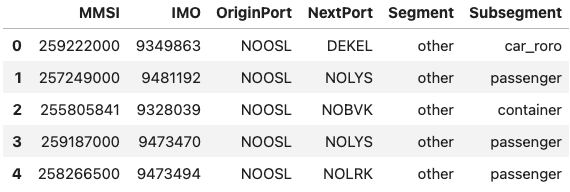
\includegraphics[width=.8\textwidth]{figures/apw/apw_dataset.png}
    \caption{A sample of the dataset used in the feasibility study}
    \label{fig:apw_dataset}
\end{figure}

In the feasibility study, there were two main steps in the analysis process. Firstly, a single-case analysis was conducted on a port known to the author to establish a more thorough overview of the traveling patterns of different vessel types and to gain an understanding of how to interpret the results. Secondly, a trend analysis was conducted on a collection of ports in order to establish a recurring pattern. In the study, a few major ports were selected combined with a few ports known to the author and experts in \acrshort{mo}. The complete list of ports are listed in \cref{sec:trend_analysis}.

\section{Single-case analysis}

For the single-case analysis, the port of Oslo (\texttt{NOOSL}) was selected as it is frequented by both dry bulk cargo vessels as well as several passenger vessels. It was presumed that the higher traveling frequency of the passenger vessels would heavily skew the most frequent next port for all vessels visiting \texttt{NOOSL}. Firstly, the distribution of the next frequented ports from the port was mapped as shown in \cref{fig:apw_noosl_freq} which shows that the port of Lysaker (\texttt{NOLYS}) is the most frequented next port by far. Lysaker port is a very small port that mostly receives passenger vessels that, as expected, would have high frequency because passenger vessels frequently travel back and forth over short distances. This also means that few passenger vessels could be responsible for almost all voyages, and predictions would be heavily skewed toward \texttt{NOLYS}.

\begin{figure}[htbp]
    \centering
    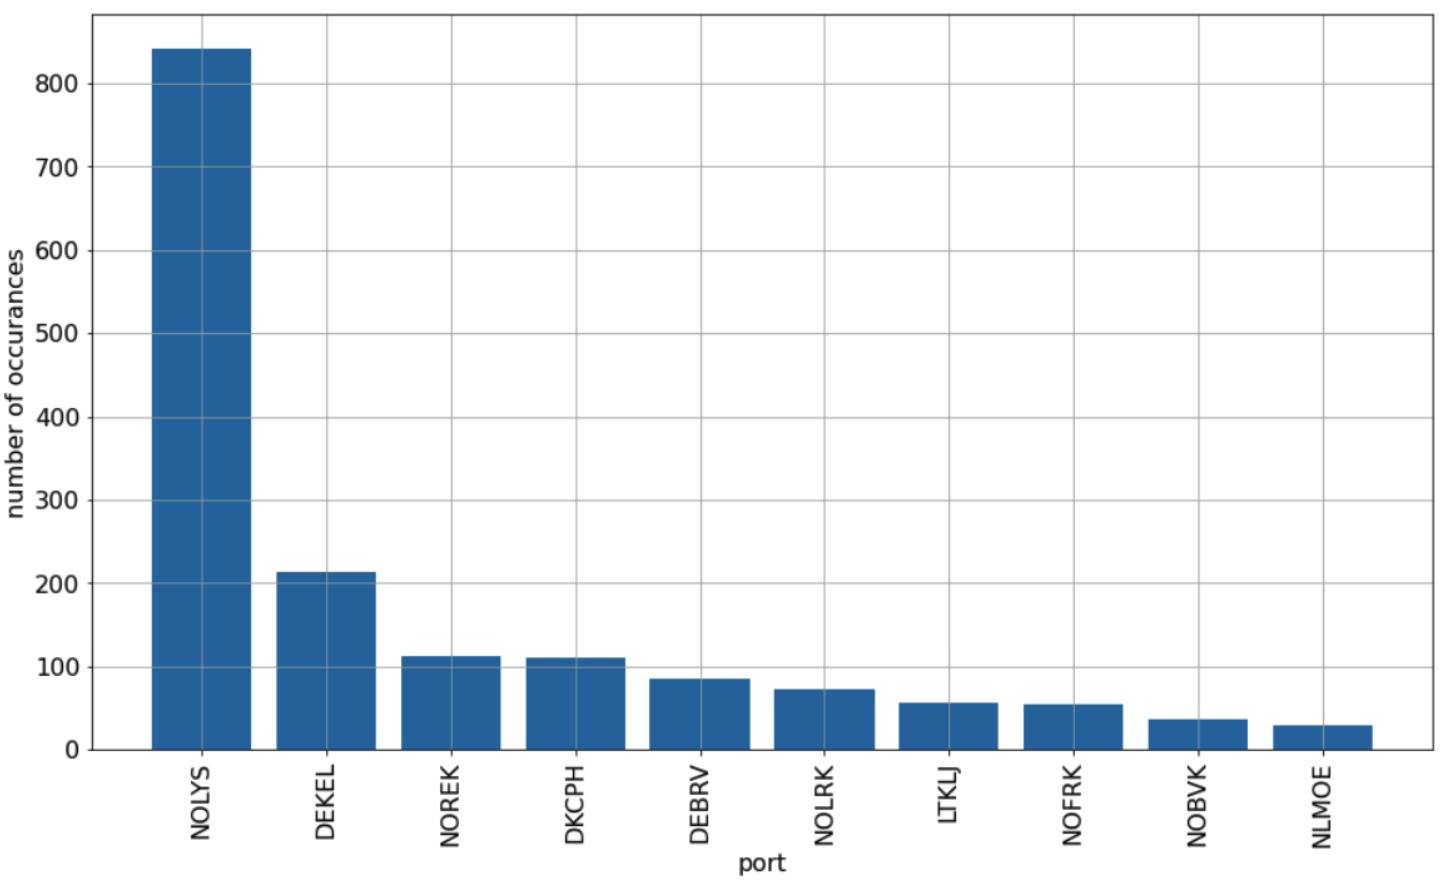
\includegraphics[width=.9\textwidth]{figures/apw/noosl_freq.png}
    \caption{Distribution of \textit{NextPort}s from \texttt{NOOSL}}
    \label{fig:apw_noosl_freq}
\end{figure}

When looking into the distributions of \textit{NextPort}s per segment it is even more apparent that the \textit{Other} segment (which includes passenger vessels) are responsible for the high number of voyages to \texttt{NOLYS}. \cref{fig:apw_noosl_segments} shows this as well as the \textit{Other} is the only segment that shares the same most frequent next port \texttt{NOLYS}. This means that a prediction algorithm using port frequencies would accurately predict the next destination ports for these other vessels, but not for the rest. Since the other vessels are responsible for 1568 out of 2009 transitions (78.05\%), considering vessel segmentation for predictions, and assuming every vessel always travel to its segment most frequent next port, a prediction algorithm could also become accurate for the remainder of the vessel segments which adds up to 21.95\% of all transition and probably most of the unique vessels. This is the basis used to estimate an improvement, or impact, factor for vessel segmentation on destination predictions.

\begin{figure}[htbp]
    \centering
    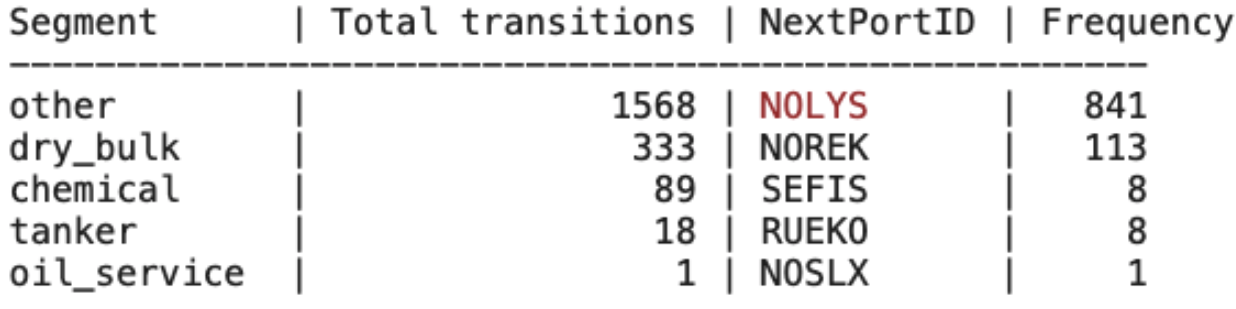
\includegraphics[width=.7\textwidth]{figures/apw/noosl_segments.png}
    \caption{Distribution of \textit{NextPort}s from \texttt{NOOSL} per segment}
    \label{fig:apw_noosl_segments}
\end{figure}

Furthermore, as \cref{fig:apw_noosl_dry_bulk} shows, when looking at the port frequency of the dry bulk cargo vessels, it is apparent that \texttt{NOLYS} is not even a contender for the most frequent next port. Therefore, a prediction method considering port frequencies would not be able to accurately predict the next destination port for any other vessel other than passenger vessels.

\begin{figure}[htbp]
    \centering
    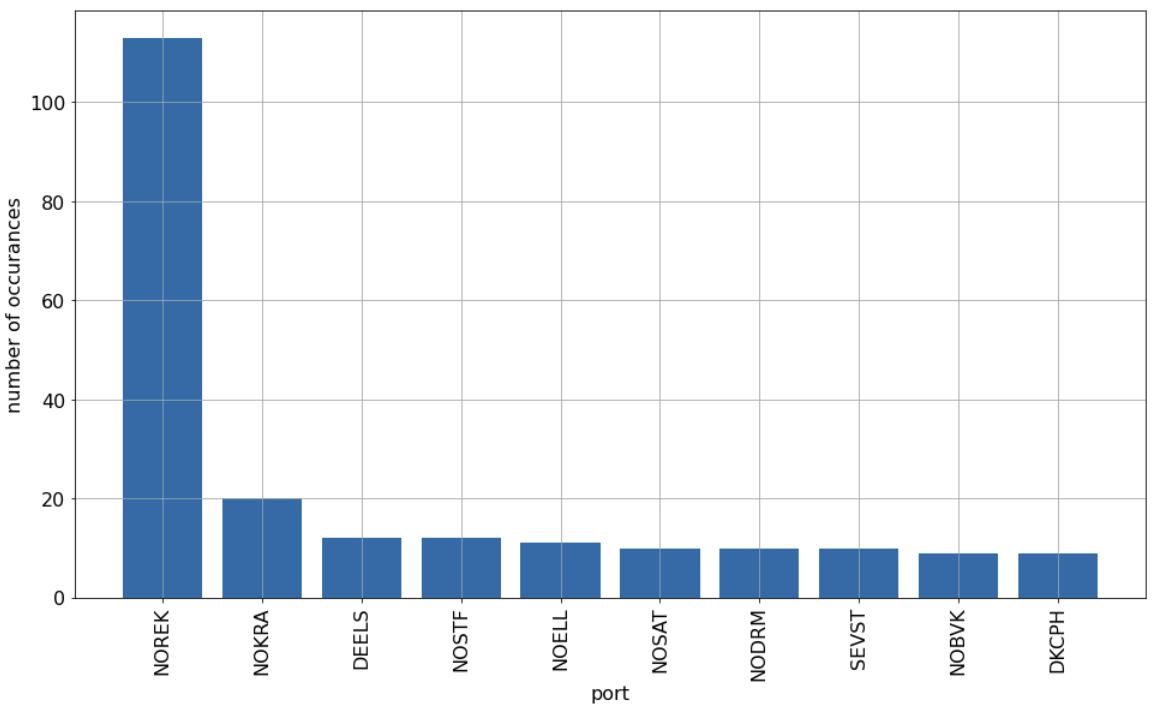
\includegraphics[width=.9\textwidth]{figures/apw/noosl_dry_bulk.png}
    \caption{Distribution of \textit{NextPort}s from \texttt{NOOSL} for the \textit{`dry bulk' segment}\label{fig:apw_noosl_dry_bulk}}
\end{figure}

Investigating sub-segments further confirms that a few numbers of vessels are responsible for most of all total transitions. \cref{fig:apw_noosl_subsegments} shows that the specific sub-segment \textit{`other - passenger'}, or passenger vessels, are responsible for 49.52\% of all transitions and nearly all voyages arrive at \texttt{NOLYS} after \texttt{NOOSL}. This means a prediction model could potentially be improved by 50\% if it would be aware of the sub-segment of each vessel for this particular port. \texttt{NOOSL} seems to be a port that shows the problem area quite well because it is a smaller port that receives a lower number of different vessels, and when there are multiple passenger vessels frequently arriving at it, they heavily skew the results in their favor.% chktex 8

\begin{figure}[htbp]
    \centering
    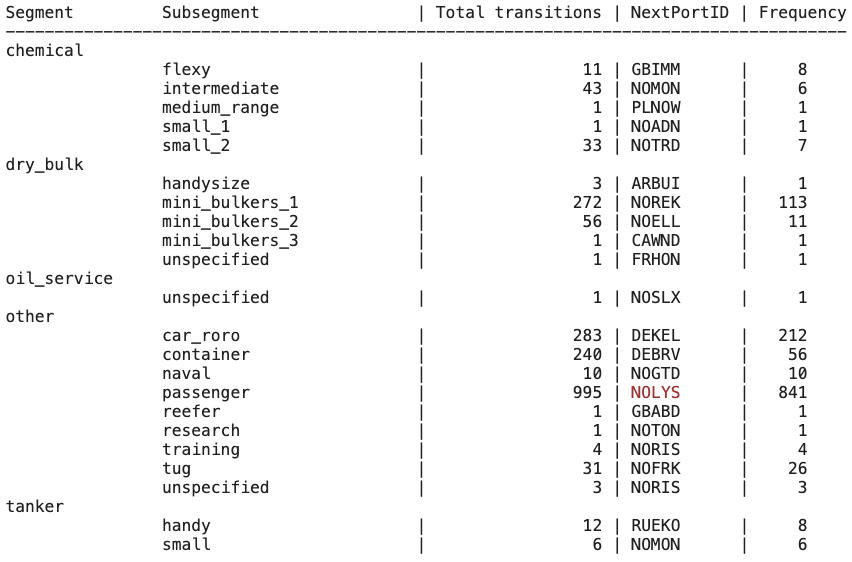
\includegraphics[width=.8\textwidth]{figures/apw/noosl_subsegments.png}
    \caption{Distribution of \textit{NextPort}s from \texttt{NOOSL} per sub-segment}
    \label{fig:apw_noosl_subsegments}
\end{figure}


\section{Trend analysis}
\label{sec:trend_analysis}

As already mentioned, for the trend analysis, a number of ports were selected based on their size and traffic. There were also a couple of known ports included in this dataset to easier interpret the results. The ports used in the analysis were:

\begin{itemize}
    \item \texttt{NLRTM} --- Rotterdam, Netherlands
    \item \texttt{NOOSL} --- Oslo, Norway
    \item \texttt{CNSHG} --- Shanghai, China
    \item \texttt{NLMSV} --- Maasvlakte, Netherlands
    \item \texttt{SGSIN} --- Singapore, Singapore
    \item \texttt{USHPY} --- Baytown, USA
    \item \texttt{BEANR} --- Antwerpen, Belgium
    \item \texttt{TWKHH} --- Kaohsiung, Taiwan
    \item \texttt{JPYOK} --- Yokohama, Japan
\end{itemize}

The same process as for the single-case analysis was conducted, but on a higher level as the main purpose of this study was to establish a trend in terms of a impact factor of vessel segmentation on port frequencies. \cref{fig:trend_freq} shows a similar version of the table used for the single port analysis (\cref{fig:apw_noosl_freq}) but also shows the number of transitions that differed from the most frequent next port when considering segments (i.e.\ the estimated improvement factor).

\begin{figure}[htbp]
    \centering
    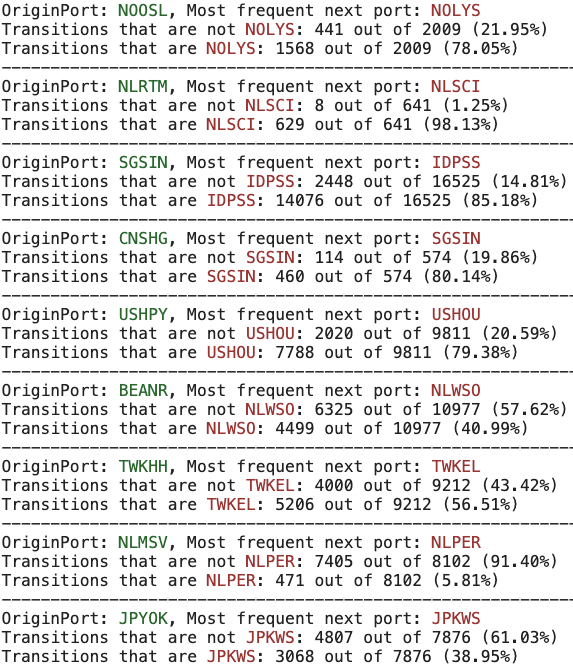
\includegraphics[width=.56\textwidth]{figures/apw/trend_frequency.png}
    \caption{Port frequencies and transition distribution as they relate to the most frequent next port for the selected ports}
    \label{fig:trend_freq}
\end{figure}

\begin{figure}[htbp]
    \centering
    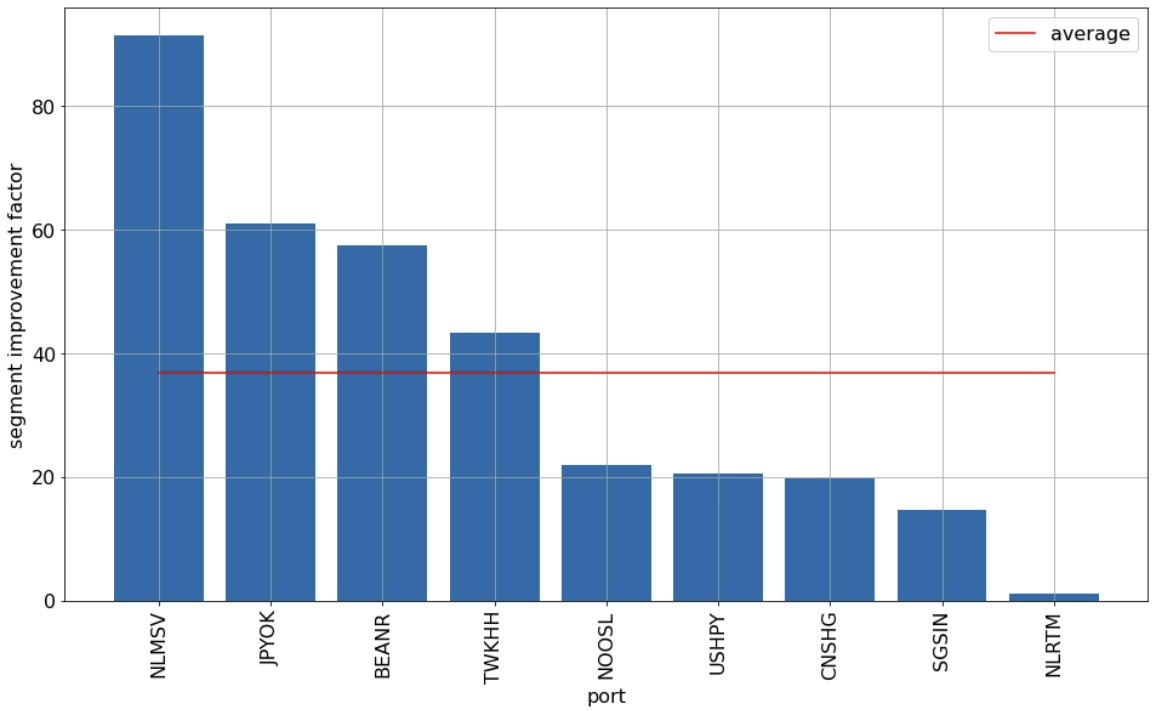
\includegraphics[width=.9\textwidth]{figures/apw/segment_improvement.png}
    \caption{Distribution of improvement factors for each origin port considering segments}
    \label{fig:segment_improvment}
\end{figure}

It is apparent that there are variances in improvement factors for different ports ranging from as low as \textit{1.25\%} to as high as \textit{91.40\%}. In the case of \texttt{NLRTM}, which is mostly a dry bulk port, there were no considerable improvements as almost all vessels are of the same segment. For the port \texttt{NLMSV}, the opposite was the case as there were a plethora of different types of vessels that frequented the port. \cref{fig:segment_improvment} shows the distribution of the improvement factor considering segments for each origin port as well as the overall average impact factor for these 9 ports which was \textit{36.88\%}.

Furthermore, when looking at the impact of sub-segments, as \cref{fig:subsegment_improvment} shows, it seems that the improvement factor has increased overall. For example, in the case of \texttt{NLRTM}, the improvement factor has increased from \textit{1.25\%} to \textit{19.66\%}, and although this varied for the different ports, the overall average improvement factor increased from \textit{36.88\%} to \textit{50.28\%}.

\begin{figure}[htbp]
    \centering
    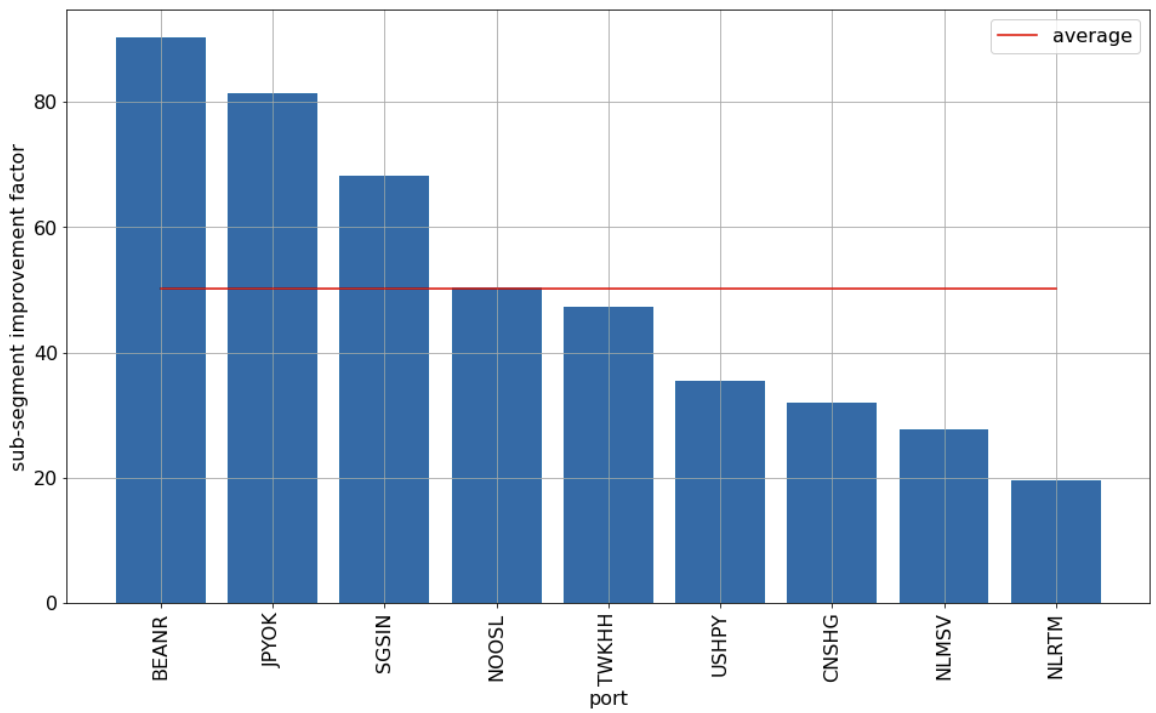
\includegraphics[width=.9\textwidth]{figures/apw/subsegment_improvement.png}
    \caption{Distribution of improvement factors for each origin port considering sub-segments}
    \label{fig:subsegment_improvment}
\end{figure}

A prediction method considering the frequencies of ports for vessel destination predictions would choose the most frequent next port for the predicted next destination. In this scenario, ignoring the vessel's type (segmentation) would give the wrong prediction for a lot of vessels from different segments in a lot of ports. The results from the feasibility study clearly indicates that applying the aspect of vessel segmentation to such models would definitively have an impact on prediction accuracy and, therefore, is worth investigating further.


\end{document}
